%\documentclass[PhD]{iitmdiss}
\documentclass[MS,twoside]{iitmdiss}
%\documentclass[MTech]{iitmdiss}
%\documentclass[BTech]{iitmdiss}
\usepackage{times}
 \usepackage{t1enc}

\usepackage{graphicx}
\usepackage{epstopdf}
\usepackage{hyperref} % hyperlinks for references.
\usepackage{amsmath} % easier math formulae, align, subequations \ldots


%%%%%%%%%%%%%%%%%%%%%%%%%%%%%%%
%\usepackage{ijcai17}


\usepackage{macros}

\usepackage{latexsym} 



\newcommand{\clearemptydoublepage}{\newpage{\cleardoublepage}}


\begin{document}

%%%%%%%%%%%%%%%%%%%%%%%%%%%%%%%%%%%%%%%%%%%%%%%%%%%%%%%%%%%%%%%%%%%%%%
% Title page

\title{Finite-time Analysis of Frequentist Strategies for Multi-armed Bandits}

\author{Subhojyoti Mukherjee}

\date{January 2018}
\department{COMPUTER SCIENCE AND ENGINEERING}

%\nocite{*}
\maketitle

%%%%%%%%%%%%%%%%%%%%%%%%%%%%%%%%%%%%%%%%%%%%%%%%%%%%%%%%%%%%%%%%%%%%%%
% Certificate

%\pagebreak
%\newpage
% \ 
%\thispagestyle{empty}
%\clearpage

\clearemptydoublepage
\certificate

\vspace*{0.5in}

\noindent This is to certify that the thesis titled {\bf Finite-time Analysis of Frequentist Strategies for Multi-armed Bandits}, submitted by {\bf Subhojyoti Mukherjee}, 
  to the Indian Institute of Technology, Madras, for
the award of the degree of {\bf Master of Science (Research)}, is a bona fide
record of the research work done by him under our supervision.  The
contents of this thesis, in full or in parts, have not been submitted
to any other Institute or University for the award of any degree or
diploma.

\vspace*{1.5in}

\begin{singlespacing}
\hspace*{-0.25in}
\parbox{2.5in}{
\noindent {\bf Dr. Balaraman Ravindran} \\
\noindent Research Guide \\ 
\noindent Professor \\
\noindent Dept. of Computer Science\\
\noindent IIT-Madras, 600 036 \\
} 
\hspace*{1.0in} 
\parbox{2.5in}{
\noindent {\bf Dr. Nandan Sudarsanam} \\
\noindent Research Co-Guide \\ 
\noindent Assistant Professor \\
\noindent Dept.  of  Management Studies\\
\noindent IIT-Madras, 600 036 \\
}  
\end{singlespacing}
\vspace*{0.25in}
\noindent Place: Chennai\\
Date: May 21, 2018


%%%%%%%%%%%%%%%%%%%%%%%%%%%%%%%%%%%%%%%%%%%%%%%%%%%%%%%%%%%%%%%%%%%%%%
% Acknowledgements
\clearemptydoublepage
\acknowledgements
%To be written.
I am grateful to my primary thesis advisor Dr. Balaraman Ravindran from Computer Science and Engineering Department at IIT Madras. Without his constant guidance, motivation and perseverance with me, none of these works would have been completed. His courses of Introduction to Machine Learning and Introduction to Reinforcement Learning were my first step into the research world. Not only these courses carried a wealth of information on the current state of literature in the respective fields but they used to be hugely competitive which used to constantly motivate me to strive for excellence. Apart from our formal meetings every week, I used to catch him in his office or in the corridors or anywhere in the department whenever I had any doubts and we used to converse on them. One of his greatest influences on me is to inculcate the constant urge to collaborate with as many interested people as possible, both inside and outside of my immediate field of research. This became a huge contributing factor in the research that I conducted for this thesis.

I am also grateful to my co-advisor Dr. Nandan Sudarsanam from Department of Management Studies at IIT Madras. It is from him that I first learned the most important factor of publication, how to properly write research papers in a concise and crisp manner. I fondly remember that how intensely he used to scrutinize my drafts for errors and incoherent ideas. His dedication and trust in my work are evident from this one incident during the ICML 2017 submission, when at 2 am in the night he called me up to correct portions of my draft. Also, his courses in Department of Management Studies are very enjoyable to attend and are very informative. Nobody can make you understand a complex idea in a simple way and yet retain all its subtleties as Nandan sir can and his courses used to reflect this idea.

Another person who had a profound influence on me is Dr. K.P. Naveen from Electrical Engineering Department at IIT Tirupati who advised me on a significant portion of this thesis. I first attended one of his courses on Introduction to Probability Theory here at IIT Madras (when he was INSPIRE Faculty member here) and instantly liked the way he taught the complex idea of Probability theory in simple terms. Even though the area of Multi-armed bandits is not his core research area, yet we collaborated on this topic which led to multiple publications. I fondly remember his rigor and patience with me while correcting the theoretical portions of my draft, the most important section of any bandit research paper.

I am also grateful to Dr. L.A. Prashanth from Computer Science and Engineering Department at IIT Madras in my initial days of research for advising me on a significant portion of stochastic multi-armed bandits. He is up-to-date with all the research work in this area and my interactions with him always led to new ideas and a broader way to look at a problem. All collaborations do not always lead to publications and I hope that our future interactions will lead to a more fruitful outcome.

While writing this thesis I must also acknowledge the contributions of Dr. Odalric-Ambrym Maillard from INRIA, SequeL Lab at Lille, France where I went for winter internship from September to December 2017. He is one of the most inspiring researchers that I met in my foray into the research world. He was always available at his office, always working on interesting ideas and always interested to listen to any idea that I came up with. The best thing about him that I can fondly relate to is that he never rejected any idea even though they were initially outrageous, but used to guide me slowly towards the reason on why they would fail in the long run. Similarly, I must also thank Dr. Branislav Kveton from Adobe Research, San Jose, whom I met on the sidelines of IJCAI 2017 who gave me a lot of feedback on how to improve my work on Thresholding Bandits. 

I am thankful to the other members of my committee for their constant support and guidance. I am especially thankful to Dr.  Sutanu Chakraborti for his trust on me. I fondly remember that whenever we used to meet we used to converse in Bengali and he used to constantly motivate me to work more. His course on Natural Language Processing is a very enjoyable course and the project on humor generation that I did under his supervision is one of most interesting projects I did in my IIT Madras coursework. I am also thankful to my Dr. Nirav P Bhatt and my committee chair Dr. P Sreenivasa Kumar for being always available for me.


I am thankful towards a host of my colleagues in the RISE Lab at Computer Science and Engineering Department where I spent a significant time while conducting research at IIT Madras. Thanks Patanjali for creating such an environment in the lab, conducive to research. I also thank my first roommate Priyesh for making my first semester so livable on the campus. In the course of time, I made more friends who contributed in making my life at IIT Madras memorable; Shashank, Siddharth, Deepak, Tarun, Madhuri, Ditty, Ahana, without you people life at IIT Madras would have been boring. There are several members of IPCV lab to whom I am grateful for making my stay at IIT Madras very memorable especially I must thank Nimisha, Abhijith, and Karthik for being such wonderful friends. I am also grateful towards my father, mother, brother, and sister-in-law Sarah for providing me constant motivation in my research and personal life. 

Last but not the least, I must thank Dr. A.P. Vijay Rengarajan from Electrical Engineering Department at IIT Madras. He was also conducting research for his doctoral studies in the IPCV lab and it his from him that I learned the true meaning of dedication towards research. This dedication of him, of course, showed up in all the publications he got but most of all he was always there, listening to all my concerns on a host of issues that I faced in my research and personal life. Vijay without you life at IIT Madras would not have been same.

Finally, I must acknowledge the influence of Dr. Sven Koenig whom I met on the sidelines of IJCAI 2017 in the "Lunch with  A Fellow" event. That four-hour interaction with him is a memory I cherish because we talked about every possible aspect of a researcher's life and how to conduct good research. In the end, he said to me the three mantras of conducting good research; shed ego, collaborate and learn something new every day.

%Every day from 9 am to 6 pm for 365 days a year he was available in the lab, sitting in front of his desktop and working tirelessly.


%%%%%%%%%%%%%%%%%%%%%%%%%%%%%%%%%%%%%%%%%%%%%%%%%%%%%%%%%%%%%%%%%%%%%%
% Abstract
\clearemptydoublepage
\abstract

%\noindent KEYWORDS: \hspace*{0.5em} \parbox[t]{4.4in}{Reinforcement Learning, Bandits, UCB, EUCBV, Thresholding Bandits,  AugUCB, changepoint detection, SECPD.}

\noindent KEYWORDS: \hspace*{0.5em} \parbox[t]{4.4in}{Reinforcement Learning, Stochastic Bandits, UCB, UCBV, EUCBV, Thresholding Bandits, APT, AugUCB}

\vspace*{24pt}
\noindent The thesis studies the following topics in the area of Reinforcement Learning: Multi-armed Bandits, Multi-armed bandits in stationary distribution with the goal of cumulative regret minimization and Thresholding bandits in pure exploration setting. The common underlying theme is the study of bandit theory and its application in various types of environments. In the first part of the thesis, we study the classic multi-armed bandit problem in stationary distribution, one of the first setting studied by the bandit community and which successively gave rise to several new directions in bandit theory. We propose a novel algorithm in this setting and compare both theoretically and empirically its performance against the available algorithms in this setting. Our proposed algorithm called Efficient-UCB-Variance (EUCBV) is the first arm-elimination algorithm which uses variance estimation to eliminate arms as well as achieve an order optimal regret bound. Empirically, we show that EUCBV outperforms most of the state-of-the-art algorithms in the considered environments. In the next part, we study a very specific type of stochastic multi-armed bandit setup called the thresholding bandit problem and discuss extensively on its usage, available state-of-the-art algorithms on this setting and our solution to this problem. We propose the Augmented-UCB algorithm which again uses variance and mean estimation along with arm elimination technique to conduct exploration. We give theoretical guarantees on the expected loss of our algorithm and also analyze its performance against state-of-the-art algorithms in numerical simulations in multiple synthetic environments. 

%The thesis studies the following topics in the area of Reinforcement Learning: Multi-armed Bandits, Multi-armed bandits in stationary distribution with the goal of cumulative regret minimization and Thresholding bandits in pure exploration setting. The common underlying theme is the study of bandit theory and its application in various types of environments. We start with a general introduction to Multi-armed bandits, its connection to the wider reinforcement learning theory and then we discuss the various types of bandits available in the literature. Then we delve deep into the classic multi-armed bandit problem in stationary distribution, one of the first setting studied by the bandit community and which successively gave rise to several new directions in bandit theory. We propose a novel algorithm in this setting and compare both theoretically and empirically its performance against the available algorithms in this setting. Subsequently, we study a very specific type of bandit setup called the thresholding bandit problem and discuss extensively on its usage, available state-of-the-art algorithms on this setting and our solution to this problem. We give theoretical guarantees on the expected loss of our algorithm and also analyze its performance against state-of-the-art algorithms in numerical simulations in multiple synthetic environments. 

%, and analysis of bandit theory in piece-wise stationary distributions

%Finally, we study the notion of piece-wise stationary distribution and how available bandit algorithms can be modified to perform well in this setting. We propose a set of algorithms for this setting with the goal of minimizing cumulative regret which uses various techniques ranging from changepoint detection mechanism to aggregation of experts.

%\pagebreak

%%%%%%%%%%%%%%%%%%%%%%%%%%%%%%%%%%%%%%%%%%%%%%%%%%%%%%%%%%%%%%%%%
% Table of contents etc.
\clearemptydoublepage
\begin{singlespace}
\tableofcontents
%\thispagestyle{empty}

\clearemptydoublepage
\listoftables
\addcontentsline{toc}{chapter}{LIST OF TABLES}


\clearemptydoublepage
\listoffigures
\addcontentsline{toc}{chapter}{LIST OF FIGURES}
\end{singlespace}


%%%%%%%%%%%%%%%%%%%%%%%%%%%%%%%%%%%%%%%%%%%%%%%%%%%%%%%%%%%%%%%%%%%%%%
% Abbreviations
\clearemptydoublepage
\abbreviations

\noindent 
\begin{tabbing}
xxxxxxxxxxx \= xxxxxxxxxxxxxxxxxxxxxxxxxxxxxxxxxxxxxxxxxxxxxxxx \kill
%\textbf{RL}   \> Reinforcement Learning \\
%\textbf{MAB} \> Multi-armed Bandit \\
%\textbf{SMAB} \> Stochastic Multi-armed Bandit \\
%\textbf{UCB} \> Upper Confidence Bound \\
%\textbf{MOSS} \> Minimax Optimal Strategy in the Stochastic case \\
%\textbf{UCBV} \> Upper Confidence Bound Variance \\
%\textbf{OCUCB} \> Optimally Confident Upper Confidence Bound \\
%\textbf{KLUCB} \> Kullback–Leibler Upper Confidence Bound \\
%\textbf{TS} \> Thompson Sampling \\
%\textbf{EUCBV} \> Efficient Upper Confidence Bound Variance \\
%\textbf{TBP} \> Thresholding Bandit Problem \\
%\textbf{UCBE} \> Upper Confidence Bound Exploration\\
%\textbf{UCBEV} \> Upper Confidence Bound Exploration Variance\\
%\textbf{UA} \> Uniform Allocation \\
%\textbf{SR} \> Successive Reject \\
%\textbf{CSAR} \> Combinatorial Successive Accept Reject \\
%\textbf{APT} \> Anytime Parameter-free Thresholding \\
%\textbf{AugUCB} \> Augmented Upper Confidence Bound \\
\textbf{APT} \> Anytime Parameter-free Thresholding \\
\textbf{AugUCB} \> Augmented Upper Confidence Bound \\
%BIB
\textbf{BU} \> Bayes-UCB \\
\textbf{CCB} \> Combined Confidence Bound \\
%CPD
%CPDI
\textbf{CSAR} \> Combinatorial Successive Accept Reject \\
%CUSUM
%DBLP
\textbf{DMED} \> Deterministic Minimum Empirical Divergence \\
\textbf{DTS} \> Discounted Thompson Sampling \\
\textbf{DUCB} \> Discounted UCB \\
%DVI
\textbf{EUCBV} \> Efficient Upper Confidence Bound Variance \\
%EVE
\textbf{EXP3} \> Exponential Exploration Exploitation \\
\textbf{EXP3IX} \> EXP3 Implicit Exploration \\
\textbf{GCTS} \> Global Change-ponit Thompson Sampling \\
%GK
%IITM
\textbf{KL} \> Kullback–Leibler \\
\textbf{KLUCB} \> Kullback–Leibler Upper Confidence Bound \\
%KT
%LHS
\textbf{LUCB} \> Lower Upper Confidence Bound \\
\textbf{MAB} \> Multi-armed Bandit \\
\textbf{MDP} \> Markov Decision Process \\
\textbf{MOSS} \> Minimax Optimal Strategy in the Stochastic case \\
%MS
\textbf{OCUCB} \> Optimally Confident Upper Confidence Bound \\
%\textbf{OTS} \> Oracle Thompson Sampling \\
%PDF
\textbf{RL}   \> Reinforcement Learning \\
\textbf{RExp3}   \> Restarting EXP3 \\
\textbf{SAR} \> Successive Accept Reject \\
%SECPD
\textbf{SMAB} \> Stochastic Multi-armed Bandit \\
\textbf{SR} \> Successive Reject \\
\textbf{SW-UCB} \> Switching Window UCB \\ 
\textbf{TBP} \> Thresholding Bandit Problem \\
\textbf{TS} \> Thompson Sampling \\
\textbf{UA} \> Uniform Allocation \\
\textbf{UCB} \> Upper Confidence Bound \\
\textbf{UCBE} \> Upper Confidence Bound Exploration\\
\textbf{UCBEV} \> Upper Confidence Bound Exploration Variance\\
\textbf{UCBV} \> Upper Confidence Bound Variance \\
%URL



\end{tabbing}

%\pagebreak

%%%%%%%%%%%%%%%%%%%%%%%%%%%%%%%%%%%%%%%%%%%%%%%%%%%%%%%%%%%%%%%%%%%%%%
% Notation

\clearemptydoublepage
\chapter*{\centerline{NOTATION}}
\addcontentsline{toc}{chapter}{NOTATION}

\begin{singlespace}
\begin{tabbing}
xxxxxxxxxxx \= xxxxxxxxxxxxxxxxxxxxxxxxxxxxxxxxxxxxxxxxxxxxxxxx \kill
\textbf{$T$} \> Time horizon\\
\textbf{$\A$} \> Set of arms\\
\textbf{$K$} \> Total number of arms\\
\textbf{$\pi$}   \> Policy of an agent \\
\textbf{$D_i$}  \> Reward distribution of $i$-th arm \\
\textbf{$r_i$}  \> Expected mean of $D_i$ for the $i$-th arm \\
\textbf{$\hat{r}_i$}  \> Sample mean of the $i$-th arm \\
\textbf{$X_{i,t}$} \> Reward obtained for the $i$-th arm at the $t$-th timestep\\
\textbf{$z_i$}  \> Number of times arm $i$ is pulled\\
\textbf{$\sigma_i$} \> Standard Deviation of the $i$-th arm\\
\textbf{$v_i$} \> Variance of the $i$-th arm\\
\textbf{$\Delta_i$} \> Gap of the $i$-th arm\\
\textbf{$\Delta$} \> Minimal gap amongst all arms\\
\textbf{$\tau$} \> Threshold\\
\textbf{$H_1$} \> Hardness with Mean-$1$\\
\textbf{$H_2$} \> Hardness with Mean-$2$\\
\textbf{$H_{\sigma,1}$} \> Hardness with Mean and Standard Deviation-$1$\\
\textbf{$H_{\sigma,2}$} \> Hardness with Mean and Standard Deviation-$2$\\
\textbf{$\rho$} \> Parameter for tuning length of of confidence interval\\
\textbf{$\psi$} \> Exploration parameter\\
\textbf{$m$} \> Round number\\
\textbf{$R_T$} \> Cumulative regret till horizon $T$\\
\textbf{$SR_t$} \> Simple regret at $t$-th timestep\\
\end{tabbing}
\end{singlespace}

%\pagebreak
%\clearpage

% The main text will follow from this point so set the page numbering
% to arabic from here on.



%%%%%%%%%%%%%%%%%%%%%%%%%%%%%%%%%%%%%%%%%%%%%%%%%%
% Introduction.
\clearemptydoublepage
\pagenumbering{arabic}
\chapter{Introduction to Bandits}
\label{chap:intro}

\section{Reinforcement Learning}
\label{intro}
In today's world artificial intelligence has proved to be a game-changer in designing agents that interact with an evolving environment and make decisions on the fly. The main goal of artificial intelligence is to design artificial agents that make dynamic decisions in an evolving environment. In pursuit of these the agent can be thought of as making a series of  sequential decisions by interacting with the dynamic environment which provides it with some sort of feedback after every decision which the agent incorporates into its decision-making strategy to formulate the next decision to be made. A large number of problems in science and engineering, robotics and game playing, resource management, financial portfolio management, medical treatment design, ad placement, website optimization and packet routing can be modeled as sequential decision-making under uncertainty. Many of these real-world interesting
sequential decision-making problems can be formulated as reinforcement learning (RL) problems (\citep{bertsekas1996neuro}, \citep{sutton1998reinforcement}). In an RL problem, an agent interacts with a dynamic, stochastic, and unknown environment, with the goal of finding an action-selection strategy or policy that optimizes some long-term performance measure. Every time when the agent interacts with the environment it receives a signal/reward from the environment based on which it modifies its policy. The agent learns to optimize the choice of actions over several time steps which is learned from the sequences of data that it receives from the environment. This is the crux of online sequential learning. An illustrative image depicting the reinforcement learning scenario is shown in Figure \ref{fig:rl}.

	This is in contrast to supervised learning methods that deal with labeled data which are independently and identically distributed (i.i.d.) samples from the domain and train some classifier on the entire training dataset to learn the pattern of this distribution to predict future samples (test dataset) with the assumption that it is sampled from the same domain, whereas the RL agent learns from the samples that are collected from the trajectories generated by its sequential interaction with the system. For an RL agent the trajectory consists of a series of sequential interactions whereby it transitions from one state to another following some dynamics intrinsic to the environment while collecting the reward till some stopping condition is reached. This is known as an episode. For a single-step interaction, i.e., when the episode terminates after a single transition, the problem is captured by the multi-armed bandit (MAB) model. Our work will focus on this idea of MAB model.

\begin{figure}[!th]
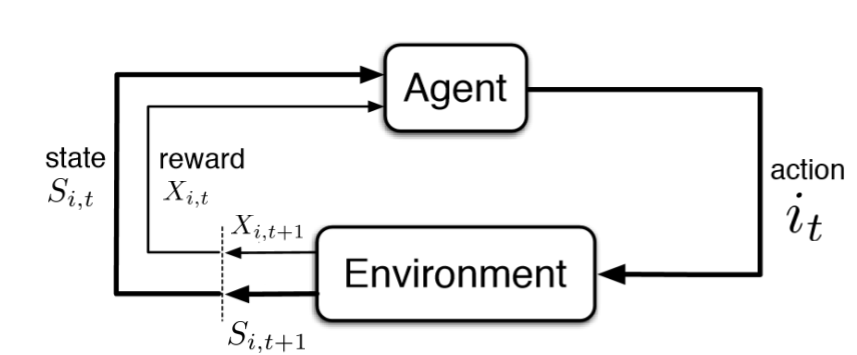
\includegraphics[scale=0.5]{Chapter1/img/RL1.png}
\caption{Reinforcement Learning}
\label{fig:rl}
\end{figure}

%To express an RL problem more formally, we have to define the idea of Markov Decision Process (MDP) which consists of states, actions, transition probabilities and rewards which in turn helps in deciding the strategy to be followed by the agent. 

%An MDP consists of states


\section{Connection between Reinforcement Learning and Bandits}
\label{conn:Bandits}
As defined in the previous section, an episode consists of a series of sequential interaction whereas agent transitions from one state to another based on some intrinsic dynamics of the environment while collecting the rewards and choosing actions based on some action-selecting strategy. Now, for a single-step interaction, i.e., when the episode terminates after a single transition, the problem is captured by the multi-armed bandit (MAB) model. In fact, the MAB model can be considered as a single looping state when the agent after taking an action and observing the reward transitions back to the same state. That single looping state consists of several finite number of actions which are called as arms.

    The name bandit originated from the concept of casino slot machine where there are levers which are called as arms and the learner can pull one lever and observes the reward associated with that arm which is sampled from a distribution associated with the specific arm. This game is repeated $T$ times and the goal of the learner is to maximize its profit. 


\section{Why study Bandits?}
\label{study}
There are multiple reasons to study the interesting area of bandits. First of all, bandits are the cornerstone of understanding the general reinforcement learning area. Infact, bandits helps us to understand the idea of \textit{exploration-exploitation} dilemma which is the basis to build full, multi-state, general reinforcement learning ideas. Secondly, as stated in \citet{maillard2011apprentissage}, even $50$ years after \cite{robbins1952some} introduced the first idea of bandits, there are many interesting and fruitful areas where bandit concept can be extended in both practical and theoretical terms. Finally, there are several real-life industrial applications ranging from recommendation systems, game theory to anomaly detection where bandit applications have been found to perform exceptionally well. All of these forces us to delve deep into a systemic research of bandits.

\section{Motivation}
\label{motivation}
The MAB model fits very well in various real-world scenarios that can be modeled as decision-making under uncertainty  problems. Some of which are as follows:-
\begin{enumerate}
\item \emph{Online Shop Domain:} In the online shop domain \citep{ghavamzadeh2015bayesian}, a retailer aims to maximize profit by sequentially suggesting products to online shopping customers. In this scenario, at every timestep, the retailer displays an item to a customer from a pool of items which has the highest probability of being selected by the customer. The one-step interaction ends when the customer selects or does not select a product (which will be considered as a loss to the retailer). This feedback is incorporated by the learner as a feedback from the environment and it modifies its policy for the next suggestion. This process is repeated till a pre-specified number of times with the retailer gathering valuable information regarding the customer from this behaviour and modifying its policy to display other items to different customers. In its simplest form,  this can be modeled as a stochastic MAB problem which is studied in the first part of the thesis.
\item \emph{Medical Treatment Design:} Another interesting domain that MAB model was first studied was for the medical treatment design \citep{thompson1933likelihood},\citep{thompson1935theory}. Here at every timestep, the learner chooses to administer one out of several treatments sequentially on a stream of patients who are suffering from the same ailment (say). Let's also assume that there is a single treatment which will be able to alleviate the patients from their disease. Here, the one-step interaction ends when the patient responds well or does not respond well to the treatment whereby the learner modifies its policy for the suggestion to the next patient. The goal of the learner is to quickly converge on the best treatment so that whenever a new patient comes with the same ailment, the learner can suggest the best treatment which can relieve the patient of its ailment with a high probability. This problem can also be modeled as a stochastic MAB problem.
\item \emph{Financial Portfolio Management:} In financial portfolio management MAB models can also be used. Here, the learner is faced with the choice of selecting the most profitable stock option out of several stock options. The simplest strategy where we can employ a bandit model is this; at the start of every trading session, the learner suggests a stock to purchase worth Re $1$, while at the closing of the trading session it sells off the stock to witness its value after a day's trading. The profit recorded is treated as the reward revealed by the environment and the learner modifies its policy for the next day. Let's assume that no new stock options are being introduced over the considered time horizon and there is a single best stock option which if selected in perpetuity will always give the best returns. Then, the goal of the learner is reduced to identifying the best stock option as quickly as possible. This is another interesting variation which can be modeled as a stochastic MAB problem.
\item \emph{Product Selection:} A company wants to introduce a new product in the market and there is a clear separation of the test phase from the commercialization phase. In this case, the company tries to minimize the loss it might incur in the commercialization phase by testing as much as possible in the test phase. So from the several variants of the product that is in the test phase, the learning learner must suggest the product variant(s) whose qualities are above a particular threshold $\tau$ at the end of the test phase that has the highest probability of minimizing the loss in the commercialization phase. A similar problem has been discussed for single best product variant identification without threshold in \citet{bubeck2011pure}. This problem can be modeled as a stochastic thresholding MAB problem which is studied in the second part of the thesis.
\item \emph{Mobile Phone Channel Allocation:} Another similar problem as above concerns channel allocation for mobile phone communications \citep{audibert2009exploration}. Here there is a clear separation between the allocation phase and communication phase whereby in the allocation phase a learner has to explore as many channels as possible to suggest the best possible set of channel(s) whose qualities are above a particular threshold $\tau$. The threshold may depend on the subscription level of the customer such that with the higher subscription the customer is allowed better channel(s) with the $\tau$ set high. Each evaluation of a channel is noisy and the learning algorithm must come up with the best possible set of suggestions within a very small number of attempts. This setting can also be modeled as a stochastic thresholding MAB problem.
\item \emph{Anomaly Detection and Classification:} MABs can also be used for anomaly detection where the goal is to seek out extreme values in the data. Anomalies may not always be naturally concentrated which was shown in  \citet{steinwart2005classification}. To implement a MAB model the best possible way is to define a cut-off level $\tau$ and classify the samples above this level $\tau$ as anomalous along with a tolerance factor which gives it a degree of flexibility. Such an approach has already been mentioned in \citet{streeter2006selecting} and further studied in \citet{locatelli2016optimal}. Finally, this is also an interesting variation which can be modeled as a stochastic thresholding MAB problem.
\end{enumerate}


%    In all the above examples the MAB model performs well mainly because all of them suffer from \textit{exploration-exploitation dilemma}. This is characterized by action-selection choice faced by the learner where it must decide whether to stay with the action yielding highest reward till now or to explore newer actions which might be more profitable in the long run. MAB's are suited for such scenarios because 
%\begin{enumerate}
%\item They are easy to implement.
%\item The switch between exploration and exploitation is more well defined theoretically.
%\item They perform well empirically.
%\end{enumerate}



\section{Types of Information Feedback}
\label{feed}
In an online sequential setting, the feedback that the learner receives from the environment can be characterized into three broad categories, full information feedback, partial information feedback and bandit feedback. 


	To illustrate the different types of feedback we will take help of the following example. Let a learner be given a set of actions $i\in\A$ such that $|A|=K$. Let, the environment be such that each action has a probability distribution $D_i$ attached to it which is fixed throughout the time horizon $T$. The learning proceeds as follows:-

\begin{algorithm}[!th]
\caption{An online sequential game}
\label{alg:OSeqGame}
\begin{algorithmic}
\State {\bf Input:} Time horizon $T$, $K$ number of arms with unknown parameters of reward distribution
\State \For{ each timestep $t=1,2,\ldots, T$}
\State The environment chooses a reward $r_{i,t},\forall i\in\A$.
\State The learner chooses $m$ actions such that $m < K$, where $A$ is the set of arms and $|A|=K$.
\State The learner observes the reward $R_{m,t}=F\left( r_{i,t}\right)$.
\State \EndFor
\end{algorithmic}
\end{algorithm}

%Let $G(V,E)$ denote a graph where $V$ denotes the set of nodes in the graph and $E$ denotes the set of edges of the graph. Let there be a single starting node, denoted by $\mathcal{s}\in V$ from where the learner must start and try to reach the destination node denoted by $\mathcal{d}\in V$. Each edge has a delay associated with it which is unknown to the learner. This delay is an $i.i.d$ random variable from the distribution $D_{ij}$ associated with the edge $e_{ij}$ between the vertices $v_i$ and $v_j$. Whenever an edge is chosen the environment reveals to the learner  At every timestep the learner chooses a set of edges and receives some form of feedback from the environment. The goal of the learner is to find the path from $s$ to $d$ which has the minimum delay associated with it. 


\subsection{Full information feedback}
In full information feedback, when a learner selects $m$ actions then the environment reveals the rewards of all the actions $i\in \A$. Hence, in this form of feedback  the learner observes $R_{m,t} = \lbrace r_{i,t},\forall i\in\A\rbrace$.


\subsection{Partial information feedback}
In partial information feedback, when a learner selects $m$ actions then the environment reveals the rewards of only those $m$ actions for $m\in \A$. Hence, in this form of feedback  the learner observes $R_{m,t} = \lbrace r_{m,t},\forall m\in\A\rbrace$. This is also sometimes called the semi-bandit feedback.


\subsection{Bandit feedback}
In bandit feedback, when a learner selects $m$ actions then the environment reveals a cumulative reward of those $m$ actions for $m\in \A$. Hence, in this form of feedback  the learner observes $R_{m,t} = \sum_{q=1}^{m} r_{q,t}$. Note, that when $m=1$, then the learner observes the reward of only that action that it has chosen out of $K$ actions.





\section{Different types of Bandits}
\label{types}
In this section, we discuss the various types of bandits that are available in the literature. 


\subsection{Types of Bandits based on Environment}


\subsubsection{Stochastic Bandits}
In stochastic bandits, the distribution associated with each of the arms remains fixed throughout the time horizon $T$. Some of the notable papers associated with this type of setup are \citet{robbins1952some}, \citet{lai1985asymptotically},  \citet{agrawal1995sample}, \citet{auer2002finite}, \citet{auer2010ucb}, \citet{audibert2009minimax}, \citet{lattimore2015optimally}, etc. Chapter \ref{chap:SMAB} and Chapter \ref{chap:EUCBV} is based on this setup where we discuss extensively on the latest state-of-the-art algorithms.



\subsubsection{Non-stochastic Bandits}

In non-stochastic setting, the distribution associated with each arm varies over the duration of the play. Two notable examples of this are:-

\begin{enumerate}
\item \textbf{Adversarial bandits: } One of the first settings that has greatly motivated the studies in bandit literature is the \textit{adversarial setting}. In this setting, at every timestep, an adversary chooses the reward for each arm and then the learner selects an arm without the knowledge of the adversary's choice. The adversary may or may not be oblivious to the learner's strategy and this forces the learner to employ a randomized algorithm to confuse the adversary. Previous works on this have focused on constructing different types of exponential weighting algorithms that are based on the Hedge algorithm that has been proposed before in \citet{littlestone1994weighted},\citet{freund1995desicion} and analyzed in \citet{auer1995gambling}. Further variants of this strategy called EXP3 \citep{auer2002nonstochastic}, \citep{auer2002using} and EXP3IX \citep{kocak2014efficient} have also been proposed which incorporates different strategies for exploration to minimize the loss of the learner.


%In adversarial bandits, an adversary decides the payoff for each arm before the learner selects an arm. This adversary may or may not be oblivious to the learning algorithm employed by the learner. In each of these cases, a different guarantee on the performance of the learner can be arrived at. Some of the important works in this setting can be found in \citet{auer2002nonstochastic}, \citet{auer2002using}, \citet{kocak2014efficient}.

\item \textbf{Piece-wise stationary:} Striding between the two contrasting settings of SMAB and adversarial bandits is the piece-wise stochastic multi-armed bandit setting where there are a finite number of changepoints when the distribution associated with each arm changes abruptly. Hence, this setting is neither as pessimistic as adversarial setting nor as optimistic as the stochastic setting. Therefore, the two broad class of algorithms mentioned before fail to perform optimally in this setting. Several interesting solutions have been proposed before for this setting which can be broadly divided into two categories, passively adaptive and actively adaptive strategies. Passively adaptive strategies like Discounted UCB (DUCB) \citep{kocsis2006discounted}, Switching Window UCB (SW-UCB)  \citep{garivier2011upper} and Discounted Thompson Sampling (DTS) \citep{raj2017taming} do not actively try to locate the changepoints but rather try to minimize their losses by concentrating on past few observations. Similarly, algorithms like Restarting Exp3 (RExp3) \citep{DBLP:journals/corr/BesbesGZ14} behave pessimistically as like Exp3 but restart after pre-determined phases. Hence, RExp3 can also be termed as a passively adaptive algorithm. On the other hand, actively adaptive strategies like Adapt-EVE \citep{hartland2007change}, Windowed-Mean Shift \citep{yu2009piecewise}, EXP3.R \citep{allesiardo2017non}, CUSUM-UCB \citep{liu2017change} try to locate the changepoints and restart the chosen bandit algorithms. Also, there are Bayesian strategies like Global Change-Point Thompson Sampling (GCTS)\citep{mellor2013thompson} which uses Bayesian changepoint detection to locate the changepoints. 


%Another setup under this setting can be the piece-wise stationary setting. In this setting, the distribution associated with each arm is not fixed throughout the time horizon and changes either arbitrarily at particular changepoints, or changes at a fixed period. The distribution associated with each arm then remains fixed till the next changepoint is encountered. Several recent works have focussed on this such as  \citep{garivier2011upper}, \citep{mellor2013thompson}, and \citep{allesiardo2017non}. In our thesis, chapter \ref{chap:psbandit} is based on this setting. 
\end{enumerate}




%\subsubsection{Contextual Bandits}
%
%The idea of clustering has been extensively studied in the contextual bandit setup, an extension of the MAB where side information or features are attached to each arm. The clustering is done over the features representing the arms to capture the complexity of the problem better when a large number of arms are involved. Typical examples of this setting are in a web-advertising domain, news article selection, etc. Some notable papers available for this setting are   \citet{auer2002using}, \citet{langford2008epoch}, \citet{li2010contextual}, \citet{beygelzimer2011contextual}, \citet{slivkins2014contextual},etc. 


%

%Clustering has been extensively studied in the area of contextual MAB. In contextual MAB, there are side-information or features attached to each arm (see  \citet{auer2002using,langford2008epoch,li2010contextual,beygelzimer2011contextual, slivkins2014contextual}).   \cite{bui2012clustered,cesa2013gang,gentile2014online}. Please note that we do not cluster over the context rather we cluster the arms into groups.




\subsection{Types of Bandits based on goal}

In bandit literature, based on the goal we can divide bandits into several categories. To illustrate this we put forward a simple scenario let us consider a stochastic bandit scenario where there are $K$ arms labeled $i=1,2,\ldots, K$ with their expected means of reward distributions ($D_i$) be denoted by $r_i$. Also let there be single optimal arm $*$ such that $r^* = \max_{i\in\A}r_i$. 



\subsubsection{Cumulative regret minimization}
In cumulative regret minimization the goal of the bandit is to minimize the cumulative regret which is the total loss suffered by the learner throughout the time horizon $T$ for not choosing the optimal arm. Formally, we can define the cumulative regret as,

\begin{eqnarray}
R_{T} = \sum_{t=1}^{T}r^* - \sum_{i\neq *}r_{i}n_{i,T} \label{eqn:chap1:regret}
\end{eqnarray}

where, $n_{i,T}$ is the number of times the learner has chosen arm $i$ over the entire horizon $T$. We can further reduce equation \ref{eqn:chap1:regret} to obtain,

\begin{align*}
R_{T} = \sum_{t=1}^{T}r^* - \sum_{i\neq *}r_{i}n_{i,T} = \sum_{i=1}^{K}\Delta_{i}n_{i,T}
\end{align*}

where $\Delta_{i}=r^* - r_i$ is called the gap between the optimal and the sub-optimal arm.

\subsubsection{Simple regret minimization}
In simple regret minimization the goal of the bandit is to minimize the instantaneous regret that is suffered at any  timestep by the learner. Formally, the simple regret at $t$-th timestep where $J_n\in\A$ is the recommendation by the learner at timestep $t$ is defined,

\begin{align*}
SR_{t} = r^* - r_{J_{n}} = \Delta_{J_n}
\end{align*}

where $\Delta_{J_n}$ is the instantaneous gap between the expected mean of the optimal arm and the recommended arm by the learner. In the pure exploration setting the learner tries to minimize the simple regret and we study a very similar setting in chapter \ref{chap:tbandit1} and chapter \ref{chap:tbandit2}. 

\subsubsection{Weak Regret minimization}
In the non-stochastic scenario, when the distribution associated with each arm changes, the notion of regret is defined differently than cumulative regret. In this scenario, considering that there is a single best arm, the learner is more interested in minimizing the worst-case regret. Formally, for any sequence of actions $\left( j_1, \ldots , j_T \right)$ chosen by the learner over the time horizon $T$, the weak regret for single best action is defined as the difference between,
\begin{align*}
G_{\max}(j_1,\ldots,j_T) - G_{\pi}(T)
\end{align*}
where, $G_{\max}(j_1,\ldots,j_T) = \max_{i\in\A}\sum_{t=1}^{T}X_{i_t}$ is the return of the globally best action over the entire horizon $T$, $X_{i_t}$ is the reward observed for the $i$-th arm at the $t$-th timestep and $G_{\pi}(T)$ is the return following the policy $\pi$ over the horizon $T$ instead of choosing $j_1,\ldots,j_T$.

\subsection{Contextual Bandits}

Another interesting variation of the MAB model is the contextual bandit setup, where there are contexts or features associated with each arm. We can envision this with an example of online news article recommendation where there are users and articles and the goal of the learner is to map the correct article to a user so as to generate the user's  interest. Following a similar work in \citet{langford2008epoch} this problem can be formulated as a contextual MAB problem such that at every timestep $t=1,\ldots, T$
\begin{enumerate}
\item The learner observes an user $u_t$ and the set of arms (articles) $i\in\A$ along with their feature vectors ${v}_{i,t},\forall i\in\A_t$. This vector contains information about both the users and the arms and is referred as the context.
\item On the basis of previous trials the learner pulls an arm $i_t\in\A$ at the $t$-th timestep and observes the reward $X_{i,t}$ for only the arm $i_t\in\A$.
\item The algorithm then improves its prediction for the next trial with the new observation, $\left(v_{i,t},i_{t}, X_{i,t} \right)$.
\end{enumerate}
This type of settings have been extensively studied in \citet{li2010contextual} and \citet{beygelzimer2011contextual}.

\subsection{Collaborative Bandits}

Distributed bandits is a special setting where a network of bandits collaborates with each other to identify the best set of arms. The contextual MAB model discussed before naturally extends into this setting where a network of bandits try to map articles to a large number of users by collaborating between themselves (see \citet{awerbuch2008competitive,liu2010distributed,szorenyi2013gossip,hillel2013distributed}). In this setting, bandits at the end of specific phases share information synchronously or asynchronously amongst each other to identify the best set of arms. Further, to learn more complicated structures and interaction between the user and article feature vectors, clustering can be used to cluster the articles and users based on their features and this has been studied in \citet{bui2012clustered}, \citet{cesa2013gang}, \citet{gentile2014online}.

\subsection{Bandits with Corrupt Feedback}

Another interesting area in the bandit setting is a variant of the stochastic MAB problem in which the
rewards are corrupted. In certain recommender systems, it is sometimes vital to preserve the privacy of the users. Motivated by these, bandits with corrupt feedback assumes that the rewards it is receiving is corrupted by a stochastic corruption process of known parameters and the goal of the learner is again to maximize the reward by suggesting the best items to the users in this framework. This setting has been analyzed in \citet{DBLP:journals/corr/abs-1708-05033}.


\subsection{Conservative Bandits}

This setting is motivated by the scenario where there is one default safe arm which will always provide the learner with a good reward, but there are several unexplored arms which might provide the learner with better rewards if explored more. But the learner cannot do unconstrained exploration as its budget is limited and every time it pulls an arm it has to pay a cost. Hence, it must balance between pulling the safe arm and constrained exploration. This type of exploration under constraint has been termed as conservative bandits and is studied in \citet{DBLP:conf/icml/WuSLS16}.


\section{Objectives of Thesis}
\label{objThesis}
The main objectives of the thesis are as follows:-
\begin{enumerate}
\item The first objective of this thesis is to study the area of stochastic multi-armed bandit (SMAB) and how to minimize cumulative regret in this setup. We intend to give strong gap-dependent and gap-independent regret guarantees in the SMAB setting. We also intend to provide the algorithm in the SMAB setting that outperforms the current state-of-the-art algorithms in this setting.

\item The second objective of this thesis is to study the area of thresholding bandit problem (TBP) setting where the goal is to minimize the expected loss at the end of a fixed budget provided as input. We intend to provide strong guarantees with respect to expected loss and also propose the algorithm that does not require any problem complexity as an input. We also intend to provide strong empirical evaluations of the algorithm proposed for the TBP setting.

%\item The third objective of this thesis is to study the area of piecewise stochastic bandit where again the goal is to minimize the cumulative regret. We intend to provide strong algorithms that can adapt to this environment and performs well empirically.  
\end{enumerate}

\section{Contributions of Thesis}
\label{contriThesis}
The main contributions of the thesis are as follows:-
\begin{enumerate}
\item We proposed a novel algorithm for the stochastic multi-armed bandit (MAB) problem. Our proposed Efficient UCB Variance method, referred to as EUCBV is an arm elimination algorithm based on UCB-Improved and UCBV strategy which takes into account the empirical variance of the arms and along with aggressive exploration factors eliminate sub-optimal arms. Through a theoretical analysis, we establish that EUCBV achieves a better gap-dependent regret upper bound than UCB-Improved, MOSS, UCB1, and UCBV algorithms. EUCBV enjoys an order optimal gap-independent regret bound same as that of OCUCB and MOSS, and better than UCB-Improved, UCB1 and UCBV. Empirically, in several considered environments EUCBV outperforms most of the state-of-the-art algorithms. 

\item We proposed the Augmented-UCB (AugUCB) algorithm for a fixed-budget version of the thresholding bandit problem (TBP), where the objective is to identify a set of arms whose quality is above a threshold. A key feature of AugUCB is that it uses both mean and variance estimates to eliminate arms that have been sufficiently explored. This is the first algorithm to employ such an approach for the considered TBP. Furthermore, in numerical evaluations, we establish in several considered environments that AugUCB outperforms all the algorithms that do not take into consideration the variance of the arms in their action selection strategy.

%\item We proposed a general framework of bandit algorithms that combines change-point detection algorithm with aggregation of expert strategies in order to define efficient pulling strategies in the context of the piecewise stochastic distributions. The algorithms that we proposed for the piecewise stochastic setting are actively adaptive algorithms which perform very similarly to the oracle algorithm which has access to the changepoints and suffers no additional delay in adapting to the changing environment. 
\end{enumerate}
 

\section{Outline of the Thesis}
\label{outline}
In this chapter, we gave an overview of the various types of bandits available in the literature and also discussed about the main objectives of the thesis and our contributions. In this section, we give a general outline of the thesis that is to follow. In chapter \ref{chap:SMAB} we give a detailed overview of the stochastic multi-armed bandit model and the latest available algorithms in this setting. In the next chapter \ref{chap:EUCBV} we introduce our algorithm Efficient UCB Variance (EUCBV) for the stochastic multi-armed bandit model. We give theoretical guarantees on the performance of EUCBV and also show in numerical simulations that it indeed performs very well as compared to the state-of-the-art algorithms. In the subsequent chapter \ref{chap:tbandit1} we introduce a new variant of pure exploration multi-armed stochastic bandit called the thresholding bandit problem. We analyze the connections between thresholding bandit problem and pure exploration problem and also discuss several existing algorithms in both the settings that are relevant to carefully analyze the thresholding bandit problem. Then in chapter \ref{chap:tbandit2} we introduce our solution for the thresholding bandit problem, called the Augemented UCB (AugUCB) algorithm. We analyze our algorithm AugUCB and derive theoretical guarantees for it as well as show in numerical experiments that it indeed outperforms several state-of-the-art algorithms in the thresholding bandit setting. Finally, in chapter \ref{chap:psbandit} we introduce the piecewise-stochastic bandit model which is a new variant that strides between the stochastic and adversarial setting. We discuss extensively on this setting and also provide our solution to this setting and show in numerical simulations that our solution is very close to the optimal solution. 


%%%%%%%%%%%%%%%%%%%%%%%%%%%%%%%%%%%%%%%%%%%%%%%%%%%%%%%%%%%%

%%%%%%%%%%%%%%%%%%%%%%%%%%%%%%%%%%%%%%%%%%%%%%%%%%%%%%%%%%%%
\clearemptydoublepage
\chapter{Stochastic Multi-armed Bandits}
\label{chap:SMAB}

\section{Introduction to SMAB}
\label{sec:intro}
In this chapter, we deal with the stochastic multi-armed bandit (SMAB) setting. In its classical form, stochastic MABs represent a sequential learning problem where a learner is exposed to a finite set of actions (or arms) and needs to choose one of the actions at each timestep. After choosing (or pulling) an arm the learner receives a reward, which is conceptualized as an independent random draw from stationary distribution associated with the selected arm. Also, note that in SMAB, the distribution associated with each arm is fixed throughout the entire duration of the horizon denoted by $T$. This SMAB formulation is shown in algorithm \ref{alg:SMAB}.

\begin{algorithm}[!th]
\caption{SMAB formulation}
\label{alg:SMAB}
\begin{algorithmic}
\State {\bf Input:} Time horizon $T$, $K$ number of arms with unknown parameters of reward distribution
\State \For{ each timestep $t=1,2,\ldots, T$}
\State The learner chooses an arm $i\in\A$, where $\A$ is the set of arms and $|\A|=K$.
\State The learner observes the reward $X_{i,t}\sim^{i.i.d} D_{i}$ where, $D_{i}$ is the distribution associated with the arm $i$. 
\State \EndFor
\end{algorithmic}
\end{algorithm}
	 
The rest of the chapter is organized as follows. We specify all the notations and assumptions in section~\ref{sec:notations}. Then we define the problem statement for the SMAB setting in section~\ref{sec:probDef}. In the next section~\ref{sec:motivation} we discuss the motivations behind the SMAB setting. In section~\ref{sec:related} we discuss extensively on the various state-of-the-art algorithms available for the SMAB setting. Finally, we summarize in section \ref{chap2:conc}.

\section{Notations and assumptions}
\label{sec:notations}
\begin{assumption}
\label{SMAB:assm:1}
In the considered SMAB setting we assume the optimal arm to be unique and it is denoted by $*$.
\end{assumption}

\begin{assumption}
\label{SMAB:assm:2}
We assume the rewards of all arms are bounded in $[0,1]$.
\end{assumption}


\textbf{Notations:} The mean of the reward distribution $D_i$ associated with an arm $i$ is denoted by $r_i$ whereas the mean of the reward distribution of the optimal arm $*$ is denoted by $r^*$ such that $r_i < r^*, \forall i\in \A$, where $\A$ is the set of arms such that $|\A|=K$. We denote the individual arms labeled $i$, where  $i=1,\ldots,K$. We denote the sample mean of the rewards for an arm $i$ at time instant $t$ by $\hat{r}_{i}(t)=\frac{1}{z_{i}(t)}\sum_{\ell=1}^{z_i(t)} X_{i,\ell}$, where $X_{i,\ell}$ is the reward sample received when arm $i$ is pulled for the $\ell$-th time, and $z_i(t)$ is the number of times arm $i$ has been pulled until timestep $t$. We denote the true variance of an arm by $\sigma_i^{2}$ while $\hat{v}_{i}(t)$ is the estimated variance, i.e., $\hat{v}_{i}(t)=\frac{1}{z_i(t)}\sum_{\ell=1}^{z_{i}(t)}(X_{i,\ell}-\hat{r}_{i})^{2}$. Whenever there is no ambiguity about the underlying  time index $t$, for simplicity we neglect $t$ from the notations and simply use  $\hat{r}_i, \hat{v}_i,$ and $z_i$ to denote the respective quantities. Also, $\Delta$ denotes the minimum gap such that $\Delta=\min_{i\in\A}\lbrace \Delta_{i}\rbrace$.


%For simplicity, we assume that the optimal arm is unique and denote it by ${*}$.
%We denote an arbitrary round of EUCBV by $m$.

\section{Problem Definition}
\label{sec:probDef}
With the formulation of SMAB stated in Algorithm \ref{alg:SMAB}, the learner seeks to identify the optimal arm as quickly as possible to maximize its rewards. In the pursuit of this, the learner faces the task of balancing exploitation and exploration. In other words, should the learner pull the arm which currently has the best-known estimates (exploit) or explores arms more thoroughly to ensure that a correct decision is being made. This is termed as the \textit{exploration-exploitation dilemma}, one of the fundamental challenges of reinforcement learning as discussed in chapter \ref{chap:intro}.


    The objective of the learner in the SMAB setting is to maximize his rewards or in other words, to minimize the cumulative regret, which is defined as follows:
\begin{align*}
R_{T}=r^{*}T - \sum_{i=1}^{K} r_{i}z_{i}(T),
\end{align*}
where $T$ is the number of timesteps, and  $z_{i}(T)$ is the number of times the algorithm has chosen arm $i$ up to timestep $T$.
The expected regret of an algorithm after $T$ timesteps can be written as,
\begin{align*}
\E[R_{T}]= \sum_{i=1}^{K} \E[z_i (T)] \Delta_i,
\end{align*}
where $\Delta_{i}=r^{*}-r_{i}$ is the gap between the means of the optimal arm and the $i$-th arm. In the theoretical analysis of each algorithm, we try to obtain bounds on this cumulative regret. These bounds can be both asymptotic or for a finite horizon. Again, these regret bounds can be either gap-dependent or gap-independent bounds. 

\begin{enumerate}
\item\textbf{Asymptotic regret bounds:} These type of regret bounds are valid for a large horizon $T$ tending to infinity. In other words, if the guarantees of these bounds to be held true then an infinite number of samples needs to be collected.

\item\textbf{Finite horizon regret bounds:} These type of regret bounds are valid for a finite horizon when a limited number of samples are allowed to be collected. Note, that the knowledge of horizon may or may not be known to the learner.

\item\textbf{Gap-Dependent regret bounds:} In gap-dependent or problem dependent regret bounds the regret is obtained as a measure of the gap $\Delta_{i}=r^{*}-r_{i}$ for an arm $i\in\A$ along with the time horizon and number of arms. It is so called because the regret bound depends explicitly on the means of the arms considered for that environment along with the stated assumptions on the distribution.

\item\textbf{Gap-Independent regret bounds:} In gap-independent regret bound the regret does not contain the gaps and is stated explicitly in terms of the number of arms and the horizon. This is because the regret depends only on the distributional assumption, but not on the means of the arms considered. In fact, gap-independent regret bounds point to something more general and informative. These type of bounds actually give us the maximum possible regret such that no matter what is the policy, there will be an environment on which the policy achieves almost the same regret as the gap-independent regret upper bound. This leads to the notion of minimax regret.

\item\textbf{Minimax regret bounds:} For a finite horizon $T$, $K$ number of arms, for all set of possible policies $\pi_{T,K}$ over $T$ and $K$ and all possible environment class $\mathcal{E}$ the minimax regret is given by,
\begin{align*}
R_T(\mathcal{E})=\inf_{\pi\in\pi_{T,K}}\sup_{E\in\mathcal{E}}R_T(\pi,E).
\end{align*}

Hence, this value is independent of any specific choice of a policy $\pi$ but only depends on $T$, $K$ and $\mathcal{E}$ where the dependence on $K$ is hidden in $\mathcal{E}$.
\end{enumerate}


\section{Motivation}
\label{sec:motivation}
There has been a significant amount of research in the area of stochastic MABs. One of the earliest work can be traced to \citet{thompson1933likelihood}, which deals with the problem of choosing between two treatments to administer to patients who come in sequentially. In \citet{thompson1935theory} this work was extended to include more general cases of finitely many treatments. In recent years the SMAB setting has garnered extensive popularity because of its simple learning model and its practical applications in a wide-range of industries, including, but not limited to, mobile channel allocations, online advertising and computer simulation games. Some of these problems have been already discussed in chapter \ref{chap:intro}, section \ref{motivation} and an interested reader can refer to it.
    

\section{Related Work in SMAB}
\label{sec:related}
\subsection{Lower bound in SMAB}    
    
    SMAB problems have been extensively studied in several earlier works such as \citet{thompson1933likelihood},  \citet{thompson1935theory}, \citet{robbins1952some} and \citet{lai1985asymptotically}. Lai and Robbins in  \citet{lai1985asymptotically} established an asymptotic lower bound for the cumulative regret. It showed that for any consistent allocation strategy, we can have
\begin{align*}
\liminf_{T \to \infty}\frac{\E[R_{T}]}{\log T}\geq\sum_{\{i:r_{i}<r^{*}\}}\frac{(r^{*}-r_{i})}{KL(Q_{i}||Q^{*})}
\end{align*}    
where $KL(Q_{i}||Q^{*})$ is the Kullback-Leibler divergence between the reward densities $Q_{i}$ and $Q^{*}$, corresponding to arms with mean $r_{i}$ and $r^{*}$, respectively.

\subsection{The Upper Confidence Bound approach}
    
    Over the years SMABs have seen several algorithms with strong regret guarantees. For further reference, an interested reader can look into \citet{bubeck2012regret}. In the next few subsections, we will explicitly focus on the upper confidence bound algorithms which is a type of non-Bayesian algorithm widely used in SMAB setting. The upper confidence bound or UCB algorithms balance the exploration-exploitation dilemma by linking the uncertainty in the estimate of an arm with the number of times an arm is pulled and therefore ensuring sufficient exploration. 
    
\subsubsection{UCB1 Algorithm}    
    
    
    One of the earliest among these algorithms is UCB1 algorithm proposed first in \citet{agrawal1995sample} and subsequently analyzed in \citet{auer2002finite}. The UCB1 algorithm (as stated in \citet{auer2002finite}) is mentioned in algorithm \ref{alg:ucb1}.
    
\begin{algorithm}[!th]
\caption{UCB1}
\label{alg:ucb1}
\begin{algorithmic}[1]
\State Pull each arm once
 \For{$t=K+1,..., T$}
\State Pull the arm such that $\argmax_{i\in A}\bigg\lbrace\hat{r}_{i} + \sqrt{\dfrac{2\log (t)}{n_i}}\bigg\rbrace$
\State $t:=t+1 $
 \EndFor
\end{algorithmic}
\end{algorithm}
    
    The intuition behind this algorithm is simple and it follows from the ideas of concentration inequalities in probability measure theory. The term $\sqrt{\dfrac{2\log (t)}{n_i}}$ is called the confidence interval of the arm $i$ and it signifies a measure of uncertainty over the arm $i$ based on the history of observed rewards for that arm. Therefore, lesser the confidence interval, higher is our confidence that the estimated mean $\hat{r}_i$ is lying close to the expected mean $r_i$ of the arm $i$. Also, note that the confidence interval decreases at the rate of $O\left( \dfrac{1}{\sqrt{n_i}}\right)$ which signifies the rate of convergence of $\hat{r}_i$ to $r_i$ and depends on the number of time the arm has been pulled.
    
    UCB1 has a gap-dependent regret upper bound of  $O\left(\frac{K\log T}{\Delta}\right)$, where $\Delta = \min_{i:\Delta_i>0} \Delta_i$. This result is asymptotically order-optimal for the class of distributions considered. But, the worst case gap-independent regret bound of UCB1 is found to be  $O \left(\sqrt{KT\log T}\right)$. 
    
\subsubsection{UCB-Improved Algorithm}        
    
\begin{algorithm}[!th]
\caption{UCB-Improved}
\label{alg:ucbi}
\begin{algorithmic}[1]
\State {\bf Input:} Time horizon $T$
\State {\bf Initialization:} Set $B_{0}:= \A$ and $\epsilon_{0}:=1$.
\For{$m=0,1,..\big \lfloor \dfrac{1}{2}\log_{2} \dfrac{T}{e}\big\rfloor$}    
\State Pull each arm in $B_m$, $n_{m}=\bigg\lceil\dfrac{2\log{( T\epsilon_{m}^{2})}}{\epsilon_{m}}\bigg\rceil$ number of times.
%so that the total  it has been pulled is
\ArmElim
\State For each $i \in B_{m}$, delete arm ${i}$ from $B_{m}$ if,
\begin{align*}
\hat{r}_{i} + \sqrt{\dfrac{\log{(T\epsilon_{m}^{2})}}{2 n_{m}}}  < \max_{{j}\in B_{m}}\bigg\lbrace\hat{r}_{j} -\sqrt{\dfrac{\log{( T\epsilon_{m}^{2})}}{2 n_{m}}} \bigg\rbrace
\end{align*}
\EndArmElim
%\ResParam
\State Set $\epsilon_{m+1}:=\dfrac{\epsilon_{m}}{2}$, Set $B_{m+1}:=B_{m}$
%\EndResParam
\State Stop if $|B_{m}|=1$ and pull ${i}\in B_{m}$ till $n$ is reached.
\EndFor
\end{algorithmic}
\end{algorithm}
    
    The UCB-Improved  stated in algorithm \ref{alg:ucbi}, proposed in \citet{auer2010ucb}, is a round-based variant of UCB1. An algorithm is \textit{round-based} if it pulls all the arms equal number of times in each round and then eliminates one or more arms that it deems to be sub-optimal. Note, that in this algorithm the confidence interval term is $\sqrt{\dfrac{\log{( T\epsilon_{m}^{2})}}{2 n_{m}}}$ which is constant in the $m$-th round as $n_m$ is fixed for that round and all arms are being pulled an equal number of times in each round. This is unlike UCB1 algorithm where the confidence interval term depends on $n_i$ which is a random variable. Also, note that in UCB-Improved the knowledge of horizon is required before-hand to calculate the confidence intervals whereas no such input is required for UCB1.
    
    UCB-Improved incurs a gap-dependent regret bound of $O\left(\frac{K\log (T\Delta^{2})}{\Delta}\right)$, which is better than that of UCB1. On the other hand, the worst case gap-independent regret bound of UCB-Improved is $O\left(\sqrt{KT\log K}\right)$.Empirically, UCB-Improved is out-performed by UCB1 in almost all environments. This stems from the fact that UCB-Improved is pulling all arms equal number of times in each round and hence spends a significant number of pulls in initial exploration as opposed to UCB1 thereby incurring higher regret.
        
    
\subsubsection{MOSS Algorithm}    

\begin{algorithm}[!th]
\caption{MOSS}
\label{alg:moss}
\begin{algorithmic}[1]
\State Pull each arm once
 \For{$t=K+1,..., T$}
\State Pull the arm such that $\argmax_{i\in A}\bigg\lbrace\hat{r}_{i} + \sqrt{\dfrac{\max\lbrace 0,\log(\frac{T}{K s_i})\rbrace}{s_i}}\bigg\rbrace$
\State $t:=t+1 $
 \EndFor
\end{algorithmic}
\end{algorithm}
    
    In the later work of \citet{audibert2009minimax}, the authors propose the MOSS algorithm and showed that the worst case gap-independent regret bound of MOSS is $O\left( \sqrt{KT} \right)$ which improves upon UCB1 by a factor of order $\sqrt{\log T}$. However, the gap-dependent regret of MOSS is $O\left( \frac{K^{2}\log\left(T\Delta^{2}/K\right)}{\Delta}\right)$ and in certain regimes, this can be worse than even UCB1 (see \citet{audibert2009minimax,lattimore2015optimally}).
    
    Recently in \citet{lattimore2015optimally}, the authors showed that  the algorithm OCUCB achieves order-optimal gap-dependent regret bound of $O\left(\sum_{i=2}^{K}\frac{\log\left(T/H_i\right)}{\Delta_i}\right)$ where $H_i=\sum_{j=1}^{K}\min\left\lbrace \frac{1}{\Delta_i^2},\frac{1}{\Delta_j^2}\right\rbrace$, and a gap-independent regret bound of $O\left( \sqrt{KT}\right)$. This is the best known gap-dependent and gap-independent regret bounds in the stochastic MAB framework. However, unlike our proposed EUCBV algorithm (in chapter \ref{chap:EUCBV}), OCUCB does not take into account the variance of the arms; as a result, empirically  we find  that our algorithm outperforms OCUCB in all the environments considered. 

\subsubsection{UCB-Variance algorithm}

\begin{algorithm}[!th]
\caption{UCBV}
\label{alg:ucbv}
\begin{algorithmic}[1]
\State Pull each arm once
 \For{$t=K+1,..., T$}
\State Pull the arm such that $\max_{i\in A}\bigg\lbrace\hat{r}_{i} + \sqrt{\dfrac{2\hat{v}_i\log (t)}{s_i}} + \dfrac{3\log (t)}{3}\bigg\rbrace$
\State $t:=t+1 $
 \EndFor
\end{algorithmic}
\end{algorithm}


    In contrast to the above work, the UCBV \citep{audibert2009exploration} algorithm utilizes variance estimates to compute the confidence intervals for each arm. In UCBV the confidence interval term is given by $\sqrt{\dfrac{2\hat{v}_i\log (t)}{s_i}} + \dfrac{3\log (t)}{3}$ where $\hat{v}_i$ denotes the empirical variance of the arm $i$. Hence, the confidence interval makes sure that the arms whose variances are high are pulled more often to get a better estimates of their $\hat{r}_i$.
    
    UCBV has a gap-dependent regret bound of $O\left(\frac{K\sigma_{\max}^{2}\log T}{\Delta}\right)$, where $\sigma_{\max}^{2}$ denotes the maximum variance among all the arms $i\in \A$. Its gap-independent regret bound can be inferred to be same as that of UCB1 i.e $O \left(\sqrt{KT\log T}\right)$. Empirically, \citet{audibert2009exploration} showed that UCBV outperforms UCB1 in several scenarios. 


\subsection{Bayesian Approach}

\begin{algorithm}[!th]
\caption{Bernoulli Thompson Sampling}
\label{alg:ts}
\begin{algorithmic}
\State {\bf Input:} Time horizon $T$; 
\State {\bf Initialization:} For each arm $i:=1$ to $K$ set $S_i =0$ and $F_i =0$
\State \For{$t=1,..,T$}
\State \For{$i=1,..,K$}
\State Sample $\theta_{i}(t)$ from the $Beta(S_i+1,F_i+1)$ distribution.
\EndFor
\State Play the arm $i(t):=\argmax_i\theta_i(t)$ and observe reward $X_{i,t}$.
\If{$X_{i,t}=1$}
$S_i (t) = S_i (t) + 1$
\Else{$F_i (t) = F_i (t) + 1$}
\EndIf
\EndFor
\end{algorithmic}
\end{algorithm}

    
    Another notable design principle which has recently gained a lot of popularity is the Thompson Sampling (TS) algorithm (\citep{thompson1933likelihood}, \citep{agrawal2011analysis})  and  Bayes-UCB (BU) algorithm \citep{kaufmann2012bayesian}. This TS is stated in algorithm \ref{alg:ts}. The TS algorithm maintains a posterior reward distribution for each arm; at each round, the algorithm samples values from these distributions and the arm corresponding to the highest sample value is chosen. Although TS is found to perform extremely well when the reward distributions are Bernoulli, it is established that with Gaussian priors the worst-case regret can be as bad as $\Omega \left( \sqrt{KT\log T}\right)$ \citep{lattimore2015optimally}. The BU algorithm is an extension of the TS algorithm that takes quartile deviations into consideration while choosing arms.

\subsection{Information Theoretic approach}
    
    The final design principle we state is the information theoretic approach of DMED  \citep{honda2010asymptotically} and KLUCB \citep{garivier2011kl},\citep{cappe2013kullback} algorithms. The algorithm KLUCB uses Kullbeck-Leibler divergence to compute the upper confidence bound for the arms. KLUCB is stable for a short horizon and is known to reach the \citet{lai1985asymptotically} lower bound in the special case of Bernoulli distribution. However, \citet{garivier2011kl} showed that KLUCB, MOSS and UCB1 algorithms are empirically outperformed by UCBV in the exponential distribution as they do not take the variance of the arms into consideration.
    
\subsection{Discussion on the various confidence intervals}

 

\newpage
\section{Summary}
\label{chap2:conc}
In this chapter, we looked at the stochastic multi-armed bandit (SMAB) setting and discussed how it is important in the general reinforcement learning setup. We also looked at the various state-of-the-art algorithms in the literature for the SMAB setting and discussed the advantages and disadvantages of them. The regret bounds that have been proven for the said algorithms have also been discussed at length and their confidence intervals have also been compared against each other. In the next chapter, we provide our solution to this SMAB setting which achieves an almost order-optimal regret bound.

%%%%%%%%%%%%%%%%%%%%%%%%%%%%%%%%%%%%%%%%%%%%%%%%%%%%%%%%%%%%




%%%%%%%%%%%%%%%%%%%%%%%%%%%%%%%%%%%%%%%%%%%%%%%%%%%%%%%%%%%%
\clearemptydoublepage
\chapter{Efficient UCB Variance: An Almost Optimal Algorithm in SMAB Setting}
\label{chap:EUCBV}

\section{Introduction}
\label{Chapter3:intro}
In this chapter we look at a novel variant of the UCB algorithm (referred to as Efficient-UCB-Variance (EUCBV)) for minimizing cumulative regret in the stochastic multi-armed bandit (SMAB) setting. EUCBV incorporates the arm elimination strategy proposed in UCB-Improved \citep{auer2010ucb}, while taking into account the variance estimates to compute the arms' confidence bounds, similar to UCBV \citep{audibert2009exploration}. Through a theoretical analysis we establish that EUCBV incurs a \emph{gap-dependent} regret bound of {\scriptsize $O\left( \dfrac{K\sigma^2_{\max} \log (T\Delta^2 /K)}{\Delta}\right)$} after $T$ trials, where $\Delta$ is the minimal gap between optimal and sub-optimal arms; the above bound is an improvement over that of existing state-of-the-art UCB algorithms (such as UCB1, UCB-Improved, UCBV,  MOSS). Further, EUCBV incurs a \emph{gap-independent} regret bound of {\scriptsize $O\left(\sqrt{KT}\right)$}  which is an improvement over that of UCB1, UCBV and UCB-Improved, while being comparable with that of MOSS and OCUCB. Through an extensive numerical study we show that EUCBV significantly outperforms the popular UCB variants (like MOSS, OCUCB, etc.) as well as Thompson sampling and Bayes-UCB algorithms. 

	The rest of the chapter is organized as follows. We elaborate our contributions in section~\ref{sec:contri} and in section~\ref{sec:eucbv} we present the  EUCBV algorithm. Our main theoretical results are stated in section~\ref{sec:results}, while the proofs are established in   section \ref{sec:proofTheorem}. Section~\ref{sec:expt} contains results and discussions from our numerical experiments. We draw our conclusions in section \ref{sec:conc} and section \ref{sec:app:EUCBV} is Appendix which contains the proofs of the lemmas that have been used for proving the main result.


\section{Our Contributions}
\label{sec:contri}
We propose the Efficient-UCB-Variance (henceforth referred to as EUCBV) algorithm for the stochastic MAB setting. EUCBV combines the approach of UCB-Improved, CCB \citep{liu2016modification} and UCBV algorithms. EUCBV, by virtue of taking into account the empirical variance of the arms, exploration parameters  and non-uniform arm selection (as opposed to UCB-Improved), performs significantly better than the existing algorithms in the stochastic MAB setting. EUCBV outperforms UCBV \citep{audibert2009exploration} which also takes into account empirical variance but is less powerful than EUCBV because of the usage of exploration regulatory factor by EUCBV. Also, we carefully design the confidence interval term with the variance estimates along with the pulls allocated to each arm to balance the risk of eliminating the optimal arm against excessive optimism. Theoretically we refine the analysis of \citet{auer2010ucb} and prove that for $T\geq K^{2.4}$ our algorithm is order optimal and achieves a worst case gap-independent regret bound of $O\left( \sqrt{KT} \right)$ which is same as that of MOSS and OCUCB but better than that of UCBV, UCB1 and UCB-Improved. Also, the gap-dependent regret bound of EUCBV is better than UCB1, UCB-Improved and MOSS but is poorer than OCUCB. However, EUCBV's gap-dependent bound matches OCUCB in the worst case scenario when all the gaps are equal. Through our theoretical analysis we establish the exact values of the exploration parameters for the best performance of EUCBV. Our proof technique is highly generic and can be easily extended to other MAB settings. An illustrative table containing the bounds is provided in Table \ref{tab:comp-bds}. 


\begin{table}[t]
\caption{Regret upper bound of different algorithms}
\label{tab:comp-bds}
\begin{center}
\begin{tabular}{|p{5em}|p{12em}|p{7em}|}
\hline
Algorithm  &   \hspace*{1mm}Gap-Dependent & Gap-Independent \\
\hline
\hline
EUCBV		& $O\left( \dfrac{K\sigma_{\max}^{2}\log (\frac{T\Delta^2}{K})}{\Delta}\right)$ & $O\left(\sqrt{KT}\right)$\\
\hline
\hline
UCB1        & $O\left( \dfrac{K\log T}{\Delta} \right)$ & $O\left(\sqrt{KT\log T}\right)$ \\%\midrule
\hline
\hline
UCBV        & $O\left( \dfrac{K\sigma_{\max}^{2}\log T}{\Delta} \right)$ & $O\left(\sqrt{KT\log T}\right)$ \\
\hline
\hline
UCB-Imp 		& $O\left( \dfrac{K\log (T\Delta^2)}{\Delta} \right)$ & $O\left(\sqrt{KT\log K}\right)$ \\%\midrule
\hline
\hline
MOSS	     	& $O\left( \dfrac{K^2\log (T\Delta^2 /K)}{\Delta}\right)$ & $O\left(\sqrt{KT}\right)$\\%\midrule
\hline
\hline
OCUCB     	& $O\left( \dfrac{K\log (T/ H_{i})}{\Delta}\right)$ & $O\left(\sqrt{KT}\right)$\\\midrule
\end{tabular}
\end{center}
%\vspace*{-2em}
\end{table}


Empirically, we show that EUCBV, owing to its estimating the variance of the arms, exploration parameters and non-uniform arm pull, performs significantly better than MOSS, OCUCB, UCB-Improved, UCB1, UCBV, TS, BU, DMED, KLUCB and Median Elimination algorithms. Note that except UCBV, TS, KLUCB and BU (the last three with Gaussian priors) all the aforementioned algorithms do not take into account the empirical variance estimates of the arms. Also, for the optimal performance of TS, KLUCB and BU one has to have the prior knowledge of the type of distribution, but EUCBV requires no such prior knowledge. EUCBV is the first arm-elimination algorithm that takes into account the variance estimates of the arm for minimizing cumulative regret and thereby answers an open question raised by \citet{auer2010ucb}, where the authors conjectured that an UCB-Improved like arm-elimination algorithm can greatly benefit by taking into consideration the variance of the arms. Also, it is the first algorithm that follows the same proof technique of UCB-Improved and achieves a gap-independent regret bound of $O\left( \sqrt{KT} \right)$ thereby, closing the gap of UCB-Improved which achieved a gap-independent regret bound of $O\left( \sqrt{KT\log K} \right)$. 
	

	
	%discuss about future works. 
	
	%The section \ref{sec:app} containing further proofs is given as supplementary.
	
	
	

\section{Algorithm: Efficient UCB Variance}
\label{sec:eucbv}

\begin{algorithm}[!th]
\caption{EUCBV}
\label{alg:eucbv}
\begin{algorithmic}
\State {\bf Input:} Time horizon $T$, exploration parameters $\rho$ and $\psi$.
\State {\bf Initialization:} Set $m:=0$, $B_{0}:=\mathcal{A}$, $\epsilon_{0}:=1$, $M=\big \lfloor \frac{1}{2}\log_{2} \frac{T}{e}\big\rfloor$, $n_{0}=\big\lceil\frac{\log{(\psi T\epsilon_{0}^{2})}}{2\epsilon_{0}}\big\rceil$ and  $N_{0}=Kn_{0}$.
\State Pull each arm once
\For{$t=K+1,..,T$}	
\State Pull arm $i\in \argmax_{j\in B_{m}}\bigg\lbrace \hat{r}_{j} + \sqrt{\frac{\rho(\hat{v}_{j}+2)\log{(\psi T\epsilon_{m})}}{4 z_{j}}} \bigg\rbrace$, where $z_j$ is the number of times arm $j$ has been pulled.
%\State $t:=t+1$
\ArmElim
\State For each arm $i \in B_{m}$, remove arm $i$ from $B_{m}$ if,
\begin{align*}
%%%%%%%%%%%%%%%%%%%%%%%
%& \hat{r}_{i} + \sqrt{\frac{\rho\hat{v}_{i}\log{(\psi T\epsilon_{m})}}{4 z_{i}} + \frac{\rho\log{(\psi T\epsilon_{m})}}{4 z_{i}}} < \max_{{j}\in B_{m}}\bigg\lbrace\hat{r}_{j} -\sqrt{\frac{\rho\hat{v}_{j}\log{(\psi T\epsilon_{m})}}{4 z_{j}} + \frac{\rho\log{(\psi T\epsilon_{m})}}{4 z_{j}}} \bigg\rbrace
%%%%%%%%%%%%%%%%%%%%%%%
 \hat{r}_{i} + & \sqrt{\frac{\rho(\hat{v}_{i}+2)\log{(\psi T\epsilon_{m})}}{4 z_{i}}}  
  < \max_{{j}\in B_{m}}\bigg\lbrace\hat{r}_{j} -\sqrt{\frac{\rho(\hat{v}_{j}+2)\log{(\psi T\epsilon_{m})}}{4 z_{j}}} \bigg\rbrace
\end{align*}
\EndArmElim

\If{$t\geq N_{m}$ and $m\leq M$}
\ResParam
\State $\epsilon_{m+1}:=\frac{\epsilon_{m}}{2}$\vspace{0.5ex}
\State $B_{m+1}:=B_{m}$
\State $n_{m+1}:=\bigg\lceil\frac{\log{(\psi T\epsilon_{m+1}^{2})}}{2\epsilon_{m+1}}\bigg\rceil$
\State $N_{m+1}:=t+|B_{m+1}| n_{m+1}$
\State $m:=m+1$
\EndResParam
\EndIf
\State Stop if $|B_{m}|=1$ and pull ${i}\in B_{m}$ till $T$ is reached.
\EndFor
\end{algorithmic}
%\vspace*{-0.42em}
\end{algorithm}
%\vspace*{-0.42em}

\textbf{The algorithm:} Earlier round-based arm elimination algorithms like Median Elimination \citep{even2006action} and UCB-Improved mainly suffered from two basic problems: \\
\begin{inparaenum}[\bfseries(i)]
\item \textit{Initial exploration:} Both of these algorithms pull each arm equal number of times in each round, and hence waste a significant number of pulls in initial explorations. \\
\item \textit{Conservative arm-elimination:} In UCB-Improved, arms are eliminated conservatively, i.e, only after $\epsilon_{m}<\frac{\Delta_{i}}{2}$, 
% the sub-optimal arm $i$ is discarded with high probability. 
where the quantity $\epsilon_{m}$ is initialized to $1$ and halved after every round. In the worst case scenario when $K$ is large, and the gaps are uniform  ($r_{1}=r_{2}=\cdots=r_{K-1}<r^{*}$) and small this results in very high regret.\\
\end{inparaenum}
%For any round $m$ UCB-Improved pulls all arms $n_{m}=\left\lceil \frac{ 2\log(T\epsilon_{m})}{\epsilon_{m}} \right\rceil$ number of times. The quantity $\epsilon_{m}$ is initialized to $1$ and halved after every round.
\\
	The EUCBV algorithm, which is mainly based on the arm elimination technique of the UCB-Improved algorithm,  remedies these by employing exploration regulatory factor $\psi$ and arm elimination parameter $\rho$ for aggressive elimination of sub-optimal arms. Along with these, similar to CCB \citep{liu2016modification} algorithm, EUCBV uses optimistic greedy sampling whereby at every timestep it only pulls the arm with the highest upper confidence bound rather than pulling all the arms equal number of times in each round. Also, unlike the UCB-Improved, UCB1, MOSS and OCUCB algorithms (which are based on mean estimation) EUCBV employs mean and variance estimates (as in \citet{audibert2009exploration}) for arm elimination. Further, we allow for arm-elimination at every time-step, which is in contrast to the earlier work (e.g., \citet{auer2010ucb}; \citet{even2006action}) where the arm elimination takes place only at the end of the respective exploration rounds. 






\section{Main Results} 
\label{sec:results}
The main result of this chapter is presented in the following theorem, where we establish a regret upper bound for the proposed EUCBV  algorithm. 
% \subsection*{Main Theorem}

\subsubsection{Gap-Dependent bound of EUCBV}

\begin{theorem}[\textbf{\textit{Gap-Dependent Bound}}]
\label{Result:Theorem:1}
For $T\geq K^{2.4}$, $\rho=\frac{1}{2}$ and $\psi=\frac{T}{K^2}$, the regret $R_T$ for EUCBV satisfies
\begin{align*}
\E [R_{T}] \leq &\sum\limits_{i\in \A :\Delta_{i} > b}\bigg\lbrace \dfrac{C_0 K^{4}}{T^{\frac{1}{4}}} + \bigg(\Delta_{i}+\dfrac{320\sigma_i^2\log{(\frac{T\Delta_{i}^{2}}{K})}}{\Delta_{i}}\bigg)\bigg \rbrace\\ 
  & +\sum\limits_{i\in \A :0 < \Delta_{i}\leq b} \dfrac{C_2 K^{4}}{T^{\frac{1}{4}}} + \max_{i\in \A :0 < \Delta_{i}\leq b}\Delta_{i}T.
\end{align*}

for all $b\geq\sqrt{\frac{e}{T}}$ and $C_0, C_2$ are integer constants. 
\end{theorem}

\begin{proof}[Outline]
The proof is along the lines of the technique in \citet{auer2010ucb}. It comprises of three modules. In the first module we prove the necessary conditions for arm elimination within a specified number of rounds. However, here we require some additional technical results (see Lemma~\ref{proofTheorem:Lemma:1} and Lemma~\ref{proofTheorem:Lemma:2}) to bound the length of the confidence intervals. Further, note that our algorithm combines the variance-estimate based approach of \citet{audibert2009exploration} with the arm-elimination technique of \citet{auer2010ucb} (see Lemma~\ref{proofTheorem:Lemma:3}). Also, while \citet{auer2010ucb} uses Chernoff-Hoeffding bound to derive their regret bound whereas in our work we use  Bernstein inequality (as in \citet{audibert2009exploration}) to obtain the bound. To bound the probability of the non-uniform arm selection before it gets eliminated we use Lemma~\ref{proofTheorem:Lemma:4} and Lemma~\ref{proofTheorem:Lemma:5}. In the second module we bound the number of pulls required if an arm is eliminated on or before a particular number of rounds. Note that the number of pulls allocated in a round $m$ for each arm is $n_{m}:=\bigg\lceil\frac{\log{(\psi T\epsilon_{m}^{2})}}{2\epsilon_{m}}\bigg\rceil$ which is much lower than the number of pulls of each arm required by UCB-Improved or Median-Elimination. We introduce the variance term in the most significant term in the bound by Lemma~\ref{proofTheorem:Lemma:6}. Finally, the third module deals with case of bounding the regret, given that a sub-optimal arm eliminates the optimal arm.
% (see Lemma~\ref{proofTheorem:Lemma:9}). The detailed proof is available in Section \ref{sec:proofTheorem:Theorem1}.
\hfill $\blacksquare$
\end{proof}

\begin{discussion}
\label{Result:discussion1}
From the above result we see that the most significant term in the gap-dependent bound is of the order $O\left(\frac{K\sigma^2_{\max}\log{(T\Delta^{2}/K)}}{\Delta}\right)$ which is better than the existing results for UCB1, UCBV, MOSS and UCB-Improved (see Table~\ref{tab:comp-bds}). Also as like UCBV, this term scales with the variance. \citet{audibert2010best} have defined the term $H_1=\sum_{i=1}^{K}\frac{1}{\Delta_i^2}$, which is referred to as the hardness of a problem; \citet{bubeck2012regret} have conjectured that the gap-dependent regret upper bound can match $O\left(\frac{K\log{(T/H_1)}}{\Delta}\right)$. However, in  \citet{lattimore2015optimally} it is proved that the gap-dependent regret bound cannot be lower than $O\left(\sum_{i=2}^{K}\frac{\log\left(T/H_i\right)}{\Delta_i}\right)$, where $H_i=\sum_{j=1}^{K}\min\left\lbrace \frac{1}{\Delta_i^2},\frac{1}{\Delta_j^2}\right\rbrace$ (OCUCB proposed in \citet{lattimore2015optimally} achieves this bound). Further, in \citet{lattimore2015optimally} it is shown that only in the worst case scenario when all the gaps are equal (so that $H_1=H_{i}=\sum_{i=1}^{K}\frac{1}{\Delta^2}$) the above two bounds match. In the latter scenario, considering $\sigma^2_{\max}\leq \frac{1}{4}$ as all rewards are bounded in $[0,1]$, we see that the gap-dependent bound of EUCBV simplifies to $O\left(\frac{K\log{(T/H_1)}}{\Delta}\right)$, thus matching the gap-dependent bound of OCUCB which is order optimal.
\end{discussion}


\subsubsection{Gap-Independent bound of EUCBV}

In this section, we specialize the result of Theorem \ref{Result:Theorem:1} in Corollary \ref{Result:Corollary:1} to  obtain the gap-independent worst case regret bound. %and Corollary \ref{Result:Corollary:2}.


%\subsection*{Corollary 1}

\begin{corollary}[\textbf{\textit{Gap-Independent Bound}}]
\label{Result:Corollary:1}
When the gaps of all the sub-optimal arms are identical, i.e., $\Delta_i =\Delta = \sqrt{\frac{K\log K}{T}}>\sqrt{\frac{e}{T}}, \forall i\in \A$ and $C_3$ being an integer constant, the
regret of EUCBV is upper bounded by the following gap-independent expression:
\begin{align*}
	\E[R_{T}]\leq  \dfrac{C_3 K^5}{T^{\frac{1}{4}}} + 80\sqrt{KT}.
\end{align*}	
\end{corollary}
	
%\begin{proof}
The proof is given in Appendix \ref{App:Corollary:1}.
%\end{proof}

\begin{discussion}
\label{Result:discussion2}
 In the non-stochastic scenario, \citet{auer2002nonstochastic} showed that the bound on the cumulative regret for EXP-4 is $O\left(\sqrt{KT\log K}\right)$. However, in the stochastic case, UCB1 proposed in \citet{auer2002finite} incurred a regret of order of  $O\left(\sqrt{KT\log T}\right)$ which is clearly improvable. From the above result we see that in the gap-independent bound of EUCBV the most significant term is $O\left(\sqrt{KT}\right)$ which  matches the upper bound of MOSS and OCUCB, and is better than UCB-Improved, UCB1 and UCBV (see Table~\ref{tab:comp-bds}).
\end{discussion}

%%%%%%%%%%%%%%%%%%%%%%%%%%%%%%%%%%
% Shifted to Appendix
%%%%%%%%%%%%%%%%%%%%%%%%%%%%%%%%%%

%\begin{proof}
%\label{Proof:Corollary:1}
%From \cite{bubeck2011pure}  we know that the function $x\in [0,1]\mapsto x\exp(-Cx^2)$ is  decreasing on $\left[\frac{1}{\sqrt{2C}},1\right ]$ for any $C>0$. Thus, we take $C=\left\lfloor \frac{T}{e}\right\rfloor$ and choose  $\Delta_{i}=\Delta=\sqrt{\frac{K\log K}{T}}>\sqrt{\frac{e}{T}}$ for all $i$.
%
%First, let us recall the result in Theorem \ref{Result:Theorem:1} below:
%\begin{align*}
%\E [R_{T}] \leq &\sum\limits_{i\in \A :\Delta_{i} > b}\bigg\lbrace 64 K + \bigg(\Delta_{i}+\dfrac{64\log{(\frac{T\Delta_{i}^{2}}{K})}}{\Delta_{i}}\bigg)\bigg \rbrace\\ 
%  & +\sum\limits_{i\in \A :0 < \Delta_{i}\leq b} 32 K + \max_{i\in \A :0 < \Delta_{i}\leq b}\Delta_{i}T  
%\end{align*}
%
%Now,  with  $\Delta_i =\Delta = \sqrt{\frac{K\log K}{T}}>\sqrt{\frac{e}{T}}$ we obtain,
%	\begin{align*}
%	&\sum_{i\in \A :\Delta_{i} > b}\dfrac{64\log{(\frac{T\Delta_{i}^{2}}{K})}}{\Delta_{i}} \leq  \dfrac{64K\sqrt{T}\log{(T\dfrac{K(\log K)}{T K})}}{\sqrt{K\log K}}\\ 
%	&\leq  \dfrac{64\sqrt{KT}\log{(\log K)}}{\sqrt{\log K}}
%	\overset{(a)}{\leq} 64\sqrt{KT} 
%	\end{align*}		
%	where $(a)$ follows from the identity $\dfrac{\log{(\log K)}}{\sqrt{\log K}}\leq 1$ for $K\geq 2$. Thus, the total worst case gap-independent bound is given by
%	\begin{align*}
%	\E[R_{T}]\leq 96 K^2 + 64\sqrt{KT}.
%	\end{align*}	
%\hfill $\blacksquare$	
%\end{proof}


\section{Proofs}
\label{sec:proofTheorem}
%\subsection{Lemma 1}
%\label{sec:proofTheorem:Lemma1}
We first present a few technical lemmas that is required  to prove the result in Theorem \ref{Result:Theorem:1}.

\begin{lemma}
\label{proofTheorem:Lemma:1}
If $T\geq K^{2.4}$, $\psi=\frac{T}{ K^2}$, $\rho=\frac{1}{2}$ and $m\leq \frac{1}{2} \log_2\left(\frac{T}{e}\right) $, then,
\begin{align*}
\dfrac{\rho m \log(2)}{\log(\psi T) - 2m\log( 2)} \leq \frac{3}{2}.
\end{align*}
\end{lemma}



\begin{lemma}
\label{proofTheorem:Lemma:2}
If $T\geq K^{2.4}$, $\psi=\frac{T}{ K^2}$, $\rho =\frac{1}{2}$, $m_i = min\lbrace m|\sqrt{4\epsilon_{m} } < \frac{\Delta_i}{4} \rbrace $ and $c_{i} =\sqrt{\frac{\rho (\hat{v}_i + 2)\log (\psi T\epsilon_{m_{i}})}{4 z_i}}$, then,
%\begin{align*}
\center $c_{i} < \frac{\Delta_i}{4}$.
%\end{align*}
\end{lemma}



\begin{lemma}
\label{proofTheorem:Lemma:3}
If $m_i = min\lbrace m|\sqrt{4\epsilon_{m} } < \frac{\Delta_i}{4} \rbrace $,  $c_{i} = \sqrt{\frac{\rho (\hat{v}_i + 2) \log (\psi T\epsilon_{m_{i}})}{4 z_{i}}}$ and $n_{m_i} = \frac{\log{(\psi T\epsilon_{m_{i}})}}{2\epsilon_{m_{i}}}$ then we can show that,
\begin{align*}
\mathbb{P}(\hat{r}_{i}> r_{i} + c_{i})\le \dfrac{2}{(\psi  T\epsilon_{m_{i}})^{\frac{3\rho}{2}}}.
\end{align*}
\end{lemma}



%\begin{lemma}
%\label{proofTheorem:Lemma:3}
%If $m_i = min\lbrace m|\sqrt{4\epsilon_{m} } < \frac{\Delta_i}{4} \rbrace $,  $\bar{c}_i=\sqrt{\frac{\rho (\sigma_{i}^{2}+\sqrt{\epsilon_{m_{i}}} + 2)\log(\psi T\epsilon_{m_{i}})}{4z_i}}$ and $n_{m_i} = \frac{\log{(\psi T\epsilon_{m_{i}})}}{2\epsilon_{m_{i}}}$ then we can show that,
%\begin{align*}
%\mathbb{P}\left( \hat{r}_{i} > r_{i}+ \bar{c}_i\right) 
%+ \mathbb{P}\left( \hat{v}_{i}\geq \sigma_{i}^{2}+\sqrt{\epsilon_{m_{i}}}\right) \leq \dfrac{2}{(\psi  T\epsilon_{m_{i}})^{\frac{3\rho}{2}}}.
%\end{align*}
%\end{lemma}



\begin{lemma}
\label{proofTheorem:Lemma:4}
If $m_i = min\lbrace m|\sqrt{4\epsilon_{m} } < \frac{\Delta_i}{4} \rbrace $, $\psi=\frac{T}{ K^2}$, $\rho=\frac{1}{2}$, $c_{i} =\sqrt{\frac{\rho(\hat{v}_i + 2)\log (\psi T\epsilon_{m_{i}})}{4 z_{i}}}$ and $n_{m_i}=\frac{\log{(\psi T\epsilon_{m_{i}}^{2})}}{2\epsilon_{m_{i}}}$ then in the $m_i$-th round, 
\begin{align*}
\Pb\lbrace c^{*} > c_i \rbrace  \leq \dfrac{182 K^4}{T^{\frac{5}{4}}\sqrt{\epsilon_{m_i}}}.
\end{align*}
\end{lemma}



\begin{lemma}
\label{proofTheorem:Lemma:5}
If $m_i = min\lbrace m|\sqrt{4\epsilon_{m} } < \frac{\Delta_i}{4} \rbrace $,$\psi=\frac{T}{ K^2}$, $\rho=\frac{1}{2}$, $c_{i} =\sqrt{\frac{\rho (\hat{v}_i + 2)\log (\psi T\epsilon_{m_{i}})}{4 z_i}}$ and $n_{m_i}=\frac{\log{(\psi T\epsilon_{m_{i}}^{2})}}{2\epsilon_{m_{i}}}$ then in the $m_i$-th round, 
\begin{align*}
\Pb\lbrace z_i < n_{m_i} \rbrace  \leq \dfrac{182 K^4}{T^{\frac{5}{4}}\sqrt{\epsilon_{m_i}}}.
\end{align*}
\end{lemma}



%\begin{lemma}
%\label{proofTheorem:Lemma:6}
%For $T\geq K^{2.4}$, $\epsilon_{m_i}\geq \sqrt{\frac{e}{T}}$, $\psi=\frac{T}{K^2}$ and $\rho=\frac{1}{2}$,  
%\begin{align*}
%\dfrac{6K}{(\psi T \epsilon_{m_i})^{\frac{3\rho}{2}}} > \dfrac{K\log T}{(\psi T)^{3\rho}}\sum_{m=0}^{m_i}\dfrac{1}{\epsilon_{m_i}^{3\rho + 1}}
%\end{align*}
%\end{lemma}



%\begin{lemma}
%\label{proofTheorem:Lemma:6}
%For all bounded rewards in $[0,1]$, $\frac{\Delta_i}{4} \geq \frac{\Delta_i}{4\sigma_i^2 + 4} $.
%\end{lemma}



\begin{lemma}
\label{proofTheorem:Lemma:6}
For two integer constants $c_1$ and $c_2$, if $20 c_1 \leq c_2$ then,
\begin{align*}
c_1 \frac{4\sigma_i^2 + 4}{\Delta_i}\log\bigg( \frac{T\Delta_i^2}{K}\bigg) \leq c_2 \frac{\sigma_i^2}{\Delta_i}\log\bigg( \frac{T\Delta_i^2}{K}\bigg).
\end{align*}
\end{lemma}


%\begin{lemma}
%\label{proofTheorem:Lemma:8}
%If $m_*$ be the first round that the optimal arm $*$ gets eliminated, then we can show that the regret is upper bounded by,
%
%\begin{align*}
%\sum_{m_{*}=0}^{max_{j\in \A^{'}}m_{j}}\sum_{i\in \A^{''}:m_{i}>m_{*}}\bigg(\dfrac{388 K}{(\psi  T\epsilon_{m_{*}})^{\frac{3\rho}{2}}} \bigg).T\max_{j\in \A^{''}:m_{j}\geq m_{*}}{\Delta}_{j} \\
%%%%%%%%%%%%%%%%%%%%%%%%%
% \leq\sum_{i\in \A^{'}}\dfrac{C_2^{'} K^{\frac{5}{2}}}{\sqrt{T\Delta_i}} +\sum_{i\in \A^{''}\setminus \A^{'}}\dfrac{C_2^{'} K^{\frac{5}{2}}}{\sqrt{T b}}
%\end{align*}
%
%\end{lemma}


The proofs of lemmas \ref{proofTheorem:Lemma:1} - \ref{proofTheorem:Lemma:6} can be found in Appendix ~\ref{App:Lemma:1}, ~\ref{App:Lemma:2}, ~\ref{App:Lemma:3}, ~\ref{App:Lemma:4}, ~\ref{App:Lemma:5} and
 ~\ref{App:Lemma:6} respectively.

%The proofs of all the Lemmas can be found in Appendix ~\ref{App:Lemma:1} - Appendix ~\ref{App:Lemma:9} respectively.

\subsection*{Proof of Theorem 1}
\label{sec:proofTheorem:Theorem1}
\begin{customproof}{1}
For each sub-optimal arm ${i}\in\mathcal{A}$, let $m_{i}=\min{\left\lbrace m|\sqrt{4\epsilon_{m_i}} < \frac{\Delta_{i}}{4}\right\rbrace}$. Also, let $\A^{'}=\lbrace i\in \A: \Delta_{i} > b \rbrace$ and $\A^{''}=\lbrace i\in \A: \Delta_{i} > 0 \rbrace$. Note that as all rewards are bounded in $[0,1]$, it implies that $0\leq \sigma_i^2 \leq \frac{1}{4},\forall i\in \A$. Now, as in \citet{auer2010ucb}, we bound the regret under the following two cases: 
\begin{itemize}
\item {Case $(a)$}: some sub-optimal arm ${i}$ is not eliminated in round $m_{i}$ or before and the optimal arm ${*}\in B_{m_{i}}$
\item {Case $(b)$}: an arm ${i}\in B_{m_i}$ is eliminated in round $m_{i}$ (or before), or there is no optimal arm $*\in B_{m_i}$
\end{itemize} 
The details of each case are contained in the following sub-sections.

%Note that in in round $m_i$ as $\sqrt{4\epsilon_{m_i}} < \dfrac{\Delta_{i}}{4}$ implies that $\sqrt{4\epsilon_{m_i}} < \dfrac{\Delta_{i}}{4\sigma_i^2}$, since $\sigma_i^2\in (0,1]$

\textbf{Case $(a)$:}
For simplicity, let $c_{i} := \sqrt{\frac{\rho (\hat{v}_i + 2) \log (\psi T\epsilon_{m_{i}})}{4 z_{i}}}$ denote the length of the confidence interval corresponding to arm $i$ in round $m_i$. Thus, in round $m_i$ (or before) whenever $z_i \geq n_{m_{i}}\ge\frac{\log{(\psi T\epsilon_{m_{i}}^{2})}}{2\epsilon_{m_{i}}}$, by applying Lemma \ref{proofTheorem:Lemma:2} we obtain $c_{i} < \frac{\Delta_{i}}{4}$.
%\begin{align*}
%	c_{i} < \dfrac{\Delta_{i}}{4} 
%\end{align*}
Now, the sufficient conditions for arm $i$ to get eliminated by an optimal arm in round $m_i$ is given by
	\begin{eqnarray}
	\hat{r}_{i} \leq r_{i} + c_{i} \text{, } 
 	\hat{r}^{*} \geq r^{*} - c^{*} \text{, } c_{i} \geq c^* \text{ and } z_i \geq n_{m_i} \label{eq:armelim-casea}.
	\end{eqnarray}

Indeed, in round $m_i$ suppose (\ref{eq:armelim-casea}) holds, then we have
%	 
  \begin{align*}
\hat{r}_{i} + c_{i}&\leq r_{i} + 2c_{i} 
= r_{i} + 4c_{i} - 2c_{i} \\
 &< r_{i} + \Delta_{i} - 2c_{i}
 \leq r^{*} -2c^{*} 
 \leq \hat{r}^{*} - c^{*}
  \end{align*}
  so that a sub-optimal arm ${i} \in \A^{'}$ gets eliminated.	
Thus, the probability of the complementary event of these four conditions in (\ref{eq:armelim-casea}) yields a bound on the probability that arm $i$ is not eliminated in round $m_i$. Following the proof of Lemma 1 of \citet{audibert2009exploration} we can show that a bound on the complementary of the first condition is given by,

\begin{align}
\mathbb{P}(\hat{r}_{i}> r_{i} + c_{i})
&\leq \mathbb{P}\left( \hat{r}_{i} > r_{i}+ \bar{c}_i\right) 
+ \mathbb{P}\left( \hat{v}_{i}\geq \sigma_{i}^{2}+\sqrt{\epsilon_{m_{i}}}\right)\label{eq:prob_eq2}
\end{align}
where 
\begin{align*}
\bar{c}_i=\sqrt{\dfrac{\rho (\sigma_{i}^{2}+\sqrt{\epsilon_{m_{i}}} + 2)\log(\psi T\epsilon_{m_{i}})}{4n_{m_i}}}.
\end{align*}

%%%%%%%%%%%%%%%%%%%%%%%%%%%%%%%%%%
% Shifted as Lemma
%%%%%%%%%%%%%%%%%%%%%%%%%%%%%%%%%%
%Note that, substituting $ n_{m_i} \geq \frac{\log{(\psi T\epsilon_{m_{i}})}}{2\epsilon_{m_{i}}}$, $\bar{c}_i$ can be simplified to obtain,
%\begin{align}
%\bar{c}_i
%\leq \sqrt{\dfrac{\rho\epsilon_{m_{i}}(\sigma_{i}^{2}+\sqrt{\epsilon_{m_{i}}} + 2)}{2}}\leq \sqrt{ \epsilon_{m_{i}}}.
%\label{si_bar_equn}
%\end{align}
%%
%The first term in the LHS of (\ref{eq:prob_eq2}) can be bounded using the Bernstein inequality as below:
%\begin{align}
%&\mathbb{P}\left( \hat{r}_{i} > r_{i}+ \bar{c}_i\right)\nonumber 
%\le \exp\left(- \dfrac{(\bar{c}_i)^2 z_{i}}{2\sigma_i^2 + \frac{2}{3}\bar{c}_i} \right)\nonumber 
%%%%%%%%%%%%%%%%
%\\
%& \overset{(a)}{\le} \exp\left(- \rho \left(\dfrac{3\sigma_{i}^{2}+3\sqrt{\epsilon_{m_{i}}} + 6}{6\sigma_i^2 + 2\sqrt{\epsilon_{m_i}}} \right)\log(\psi  T\epsilon_{m_{i}}\right)\nonumber \\
%%%%%%%%%%%%%%%%
%% &\le \exp\left(- \rho (\sigma_{i}^{2}+\sqrt{\epsilon_{m_{i}}} + 2)\log(\psi  T\epsilon_{m_{i}})\right)\nonumber \\
%%%%%%%%%%%%%%%%
%& \overset{(b)}{\leq} \exp\left(- \rho \log(\psi  T\epsilon_{m_{i}})\right) 
%%%%%%%%%%%%%%%%
%\le \dfrac{1}{(\psi  T\epsilon_{m_{i}})^{\rho}}
%\label{lhs1_equn}
%\end{align}
%where, $(a)$ is obtained by substituting equation \ref{si_bar_equn} and $(b)$ occurs because for all $\sigma_{i}^2 \in [0,1]$, $\left(\dfrac{3\sigma_{i}^{2}+3\sqrt{\epsilon_{m_{i}}} + 6}{6\sigma_i^2 + 2\sqrt{\epsilon_{m_i}}}\right) \geq 1$ .
%
% 
%The second term in the LHS of (\ref{eq:prob_eq2}) can be simplified as follows:
%\begin{align}
%&\mathbb{P}\bigg\lbrace \hat{v}_{i}\geq \sigma_{i}^{2}+\sqrt{\epsilon_{m_{i}}}\bigg\rbrace\nonumber\\
%%%%%%%%%%%%%%%%%%%
%&\leq \mathbb{P}\bigg\lbrace \dfrac{1}{n_{i}}\sum_{t=1}^{n_{i}}(X_{i,t}-r_{i})^{2}-(\hat{r}_{i}-r_{i})^{2}\geq \sigma_{i}^{2}+\sqrt{\epsilon_{m_{i}}}\bigg\rbrace\nonumber\\
%%%%%%%%%%%%%%%%%%%
%&\leq \mathbb{P}\bigg\lbrace \dfrac{\sum_{t=1}^{n_{i}}(X_{i,t}-r_{i})^{2}}{n_{i}}\geq \sigma_{i}^{2}+\sqrt{\epsilon_{m_{i}}} \bigg\rbrace\nonumber\\
%%%%%%%%%%%%%%%%%%%
%&\overset{(a)}{\leq} \mathbb{P}\bigg\lbrace \dfrac{\sum_{t=1}^{n_{i}}(X_{i,t}-r_{i})^{2}}{n_{i}}\geq \sigma_{i}^{2} + \bar{c}_i\bigg\rbrace \nonumber\\
%%%%%%%%%%%%%%%%%%%
%&\overset{(b)}{\leq} \exp\left(- \rho \left(\dfrac{3\sigma_{i}^{2}+3\sqrt{\epsilon_{m_{i}}} + 6}{6\sigma_i^2 + 2\sqrt{\epsilon_{m_i}}} \right)\log(\psi  T\epsilon_{m_{i}})\right)
%%%%%%%%%%%%%%%%%%
%\le \dfrac{1}{(\psi  T\epsilon_{m_{i}})^{\rho}}
%\label{lhs2_equn}
%\end{align}
%where inequality $(a)$ is obtained using (\ref{si_bar_equn}), while $(b)$ follows from the Bernstein inequality.
  
%Thus, using (\ref{lhs1_equn}) and (\ref{lhs2_equn}) in (\ref{eq:prob_eq2}) we obtain $\mathbb{P}(\hat{r}_{i}> r_{i} + c_{i})\le \dfrac{2}{(\psi  T\epsilon_{m_{i}})^{\rho}}$. 

From Lemma \ref{proofTheorem:Lemma:3} we can show that $\mathbb{P}(\hat{r}_{i}> r_{i} + c_{i})\leq\mathbb{P}\left( \hat{r}_{i} > r_{i}+ \bar{c}_i\right) + \mathbb{P}\left( \hat{v}_{i}\geq \sigma_{i}^{2}+\sqrt{\epsilon_{m_{i}}}\right) \leq \frac{2}{(\psi  T\epsilon_{m_{i}})^{\frac{3\rho}{2}}}$. Similarly, $\mathbb{P}\lbrace\hat{r}^{*} < r^{*} - c^{*}\rbrace \leq \frac{2}{(\psi  T\epsilon_{m_{i}})^{\frac{3\rho}{2}}}$. Summing the above two contributions, the probability that a sub-optimal arm ${i}$ is not eliminated on or before $m_{i}$-th round by the first two conditions in  (\ref{eq:armelim-casea}) is,  
\begin{eqnarray}
\bigg(\dfrac{4}{(\psi T\epsilon_{m_{i}})^{\frac{3\rho}{2}}} \bigg). \label{eq:arm:elim:c1}
\end{eqnarray}
 

Again, from Lemma \ref{proofTheorem:Lemma:4} and Lemma \ref{proofTheorem:Lemma:5} we can bound the probability of the  complementary of the event $c_{i} \geq c^* $ and $ z_i \geq n_{m_i}$ by,

\begin{eqnarray}
\dfrac{182 K^4}{T^{\frac{5}{4}}\sqrt{\epsilon_{m_i}}} + \dfrac{182 K^4}{T^{\frac{5}{4}}\sqrt{\epsilon_{m_i}}}\leq \dfrac{364 K^4}{T^{\frac{5}{4}}\sqrt{\epsilon_{m_i}}}. \label{eq:arm:elim:c2}
\end{eqnarray}

Also, for eq. $(\ref{eq:arm:elim:c1})$ we can show that for any $\epsilon_{m_i}\in[\sqrt{\frac{e}{T}},1]$
\begin{eqnarray}
\bigg(\dfrac{4}{(\psi T\epsilon_{m_{i}})^{\frac{3\rho}{2}}} \bigg) &\overset{(a)}{\leq} \bigg(\dfrac{4}{(\frac{T^2}{K^2}\epsilon_{m_{i}})^{\frac{3}{4}}} \bigg)\leq \bigg(\dfrac{4 K^{\frac{3}{2}}}{(T^\frac{3}{2} \epsilon_{m_i}^{\frac{1}{4}}\sqrt{\epsilon_{m_{i}}})}\bigg) \nonumber \\
%%%%%%%%%%%%%%%%%%%%%%%
&\overset{(b)}{\leq} \bigg(\dfrac{4 K^{\frac{3}{2}}}{(T^{\frac{3}{2}-\frac{1}{8}}\sqrt{\epsilon_{m_{i}}})}  \bigg)
\leq \dfrac{4 K^4}{T^{\frac{5}{4}}\sqrt{\epsilon_{m_i}}}. \label{eq:arm:elim:c3}
\end{eqnarray}

Here, in $(a)$ we substitute the values of $\psi$ and $\rho$ and $(b)$ follows from the identity $\epsilon_{m_i}^{\frac{1}{4}}\geq (\frac{e}{T})^{\frac{1}{8}} $ as $\epsilon_{m_i}\geq \sqrt{\frac{e}{T}}$.

Summing up over all arms in $\A^{'}$ and bounding the regret for all the \textit{four} arm elimination conditions in (\ref{eq:armelim-casea}) by $(\ref{eq:arm:elim:c2}) + (\ref{eq:arm:elim:c3})$ for each arm $i\in \A^{'}$ trivially by $T\Delta_{i}$, we obtain
	\begin{align*}
&\sum_{i\in \A^{'}}\bigg(\dfrac{4 K^4 T\Delta_i}{T^{\frac{5}{4}}\sqrt{\epsilon_{m_i}}}\bigg) + \sum_{i\in \A^{'}}\bigg(\dfrac{364 K^4 T\Delta_i}{T^{\frac{5}{4}}\sqrt{\epsilon_{m_i}}}\bigg)\\
%%%%%%%%%%%%%%%%%%%%%%%%%%%%%
&\overset{(a)}{\leq}\sum_{i\in \A^{'}}\bigg(\dfrac{368 K^4 T\Delta_{i}}{T^{\frac{5}{4}}\left(\frac{\Delta_{i}^{2}}{4.16}\right)^{\frac{1}{2}}}\bigg)
%%%%%%%%%%%%%%%%%%%%%%%%%%%%%%%
\overset{(b)}{\leq} \sum_{i\in \A^{'}}\bigg(\dfrac{C_1 K^4}{(T)^{\frac{1}{4}}}\bigg).\\  
%%%%%%%%%%%%%%%%%%%%%%%%%%%%%%%
	\end{align*}

%   \begin{align*}
%&\sum_{i\in \A^{'}}\bigg(\dfrac{388 K T\Delta_{i}}{(\psi T\epsilon_{m_{i}})^{\frac{3\rho}{2}}}\bigg)
%\leq\sum_{i\in \A^{'}}\bigg(\dfrac{388 K T\Delta_{i}}{(\psi T\dfrac{\Delta_{i}^{2}}{4.16})^{\frac{3\rho}{2}}}\bigg)\\
%%%%%%%%%%%%%%%%%%%%%%%%%%%%%%%
%&\leq \sum_{i\in \A^{'}}\bigg(\dfrac{388.2^{2+2\frac{3\rho}{2}}.16^{\frac{3\rho}{2}} K T^{1-\frac{3\rho}{2}}}{\psi^{\frac{3\rho}{2}}\Delta_{i}^{2\frac{3\rho}{2} -1}}\bigg)\\  
%%%%%%%%%%%%%%%%%%%%%%%%%%%%%%%
%& \overset{(a)}{\leq} \sum_{i\in \A^{'}}\bigg(\dfrac{388.2^{2+\frac{3}{2}}.16^{\frac{3}{4}} K T^{1-\frac{3}{4}}}{(\frac{T}{K^2})^{\frac{3}{4}}\Delta_{i}^{2.\frac{3}{4} -1}}\bigg)\leq \sum_{i\in \A^{'}}\dfrac{C_1 K^{\frac{5}{2}}}{\sqrt{T\Delta_i}}  
%   \end{align*}
%Here in $(a)$ we substitute the values of $\rho$ and $\psi$ and $C_1$ denotes a constant integer value.\\
Here, $(a)$ happens because $\sqrt{4\epsilon_{m_i}} < \frac{\Delta_i}{4}$, and in $(b)$, $C_1$ denotes a constant integer value.\\


%%%%%%%%%%%%%%%%%%%%%%%%%%%%%%%%%%%%%
% Case (b)
%%%%%%%%%%%%%%%%%%%%%%%%%%%%%%%%%%%%%
\textbf{Case $(b)$:} Here, there are two sub-cases to be considered.
% \subsection*{Case $b$: \textit{An arm ${i}\in B_{m_i}$ is eliminated in round $m_{i}$ or before or there is no $*\in B_{m_i}$}}

\noindent
\textbf{Case $(b1)$ (\textit{${*}\in B_{m_{i}}$ and each ${i}\in \A^{'}$ is  eliminated on or before $m_{i}$ }): } Since we are eliminating a sub-optimal arm ${i}$ on or before round $m_{i}$, it is pulled no longer than, 
 \begin{align*}
 z_{i} < \bigg\lceil\dfrac{\log{(\psi T\epsilon_{m_{i}}^{2})}}{2\epsilon_{m_{i}}}\bigg\rceil
 \end{align*}
%\hspace*{4em}
%%$, since $\sqrt{\rho_{a}\epsilon_{m_{i}}}\leq\dfrac{\Delta_{i}}{2}
So, the total contribution of ${i}$  till round $m_{i}$ is given by, 
\begin{align*}
&\Delta_{i}\bigg\lceil\dfrac{\log{(\psi T\epsilon_{m_{i}}^{2})}}{2\epsilon_{m_{i}}}\bigg\rceil
\overset{(a)}{\leq}    \Delta_{i}\bigg\lceil\dfrac{\log{(\psi T(\dfrac{\Delta_{i}}{16 \times 256})^{4})}}{2(\dfrac{\Delta_{i}}{4\sqrt{4}})^{2}}\bigg\rceil \\
%%%%%%%%%%%%%%%%%%%%%%%%%%%%%%
&\leq   \Delta_{i}\bigg(1+\dfrac{32\log{(\psi T(\dfrac{\Delta_{i}^{4}}{16384})}}{\Delta_{i}^{2}}\bigg)
\leq \Delta_{i}\bigg(1+\dfrac{32\log{(\psi T\Delta_{i}^{4})}}{\Delta_{i}^{2}}\bigg) .
\end{align*} 

Here, $(a)$ happens because $\sqrt{4\epsilon_{m_{i}}} < \frac{\Delta_{i}}{4}$. Summing over all arms in $\A^{'}$ the total regret is given by, 
\begin{align*}
&\sum_{i\in \A^{'}}\Delta_{i}\bigg(1+\dfrac{32\log{(\psi T\Delta_{i}^{4}})}{\Delta_{i}^{2}}\bigg) = \sum_{i\in \A^{'}}\bigg(\Delta_{i} +\dfrac{32\log{(\psi T\Delta_{i}^{4}})}{\Delta_{i}}\bigg) \\
%%%%%%%%%%%%%%%%%%%%%%%%%%%
&\overset{(a)}{\leq} \sum_{i\in \A^{'}} \left(\Delta_{i}+\dfrac{64\log{( \frac{T\Delta_{i}^{2}}{K})}}{\Delta_{i}}\right)\\
%%%%%%%%%%%%%%%%%%%%%%%%%%%
&\overset{(b)}{\leq} \sum_{i\in \A^{'}} \left(\Delta_{i} +\dfrac{16(4\sigma_i^2 + 4)\log{( \frac{T\Delta_{i}^{2}}{K})}}{\Delta_{i}}\right)\\
&%%%%%%%%%%%%%%%%%%%%%%%%%%%
\overset{(c)}{\leq} \sum_{i\in \A^{'}} \left(\Delta_{i} +\dfrac{320\sigma_i^2\log{( \frac{T\Delta_{i}^{2}}{K})}}{\Delta_{i}}\right).\\
\end{align*}

We obtain $(a)$ by substituting the value of $\psi$, $(b)$ from $0\leq\sigma_i^2 \leq\frac{1}{4},\forall i\in \A$ and $(c)$ from Lemma \ref{proofTheorem:Lemma:6}.\\

\noindent
\textbf{Case $(b2)$ (\textit{Optimal arm ${*}$ is eliminated by a sub-optimal arm):  }} Firstly, if conditions of Case $a$ holds then the optimal arm ${*}$ will not be eliminated in round $m=m_{*}$ or it will lead to the contradiction that $r_{i}>r^{*}$. In any round $m_{*}$, if the optimal arm ${*}$ gets eliminated then for any round from $1$ to $m_{j}$ all arms ${j}$ such that $m_{j}< m_{*}$ were eliminated according to assumption in Case $a$. Let the arms surviving till $m_{*}$ round be denoted by $\A^{'}$. This leaves any arm $a_{b}$ such that $m_{b}\geq m_{*}$ to still survive and eliminate arm ${*}$ in round $m_{*}$. Let such arms that survive ${*}$ belong to $\A^{''}$. Also maximal regret per step after eliminating ${*}$ is the maximal $\Delta_{j}$ among the remaining arms ${j}$ with $m_{j}\geq m_{*}$.  Let $m_{b}=\min\left\lbrace m|\sqrt{4\epsilon_{m}}<\frac{\Delta_{b}}{4}\right\rbrace$. Hence, the maximal regret after eliminating the arm ${*}$ is upper bounded by, 

\begin{align*}
&\sum_{m_{*}=0}^{max_{j\in \A^{'}}m_{j}}\sum_{i\in \A^{''}:m_{i}>m_{*}}\bigg(\dfrac{368 K^4}{(T^{\frac{5}{4}}\sqrt{\epsilon_{m_{*}}})} \bigg).T\max_{j\in \A^{''}:m_{j}\geq m_{*}}{\Delta}_{j}\\
%%%%%%%%%%%%%%%%%%%%%%%%%%%%
&\leq\sum_{m_{*}=0}^{max_{j\in \A^{'}}m_{j}}\sum_{i\in \A^{''}:m_{i}>m_{*}}\bigg(\dfrac{368 K^4 \sqrt{4}}{(T^{\frac{5}{4}}\sqrt{\epsilon_{m_{*}}})} \bigg).T.4\sqrt{\epsilon_{m_{*}}}\\
%%%%%%%%%%%%%%%%%%%%%%%%%%%%
&\overset{(a)}{\leq}\sum_{m_{*}=0}^{max_{j\in \A^{'}}m_{j}}\sum_{i\in \A^{''}:m_{i}>m_{*}}\bigg(\dfrac{C_2 K^4}{T^{\frac{1}{4}}\epsilon_{m_{*}}^{\frac{1}{2}-\frac{1}{2}}} \bigg)\\
%%%%%%%%%%%%%%%%%%%%%%%%%%%%
&\leq\sum_{i\in \A^{''}:m_{i}>m_{*}}\sum_{m_{*}=0}^{\min{\lbrace m_{i},m_{b}\rbrace}}\bigg(\dfrac{C_2 K^4}{T^{\frac{1}{4}}} \bigg)\\
%%%%%%%%%%%%%%%%%%%%%%%%%%%%
&\leq\sum_{i\in \A^{'}}\bigg(\dfrac{C_2 K^4}{T^{\frac{1}{4}}} \bigg)+\sum_{i\in \A^{''}\setminus \A^{'}}\bigg(\dfrac{C_2 K^4}{T^{\frac{1}{4}}} \bigg).\\
\end{align*}
Here at $(a)$, $C_2$ denotes an integer constant.



%\begin{align*}
%\sum_{m_{*}=0}^{max_{j\in \A^{'}}m_{j}}\sum_{i\in \A^{''}:m_{i}>m_{*}}\bigg(\dfrac{388 K}{(\psi  T\epsilon_{m_{*}})^{\frac{3\rho}{2}}} \bigg).T\max_{j\in \A^{''}:m_{j}\geq m_{*}}{\Delta}_{j}
%\end{align*}
%
%Again applying Lemma \ref{proofTheorem:Lemma:8} we can show that the above expression is upper bounded by 
%\begin{align*}
%\sum_{i\in \A^{'}}\dfrac{C_2^{'} K^{\frac{5}{2}}}{\sqrt{T\Delta_i}} +\sum_{i\in \A^{''}\setminus \A^{'}}\dfrac{C_2^{'} K^{\frac{5}{2}}}{\sqrt{T b}}
%\end{align*}

%%%%%%%%%%%%%%%%%%%%%%%%%%%%%%%%
%Moved to Appendix as Lemma 9
%%%%%%%%%%%%%%%%%%%%%%%%%%%%%%%%

%\begin{align*}
%&\sum_{m_{*}=0}^{max_{j\in \A^{'}}m_{j}}\sum_{i\in \A^{''}:m_{i}>m_{*}}\bigg(\dfrac{388 K}{(\psi  T\epsilon_{m_{*}})^{\frac{3\rho}{2}}} \bigg).T\max_{j\in \A^{''}:m_{j}\geq m_{*}}{\Delta}_{j}\\
%%%%%%%%%%%%%%%%%%%%%%%%%%%%%
%&\leq\sum_{m_{*}=0}^{max_{j\in \A^{'}}m_{j}}\sum_{i\in \A^{''}:m_{i}>m_{*}}\bigg(\dfrac{388 K\sqrt{4}}{(\psi  T\epsilon_{m_{*}})^{\frac{3\rho}{2}}} \bigg).T.4\sqrt{\epsilon_{m_{*}}}\\
%%%%%%%%%%%%%%%%%%%%%%%%%%%%%
%&\leq\sum_{m_{*}=0}^{max_{j\in \A^{'}}m_{j}}\sum_{i\in \A^{''}:m_{i}>m_{*}}C_2 K\bigg(\dfrac{T^{1-\frac{3\rho}{2}}}{\psi^{\frac{3\rho}{2}}\epsilon_{m_{*}}^{\frac{3\rho}{2}-\frac{1}{2}}} \bigg)\\
%%%%%%%%%%%%%%%%%%%%%%%%%%%%%
%&\leq\sum_{i\in \A^{''}:m_{i}>m_{*}}\sum_{m_{*}=0}^{\min{\lbrace m_{i},m_{b}\rbrace}}\bigg(\dfrac{C_2 K T^{1-\frac{3\rho}{2}}}{\psi^{\frac{3\rho}{2}}2^{-(\frac{3\rho}{2} -\frac{1}{2})m_{*}}} \bigg)\\
%%%%%%%%%%%%%%%%%%%%%%%%%%%%%
%&\leq\sum_{i\in \A^{'}}\bigg(\dfrac{C_2 K T^{1-\frac{3\rho}{2}}}{\psi^{\frac{3\rho}{2}}2^{-(\frac{3\rho}{2} -\frac{1}{2})m_{*}}} \bigg)+\sum_{i\in \A^{''}\setminus \A^{'}}\bigg(\dfrac{C_2 K T^{1-\frac{3\rho}{2} }}{\psi^{\frac{3\rho}{2}}2^{-(\frac{3\rho}{2} -\frac{1}{2})m_{b}}} \bigg)\\
%%%%%%%%%%%%%%%%%%%%%%%%%%%%%
%&\leq\sum_{i\in \A^{'}}\bigg(\dfrac{C_2 K T^{1-\frac{3\rho}{2}}.2^{\frac{\frac{3\rho}{2}}{2}-\frac{1}{4}}}{\psi^{\frac{3\rho}{2}}\Delta_{i}^{\frac{3\rho}{2} -\frac{1}{2}}} \bigg)+\sum_{i\in \A^{''}\setminus \A^{'}}\bigg(\dfrac{C_2 K T^{1-\frac{3\rho}{2}}.2^{\frac{\frac{3\rho}{2}}{2}-\frac{1}{4}}}{\psi^{\frac{3\rho}{2}}b^{\frac{3\rho}{2} -\frac{1}{2}}} \bigg)\\
%%%%%%%%%%%%%%%%%%%%%%%%%%%%%
%&\leq\sum_{i\in \A^{'}}\bigg(\dfrac{ C_2 K 2^{\frac{\frac{3\rho}{2}}{2}+\frac{19}{4}}.T^{1-\frac{3\rho}{2} } }{\psi^{\rho}\Delta_{i}^{2\frac{3\rho}{2} -1}} \bigg)+\sum_{i\in \A^{''}\setminus \A^{'}}\bigg(\dfrac{C_2 K 2^{\frac{\frac{3\rho}{2}}{2}+\frac{19}{4}}.T^{1-\frac{3\rho}{2}} }{\psi^{\frac{3\rho}{2} }b^{2\frac{3\rho}{2}-1}} \bigg)\\
%%%%%%%%%%%%%%%%%%%%%%%%%%%%%
%&\overset{(a)}{\leq}\sum_{i\in \A^{'}}\bigg(\dfrac{C_2^{'} K .T^{1-\frac{3}{4}}}{(\frac{T}{K^2})^{\frac{3}{4}}\Delta_{i}^{2.\frac{3}{4} -1}} \bigg)+\sum_{i\in \A^{''}\setminus \A^{'}}\bigg(\dfrac{C_2^{'} K T^{1-\frac{3}{4}}}{(\frac{T}{K^2})^{\frac{3}{4}}b^{2.\frac{3}{4}-1}} \bigg)\\
%%%%%%%%%%%%%%%%%%%%%%%%%%%%%
%&\leq\sum_{i\in \A^{'}}\dfrac{C_2^{'} K^{\frac{5}{2}}}{\sqrt{T\Delta_i}} +\sum_{i\in \A^{''}\setminus \A^{'}}\dfrac{C_2^{'} K^{\frac{5}{2}}}{\sqrt{T b}}
%%%%%%%%%%%%%%%%%%%%%%%%%%%%%
%\end{align*}
%In the above simplification, $(a)$ is obtained by substituting the values of $\psi$ and $\rho$.

Finally, summing up the regrets in \textbf{Case a} and \textbf{Case b}, the total regret is given by
\begin{align*}
\E [R_{T}] \leq &\sum\limits_{i\in \A :\Delta_{i} > b}\bigg\lbrace \dfrac{C_0 K^{4}}{T^{\frac{1}{4}}} + \bigg(\Delta_{i}+\dfrac{320\sigma_i^2\log{(\frac{T\Delta_{i}^{2}}{K})}}{\Delta_{i}}\bigg)\bigg \rbrace\\ 
  & +\sum\limits_{i\in \A :0 < \Delta_{i}\leq b} \dfrac{C_2 K^{4}}{T^{\frac{1}{4}}} + \max_{i\in \A :0 < \Delta_{i}\leq b}\Delta_{i}T
\end{align*}

where $C_0, C_1, C_2$ are integer constants s.t. $C_0 = C_1 + C_2$.
\end{customproof}




\section{Experiments}
\label{sec:expt}
In this section, we conduct extensive empirical evaluations of EUCBV against several other popular MAB  algorithms. We use expected cumulative regret as the metric of comparison. The comparison is conducted against the following algorithms: KLUCB+ \citep{garivier2011kl}, DMED \citep{honda2010asymptotically}, MOSS \citep{audibert2009minimax}, UCB1 \citep{auer2002finite}, UCB-Improved \citep{auer2010ucb}, Median Elimination \citep{even2006action}, Thompson Sampling (TS) \citep{agrawal2011analysis}, OCUCB \citep{lattimore2015optimally}, Bayes-UCB (BU) \citep{kaufmann2012bayesian} and UCB-V \citep{audibert2009exploration}\footnote{The implementation for KLUCB, Bayes-UCB and DMED were taken from \citet{CapGarKau12}}. The parameters of EUCBV algorithm for all the experiments are set as follows: $\psi=\frac{T}{K^2}$ and $\rho =0.5$ (as in Corollary \ref{Result:Corollary:1}). Note that KLUCB+ empirically outperforms KLUCB (as shown in \citet{garivier2011kl}).

\begin{figure}[!th]
    \centering
    \begin{tabular}{cc}
    \setlength{\tabcolsep}{0.1pt}
    \subfigure[0.25\textwidth][Expt-$1$: $20$ Bernoulli-distributed arms ]
    %with $r_{i_{{i}\neq {*}}}=0.07$ and $r^{*}=0.1$
    {
    		\pgfplotsset{
		tick label style={font=\Large},
		label style={font=\Large},
		legend style={font=\Large},
		ylabel style={yshift=5pt},
		%legend style={legendshift=32pt},
		}
        \begin{tikzpicture}[scale=0.7]
      	\begin{axis}[
		xlabel={timestep},
		ylabel={Cumulative Regret},
		grid=major,
        %clip mode=individual,grid,grid style={gray!30},
        clip=true,
        %clip mode=individual,grid,grid style={gray!30},
  		legend style={at={(0.5,1.5)},anchor=north, legend columns=3} ]
      	% UCB
		\addplot table{Chapter3/results/NewExpt/Expt1/UCBV01_comp_subsampled.txt};
		\addplot table{Chapter3/results/NewExpt/Expt1/EUCBV01_comp_subsampled.txt};
		\addplot table{Chapter3/results/NewExpt/Expt1/KLUCB01_comp_subsampled.txt};
		\addplot table{Chapter3/results/NewExpt/Expt1/MOSS01_comp_subsampled.txt};
		\addplot table{Chapter3/results/NewExpt/Expt1/DMED01_comp_subsampled.txt};
		\addplot table{Chapter3/results/NewExpt/Expt1/UCB01_comp_subsampled.txt};
		\addplot table{Chapter3/results/NewExpt/Expt1/TS01_comp_subsampled.txt};
		\addplot table{Chapter3/results/NewExpt/Expt1/OCUCB01_comp_subsampled.txt};
		\addplot table{Chapter3/results/NewExpt/Expt1/BU01_comp_subsampled.txt};
      	\legend{UCB-V,EUCBV,KLUCB+,MOSS,DMED,UCB1,TS,OCUCB,BU}      	
      	\end{axis}
      	\end{tikzpicture}
  		\label{fig:1}
    }
    &
    \subfigure[0.25\textwidth][Expt-$2$: $3$ Group Mean Setting ]
    %with $r_{i_{{i}\neq {*}:1-33}}=0.1$, $r_{i_{{i}\neq {*}:34-99}}=0.6$, $r^{*}_{i=100}=0.9$ and $\sigma_{i=1:100}^{2} = 0.3$
    {
    		\pgfplotsset{
		tick label style={font=\Large},
		label style={font=\Large},
		legend style={font=\Large},
		ylabel style={yshift=5pt},
		}
        \begin{tikzpicture}[scale=0.7]
        \begin{axis}[
		xlabel={timestep},
		ylabel={Cumulative Regret},
        %clip mode=individual,grid,grid style={gray!30},
       	grid=major,
       	clip=true,
  		legend style={at={(0.5,1.5)},anchor=north, legend columns=3} ]
      	% UCB
		\addplot table{Chapter3/results/NewExpt/Expt2/UCBV01_comp_subsampled.txt};
		\addplot table{Chapter3/results/NewExpt/Expt2/EUCBV01_comp_subsampled.txt};
		\addplot table{Chapter3/results/NewExpt/Expt2/KLUCB01_comp_subsampled.txt};
		\addplot table{Chapter3/results/NewExpt/Expt2/MOSS01_comp_subsampled.txt};
		\addplot table{Chapter3/results/NewExpt/Expt2/UCBR01_comp_subsampled.txt};
		\addplot table{Chapter3/results/NewExpt/Expt2/UCB01_comp_subsampled.txt};
		\addplot table{Chapter3/results/NewExpt/Expt2/TS01_comp_subsampled.txt};
		\addplot table{Chapter3/results/NewExpt/Expt2/OCUCB01_comp_subsampled.txt};
		\addplot table{Chapter3/results/NewExpt/Expt2/BU01_comp_subsampled.txt};      	
      	\legend{UCB-V,EUCBV,KLUCB-G+,MOSS,UCB-Imp,UCB1,TS-G,OCUCB,BU-G}
      	\end{axis}
      	\end{tikzpicture}
   		\label{fig:2}
    }
    \end{tabular}
    \caption{A comparison of the cumulative regret incurred by the various bandit algorithms. }
    \label{fig:karmed}
    \vspace*{-1em}
\end{figure}
% For the purpose of performance comparison


\textbf{Experiment-1 (Bernoulli with uniform gaps):} This experiment is conducted to observe the performance of EUCBV over a short horizon. The horizon $T$ is set to $60000$. The testbed comprises of $20$ Bernoulli distributed arms with expected rewards of the arms as $r_{1:19}=0.07$ and $r^{*}_{20}=0.1$ and these type of cases are frequently encountered in web-advertising domain (see \cite{garivier2011kl}). The regret is averaged over $100$ independent runs and is shown in Figure \ref{fig:1}. EUCBV, MOSS, OCUCB, UCB1, UCB-V, KLUCB+, TS, BU and DMED are run in this experimental setup. Not only do we observe that EUCBV performs better than all the non-variance based algorithms such as MOSS, OCUCB, UCB-Improved and UCB1, but it also outperforms UCBV because of the choice of the exploration parameters. Because of the small gaps and short horizon $T$, we do not compare with UCB-Improved and Median Elimination for this test-case. 

\textbf{Experiment-2 (Gaussian $3$ Group Mean Setting):} This experiment is conducted to observe the performance of EUCBV over a large horizon in Gaussian distribution testbed. This setting comprises of a large horizon of $T = 3\times 10^{5}$ timesteps and a large set of arms. This testbed comprises of $100$ arms involving Gaussian reward distributions with expected rewards of the arms in $3$ groups, $r_{1:66}=0.07$, $r_{67:99}=0.01$ and $r^{*}_{100}=0.09$ with variance set as $\sigma_{1:66}^{2} = 0.01,\sigma_{67:99}^{2} = 0.25$ and $\sigma^{2}_{100}=0.25$. The regret is averaged over $100$ independent runs and is shown in Figure \ref{fig:2}. From the results in Figure \ref{fig:2}, we observe that since the gaps are small and the variances of the optimal arm and the arms farthest from the optimal arm are the highest, EUCBV, which allocates pulls proportional to the variances of the arms, outperforms all the non-variance based algorithms MOSS, OCUCB, UCB1, UCB-Improved and Median-Elimination ($\epsilon=0.1,\delta=0.1$). The performance of Median-Elimination is extremely weak in comparison with the other algorithms and its plot is not shown in Figure \ref{fig:2}. We omit its plot in order to more clearly show the difference between EUCBV, MOSS and OCUCB. Also note that the order of magnitude in the y-axis (cumulative regret) of Figure \ref{fig:2} is $10^4$. KLUCB-Gauss+ (denoted by KLUCB-G+), TS-G and BU-G are initialized with Gaussian priors. Both KLUCB-G+ and UCBV which is a variance-aware algorithm perform much worse than TS-G and EUCBV. The performance of DMED is similar to KLUCB-G+ in this setup and its plot is omitted. 


\begin{figure}[!h]
    \centering
    \begin{tabular}{cc}
    \subfigure[0.25\textwidth][Expt-$3$: Failure of TS]
    {
    		\pgfplotsset{
		tick label style={font=\Large},
		label style={font=\Large},
		legend style={font=\Large},
		ylabel style={yshift=5pt},
		}
        \begin{tikzpicture}[scale=0.7]
      	\begin{axis}[
		ylabel={Cumulative Regret},
		xlabel={timestep},
		grid=major,
        %clip mode=individual,grid,grid style={gray!30},
        clip=true,
        %clip mode=individual,grid,grid style={gray!30},
  		legend style={at={(0.5,1.3)},anchor=north, legend columns=3} ]
      	% UCB
		\addplot table{Chapter3/results/NewExpt/Expt3/UCBV01_comp_subsampled.txt};
		\addplot table{Chapter3/results/NewExpt/Expt3/EUCBV01_comp_subsampled.txt};
		\addplot table{Chapter3/results/NewExpt/Expt3/MOSS01_comp_subsampled.txt};
		\addplot table{Chapter3/results/NewExpt/Expt3/TS01_comp_subsampled.txt};
		\addplot table{Chapter3/results/NewExpt/Expt3/OCUCB01_comp_subsampled.txt};
		\addplot table{Chapter3/results/NewExpt/Expt3/BU01_comp_subsampled.txt};
      	\legend{UCBV,EUCBV,MOSS,TS-G,OCUCB,BU-G} 
      	\end{axis}
      	\end{tikzpicture}
  		\label{fig:3}
    }
    &
    \subfigure[0.25\textwidth][Expt-$4$: $3$ Group Variance Setting]
    %with $r_{i_{{i}\neq {*}}}=0.05$ and $r^{*}=0.1$
    {
    	\pgfplotsset{
		tick label style={font=\Large},
		label style={font=\Large},
		legend style={font=\Large},
		ylabel style={yshift=5pt},
		}
        \begin{tikzpicture}[scale=0.7]
        \begin{axis}[
		xlabel={timestep},
		ylabel={Cumulative Regret},
        %clip mode=individual,grid,grid style={gray!30},
		grid=major,
		clip=true,
  		legend style={at={(0.5,1.3)},anchor=north, legend columns=3} ]
        % UCB
		\addplot table{Chapter3/results/NewExpt/Expt41/UCBV01_comp_subsampled.txt};
		\addplot table{Chapter3/results/NewExpt/Expt41/EUCBV01_comp_subsampled.txt};
		\addplot table{Chapter3/results/NewExpt/Expt41/MOSS01_comp_subsampled.txt};
		\addplot table{Chapter3/results/NewExpt/Expt41/TS01_comp_subsampled.txt};
		\addplot table{Chapter3/results/NewExpt/Expt41/OCUCB01_comp_subsampled.txt};
		\addplot table{Chapter3/results/NewExpt/Expt41/BU01_comp_subsampled.txt};
      	\legend{UCBV,EUCBV,MOSS,TS-G,OCUCB,BU-G} 
      	\end{axis}
        \end{tikzpicture}
        \label{fig:4}
    }
	\end{tabular}
	\label{fig:furtherExpt1}
    \caption{Further Experiments with EUCBV}
    \vspace*{-1em}
\end{figure}
%\vspace*{-0.5em}



\textbf{Experiment-3 (Failure of TS):} This experiment is conducted to demonstrate that in certain environments when the horizon is large, gaps are small and the variance of the optimal arm is high, the Bayesian algorithms (like TS) do not perform well but EUCBV performs exceptionally well. This experiment is conducted on $100$ Gaussian distributed arms such that expected rewards of the arms $r_{1:10}=0.045$, $r_{11:99}=0.04$, $r^{*}_{100}=0.05$ and the variance is set as $\sigma_{1:10}^{2}=0.01$,   $\sigma_{100}^{2}=0.25$ and $T=4\times 10^5$. The variance of the arms $i=11:99$ are chosen uniform randomly between $[0.2,0.24]$. TS and BU with Gaussian priors fail because here the chosen variance values are such that only variance-aware algorithms with appropriate exploration factors will perform  well or otherwise it will get bogged down in costly exploration. The algorithms that are not variance-aware will spend a significant amount of pulls trying to find the optimal arm. The result is shown in Figure \ref{fig:3}. Predictably EUCBV, which allocates pulls proportional to the variance of the arms, outperforms its closest competitors TS-G, BU-G, UCBV, MOSS and OCUCB. The plots for KLUCB-G+, DMED, UCB1, UCB-Improved and Median Elimination are omitted from the figure as their performance is extremely weak in comparison with other algorithms. We omit their plots to clearly show how EUCBV outperforms its nearest competitors. Note that EUCBV by virtue of its aggressive exploration parameters outperforms UCBV in all the experiments even though UCBV is a variance-based algorithm. The performance of TS-G is also weak and this is in line with the observation in \citet{lattimore2015optimally} that the worst case regret of TS when Gaussian prior is used is $\Omega\left( \sqrt{KT\log T}\right)$.



\textbf{Experiment-4 (Gaussian $3$ Group Variance setting):} This experiment is conducted to show that when the gaps are uniform and variance of the arms are the only discriminative factor then the EUCBV performs extremely well over a very large horizon and over a large number of arms. This testbed comprises of $100$ arms with Gaussian reward distributions, where the expected rewards of the arms are $r_{1:99}=0.09$ and $r^{*}_{100}=0.1$. The variances of the arms are divided into $3$ groups. The group $1$ consist of arms $i=1:49$ where the variances are chosen uniform randomly between $[0.0,0.05]$, group $2$ consist of arms $i=50:99$ where the variances are chosen uniform randomly between $[0.19,0.24]$ and for the optimal arm $i=100$ (group $3$) the variance is set as $\sigma_{*}^{2}=0.25$. We report the cumulative regret averaged over $100$ independent runs. The horizon is set at $T=4\times 10^{5}$ timesteps. We report the performance of MOSS,BU-G, UCBV, TS-G and OCUCB who are the closest competitors of EUCBV over this uniform gap setup. From the results in Figure \ref{fig:4}, it is evident that the growth of regret for EUCBV  is much lower than that of TS-G, MOSS, BU-G, OCUCB and UCBV. Because of the poor performance of KLUCB-G+ in the last two experiments we do not implement it in this setup. Also, note that for optimal performance BU-G, TS-G and KLUCB-G+ require the knowledge of the type of distribution to set their priors . Also, in all the experiments with Gaussian distributions EUCBV significantly outperforms all the Bayesian algorithms initialized with Gaussian priors.




\section{Summary}
\label{sec:conc}
In this paper, we studied the EUCBV algorithm which takes into account the empirical variance of the arms and  employs aggressive exploration parameters in conjunction with non-uniform arm selection (as opposed to UCB-Improved) to eliminate sub-optimal arms. Our theoretical analysis conclusively established that EUCBV exhibits an order-optimal gap-independent regret bound of $O\left(\sqrt{KT}\right)$. Empirically, we show that EUCBV performs superbly across diverse experimental settings and outperforms most of the bandit algorithms in a  stochastic MAB setup. Our experiments show that EUCBV is extremely stable for larger horizons and performs consistently well across different types of distributions. One avenue for future work is to remove the constraint of $T\geq K^{2.4}$ required for EUCBV to reach the order optimal regret bound. Another future direction is to come up with an anytime version of EUCBV. An anytime algorithm does not need the horizon $T$ as an input parameter.


%\section*{Acknowledgement} This work was supported by a funding from IIT Madras under project CSE/14-15/831/ RFTP/BRAV.




%%%%%%%%%%%%%%%%%%%%%%%%%%%%%%%%%%%%%%%%%%%%%%%%%%%%%%%%%%%%






%%%%%%%%%%%%%%%%%%%%%%%%%%%%%%%%%%%%%%%%%%%%%%%%%%%%%%%%%%%%
\clearemptydoublepage
\chapter{Thresholding Bandits}
\label{chap:tbandit1}

\section{Introduction to Thresholding Bandits}
\label{tbandit:intro1}
In the previous chapters \ref{chap:SMAB} and \ref{chap:EUCBV} we studied the stochastic multi-armed bandit (SMAB) setting with the goal of minimizing cumulative regret. In this chapter we will study another setting called Pure-exploration multi-armed bandits. An interested reader can read through the previous chapters or can continue from here. Though we re-use the ideas from SMABs, the goal of pure exploration setup is distinctly different from that of cumulative regret minimization of SMABs and the required algorithms to understand this setup are mentioned in this chapter itself. Pure-exploration MAB problems are unlike their traditional (exploration vs.\ exploitation)  counterparts, the SMABs, where the  objective is to minimize the cumulative regret. The cumulative regret is the total loss incurred by the learner for not playing the optimal arm throughout the time horizon $T$. 
	In pure-exploration problems a learning algorithm, until time $T$, can invest entirely on exploring the arms without being concerned about the loss incurred while exploring; the objective is to minimize the probability that the arm recommended at time $T$ is not the best arm.  In this chapter, we further consider a combinatorial version of the pure-exploration MAB, called the thresholding bandit problem (TBP).  Here, the learning algorithm is provided with a threshold $\tau$, and the objective, after exploring for $T$ rounds, is to  output all arms $i$ whose $r_{i}$ is above $\tau$. 
It is important to emphasize that the \emph{thresholding} bandit problem is different from the \emph{threshold} bandit setup studied in \cite{abernethy2016threshold}, where the learner receives an unit reward whenever the value of an observation is above a threshold. 

	The rest of the chapter is organized as follows. We specify all the notations and assumptions in section~\ref{tbandit:notations}. Then we define the problem statement for the TBP setting in section~\ref{tbandit:probDef}. In the next section~\ref{tbandit:motivation} we discuss the motivations behind the TBP setting. In section~\ref{tbandit:prevRes} we discuss extensively on the various state-of-the-art algorithms available for the pure exploration setting and then in section~\ref{tbandit:prevResAPT} we discuss the latest works done in the TBP setting. Finally, we draw our conclusions in section \ref{tbandit:conc}.



\section{Notations and Assumptions}
\label{tbandit:notations}
To benefit the reader, we again recall the notations we stated in Chapter \ref{chap:SMAB} and also a few additional notations. $\mathcal{A}$ denotes the set of arms, and $|\mathcal{A}|=K$ is the number of arms in $\mathcal{A}$. For arm $i\in\mathcal{A}$, we use $r_{i}$ to denote the true mean of the distribution from which the rewards are sampled, while $\hat{r}_{i}(t)$ denotes the estimated mean at time $t$. Formally, using $z_i(t)$ to denote the number of times arm $i$ has been pulled until time $t$, we have $\hat{r}_{i}(t)=\frac{1}{z_{i}(t)}\sum_{b=1}^{z_i(t)} X_{i,b}$, where $X_{i,b}$ is the reward sample received when arm $i$ is pulled for the $b$-th time. %
Similarly, we use $\sigma_{i}^{2}$ to denote the true variance of the reward distribution corresponding to arm $i$, while $\hat{v}_{i}(t)$ is the estimated variance, i.e., $\hat{v}_{i}(t)=\frac{1}{z_i(t)}\sum_{b=1}^{z_{i}(t)}(X_{i,b}-\hat{r}_{i})^{2}$. Whenever there is no ambiguity about the underlying  time index $t$, for simplicity we neglect $t$ from the notations and simply use  $\hat{r}_i, \hat{v}_i,$ and $z_i, $ to denote the respective quantities.  Let  $\Delta_{i}=|\tau-r_{i}|$ denote the distance of the true mean from the threshold $\tau$. Also, like Assumption \ref{SMAB:assm:2}, in this setting too we assume that the rewards of all arms are bounded in $[0,1]$.

%%%%%%%%%%
%1-sub-gaussian assumption removed
%%%%%%%%%%
%Along the lines of \cite{locatelli2016optimal} we assume that all the reward distributions are $1$-sub-Gaussian (note that,  $1$-sub-Gaussian includes Gaussian distributions with variance less than $1$, distributions supported on an interval of length less than 2, etc).



\section{Problem Definition}
\label{tbandit:probDef}
Formally, the problem we consider is the following. First, we define the set $S_{\tau}=\lbrace i\in \mathcal{A}: r_{i}\geq \tau \rbrace$. Note that, $S_\tau$ is the set of all arms whose reward mean is greater than $\tau$. Let 
$S_\tau^c$ denote the complement of $S_\tau$, i.e.,  $S_{\tau}^{c}=\lbrace i\in \mathcal{A}: r_{i} < \tau \rbrace$. Next, let $\hat{S}_{\tau}=\hat{S}_{\tau}(T)\subseteq \mathcal{A}$ denote the recommendation of a learning algorithm (under consideration) after $T$ time units of exploration, while $\hat{S}_{\tau}^c$ denotes its complement.

The performance of the learning agent is measured by the accuracy with which it can classify the arms into $S_{\tau}$ and $S_{\tau}^{c}$ after time horizon $T$. Equivalently, using $\mathbb{I}(E)$ to denote the indicator of an event $E$, the \emph{loss} $\mathcal{L}(T)$ is defined as
\begin{align*}
\Ls (T) = \mathbb{I}\big(\lbrace S_{\tau}\cap \hat{S}_{\tau}^{c}\neq \emptyset\rbrace    \cup    \lbrace\hat{S}_{\tau}\cap S_{\tau}^{c}\neq \emptyset\rbrace\big).
\end{align*}			
Finally, the goal of the learning agent is to minimize the expected loss:
\begin{align*}
\E[\Ls(T)] = \Pb\big(\lbrace S_{\tau}\cap \hat{S}_{\tau}^{c} \neq \emptyset \rbrace  \cup   \lbrace \hat{S}_{\tau}\cap S_{\tau}^{c} \neq \emptyset\rbrace\big).
\end{align*}
Note that the expected loss is simply the \emph{probability of mis-classification} (i.e., error), that occurs either if a good arm is rejected or a bad arm is accepted as a good one.


\section{Motivation}
\label{tbandit:motivation}
The above TBP formulation has several applications, for instance, from areas ranging from anomaly detection and classification (see  \citet{locatelli2016optimal}) to industrial application. Particularly in industrial applications a learners objective is to choose (i.e., keep in  operation) all machines whose productivity is above a threshold. The TBP also finds applications in mobile communications (see \citet{audibert2010best})  where the users are to be allocated only those channels whose quality is above an acceptable threshold. Again, some of these problems have been already discussed in chapter \ref{chap:intro}, section \ref{motivation} and an interested reader can refer to it. In some cases the TBP problem is more relevant than the variants of $p$-best problem (identifying the best $p$ arms from $K$ given arms). 

%where the learner has to keep all those workers active whose productivity is above a particular threshold $\tau$, or allocating channels whose quality is above a threshold for Mobile Communications 
% or in crowd-sourcing while hiring workers the TBP problem 

%
%	1. \emph{Product Selection:} A company wants to introduce a new product in market and there is a clear separation of the test phase from the commercialization phase. In this case the company tries to minimize the loss it might incur in the commercialization phase by testing as much as possible in the test phase. So from the several variants of the product that are in the test phase the learning agent must suggest the product variant(s) that are above a particular threshold $\tau$ at the end of the test phase that have the highest probability of minimizing loss in the commercialization phase. A similar problem has been discussed for single best product variant identification without threshold in \cite{bubeck2011pure}. 
%
%	2. \emph{Mobile Phone Channel Allocation:} Another similar problem as above concerns channel allocation for mobile phone communications (\cite{audibert2009exploration}). Here there is a clear separation between the allocation phase and communication phase whereby in the allocation phase a learning algorithm has to explore as many channels as possible to suggest the best possible set of channel(s) that are above a particular threshold $\tau$. The threshold depends on the subscription level of the customer. With higher subscription the customer is allowed better channel(s) with the $\tau$ set high. Each evaluation of a channel is noisy and the learning algorithm must come up with the best possible suggestion within a very small  number of attempts.
%
%	3. \emph{Anomaly Detection and Classification:} Thresholding bandit can also be used for anomaly detection and classification where we define a cutoff level $\tau$ and for any samples above this cutoff gets classified as an anomaly. For further reading we point the reader to section 3 of \cite{locatelli2016optimal}.
%
%

\section{Related Work in Pure Exploration Problem}
\label{tbandit:prevRes}
A significant amount of literature is available on the stochastic MAB setting with respect to minimizing the cumulative regret. Chapter \ref{chap:SMAB} and \ref{chap:EUCBV} deals with that. In this work, we are particularly interested in \emph{pure-exploration MABs},  where the focus is primarily on simple regret rather than the cumulative regret. The relationship between cumulative regret and simple regret is proved in \citet{bubeck2011pure} where the authors prove that minimizing the simple regret necessarily results in maximizing the cumulative regret.
The pure exploration problem has been explored  mainly in the following two settings:
    
\subsection{Fixed Budget setting} 

Here the learning algorithm has to suggest the best arm(s) within a fixed budget or time-horizon $T$, that is given as an input. The objective is to maximize the probability of returning the best arm(s).  This is the scenario we consider in this chapter. Some of the important algorithms used in pure exploration setting are discussed in the next part.

\subsubsection{UCB-Exploration Algorithm}

One of the first algorithms proposed for the fixed budget setting is the UCB-Exploration (UCBE) algorithm in \citet{audibert2010best} used for identifying a single best arm. This is shown in algorithm \ref{alg:ucbe}.


\begin{algorithm}[!ht]
\caption{UCBE}
\label{alg:ucbe}
\begin{algorithmic}[1]
\State \textbf{Input: } The budget $T$, exploration parameter $a$
\State Pull each arm once
\For{$t=K+1,..., T$}
\State Pull the arm such that $\argmax_{i\in \A}\bigg\lbrace\hat{r}_{i} + \sqrt{\dfrac{a}{z_i}}\bigg\rbrace$, where $a = \dfrac{25(T-K)}{36 H_1}$ and $H_1 = \sum_{i=1}^{K}\dfrac{1}{\Delta_i^2}$.
\State $t:=t+1 $
\EndFor
\end{algorithmic}
\end{algorithm}

This algorithm is quite similar to the UCB1 algorithm discussed in \citet{auer2002finite} (see algorithm \ref{alg:ucb1}). The major difference between the two algorithms is the confidence interval such that for UCB1 it is designed for minimizing the cumulative regret but for UCBE it is designed for minimizing simple regret. An illustrative table comparing the two is provided in table \ref{table:comp-exp}.

\begin{table}
\caption{Confidence interval and exploration parameters of different algorithms}
\label{table:comp-exp}
\begin{center}
\begin{tabular}{|p{5em}|p{6em}|p{8em}|p{12em}|}
\hline
Algorithm  &  Confidence interval & Exploration Parameter$(a)$ & Remarks \\
\hline
\hline
UCB1       & $\sqrt{\dfrac{a}{z_i}}$ & \begin{align*}a = 2\log (t)\end{align*} & $a$ is logarithmic in $t$ to minimize cumulative regret. This achieves a balance between exploration and exploitation. Hence, the cumulative regret grows logarithmically with $t$. \\%\midrule
\hline
\hline
UCBE       & $\sqrt{\dfrac{a}{z_i}}$ & \begin{align*}a = \dfrac{25(T-K)}{36 H_1},\\ \text{ where }H_1 = \sum_{i=1}^{K}\dfrac{1}{\Delta_i^2}\end{align*} & $a$ is linear in $T$ to minimize simple regret. Here, the main concern is to minimize the probability of error at the end of budget $T$ and conduct as much exploration as possible. Hence, a large $a$ helps to reach exponentially low probability of error.\\\midrule
\end{tabular}
\end{center}
\end{table}


\subsubsection{Successive Reject Algorithm}

The Successive Reject (SR) algorithm has also been proposed in \citet{audibert2010best} and is used for identifying a single best arm. This algorithm is quite different than upper confidence bound based algorithms because it does not rely on any explicit confidence interval to select arm at every timestep. It is shown in algorithm \ref{alg:sr}.


\begin{algorithm}[!th]
\caption{Successive Reject(SR)}
\label{alg:sr}
\begin{algorithmic}[1]
\State \textbf{Input: } The budget $T$
\State \textbf{Initialization: } $n_0 = 0$
\State \textbf{Definition: } $\overline{\log K} = \dfrac{1}{2} + \sum_{i=2}^{K}\dfrac{1}{i}$, $n_m = \dfrac{1}{\bar{\log K}}\dfrac{T-K}{K + 1 - m}$
\For{For each phase $m=1,..., K-1$}
\State For each $i \in B_{m}$, select arm $i$ for $n_m - n_{m-1}$ timesteps.
\State Let $B_{m+1} = B_m\setminus \argmin_{i\in B_m} \hat{r}_i$
(remove one element from $B_m$ , if there
is a tie, select randomly the arm to dismiss among the worst arms).
\State $m:=m+1 $
\EndFor
\State Output the single remaining $i\in B_{m}$.
\end{algorithmic}
\end{algorithm}


From algorithm \ref{alg:sr} we see that SR is a round based algorithm quite similar to UCB-Improved (see algorithm \ref{alg:ucbi}). Similar to UCB-Improved, SR pulls all arms equal number of times in each round and then discards some arm that it deems to be sub-optimal until it is left with a single best arm. However, SR does not have any explicit confidence interval as UCBE, rather the idea of the confidence interval is hidden in the number of pulls allocated to each arm in every round. The number of times each arm is pulled in every round, that is $n_m - n_{m-1}$ timesteps makes sure that the optimal arm is not eliminated in the $m$-th round with high probability. 

%In the combinatorial fixed budget setup \citet{gabillon2011multi} propose the GapE and GapE-V algorithms that suggest, with high probability, the best-$p$ arms at the end of the time budget. 

\subsection{Successive Accept Reject Algorithm for best-p arms setting}

The goal in the best p-arms setting is to identify the top $p$ arms out of $K$ given arms where $p$ is supplied as an input. Several algorithms have been proposed for this setup starting with \citet{gabillon2011multi} where the authors proposed the GapE and GapE-V algorithms that suggest, with high probability, the best-$p$ arms at the end of the time budget. These algorithms are similar to the UCBE type algorithm discussed in the previous section. In this section, we will discuss the Successive Accept Reject strategy shown in algorithm \ref{alg:sar}.


\begin{algorithm}[!th]
\caption{Successive Accept Reject(SAR)}
\label{alg:sar}
\begin{algorithmic}[1]
\State \textbf{Input: } The budget $T$, $p$ 
\State \textbf{Initialization: } $n_0 = 0$
\State \textbf{Definition: } $\overline{\log K} = \dfrac{1}{2} + \sum_{i=2}^{K}\dfrac{1}{i}$, $n_m = \dfrac{1}{\bar{\log K}}\dfrac{T-K}{K + 1 - m}$
\For{For each phase $m=1,..., K-1$}
\State For each $i \in B_{m}$, select arm $i$ for $n_m - n_{m-1}$ timesteps.
\State Let $B'_{m}$ be the set that contains arms in decreasing order of their sample means $\hat{r}_{i},\forall i\in B_{m}$ such that $\hat{r}_{B'_{m}(1),n_m} \geq \hat{r}_{B'_{m}(2),n_m} \geq \ldots \geq \hat{r}_{B'_{m}(K+1-m),n_m}$.
\State Define the new empirical gaps $\forall i\in B'_{m}$ such that for $1\leq r\leq K+1-m$,
\begin{align*}
\Delta_{B'_{m}(r),n_m} =
    \begin{cases}
      \hat{r}_{B'_{m}(r),n_m} - \hat{r}_{B'_{m}(p(m)+1),n_m}, & \text{ if }\ r\leq p(m+1) \\
      \hat{r}_{B'_{m}(p(m)),n_m}  - \hat{r}_{B'_{m}(r),n_m}, & \text{ if }\ r> p(m)+1
    \end{cases}
%\Delta_{B'_{m}(r),n_m} = \bigg\lbrace^{\hat{r}_{B'_{m}(r),n_m} - \hat{r}_{B'_{m}(p(m)+1),n_m} \text{, if $r\leq p(m)+1$}}_{\hat{r}_{\hat{r}_{B'_{m}(p(m)),n_m}  - \hat{r}_{B'_{m}(r),n_m} \text{, if $r> p(m)+1$}}}
\end{align*}
\State Let $i_m\in \argmax_{i\in B'_m} \hat{\Delta}_{i,n_m}$, then $B_{m+1} = B_m\setminus i_m$ (deactivate $i_m$ with ties broken arbitrarily).
\State If $\hat{r}_{i_m,n_m} > \hat{r}_{B'_{m}(p(m)+1)}$, then accept $i_m$ and set $p(m+1)=p(m)-1$, $J_{p - p(m+1)}=i_m$.
\State $m:=m+1 $
\EndFor
\State Output the $p$-accepted arms $J_1,J_2,\ldots, J_p$.
\end{algorithmic}
\end{algorithm}

\citet{bubeck2013multiple} introduced the  Successive Accept Reject (SAR) algorithm, which is an extension of the SR algorithm; SAR is a round based algorithm whereby at the end of each round an arm is either accepted or rejected (based on certain confidence conditions) until the top $p$ arms are suggested at the end of the budget with high probability. Like SR algorithm, the SAR algorithm divides the budget into rounds where in each round it pulls all the arms equal number of times that is for $n_m - n_{m-1}$ timesteps. At the end of the round it orders the arms into a decreasing sequence of their empirical means in $B'_{m}$ and computes for the $p(m)$ empirical best arms in $B'_{m}$ the distance (in terms of their empirical means) to the $(p(m) + 1)$-th empirical best arm in $B'_{m}$. Again for the arms not in the $p(m)$ empirical best arms, SAR computes the distance to the $p(m)$-th empirical best arm. Finally, SAR deactivates the arm $i_m$ that has the maximum empirical distance. If $i_m$ is the empirical best arm in the $m$-th round, then SAR accepts $i_m$ and sets $p(m + 1) = p(m) - 1$ and $J_p - p(m+1) = i_m$, or otherwise SAR rejects  $i_m$. 

    A similar combinatorial setup was explored in \citet{chen2014combinatorial} where the authors propose the Combinatorial Successive Accept Reject (CSAR) algorithm, which is similar in concept to SAR but with a more general setup. 

 
\subsection{Fixed Confidence setting} 

In this setting, the learning algorithm has to suggest the best arm(s) with a fixed confidence (given as input) with as fewer number of attempts as possible. The single best arm identification has been studied in \citet{even2006action}, while for the combinatorial setup \citet{kalyanakrishnan2012pac} have proposed the LUCB algorithm which, on termination, returns  $m$ arms which are at least $\epsilon$ close to the true top-$m$ arms with probability at least $1-\delta$. For a detailed survey of this setup, we refer the reader to \citet{jamieson2014best}. 

\subsection{Unified Setting}
Apart from these two settings some unified approaches has also been suggested in \citet{gabillon2012best} which proposes the algorithms UGapEb and UGapEc which can work in both the fixed budget setting and fixed confidence  setting. 



    
    


\section{TBP Connection to Pure Exploration Problem}
\label{tbandit:connection}
The thresholding bandit problem is a specific instance of the pure-exploration setup of \citet{chen2014combinatorial}. To put it in perspective, the considered TBP setup lies at the intersection of the larger pure exploration setting and the stochastic multi-armed bandit (SMAB) setting discussed in Chapter \ref{chap:SMAB} and Chapter \ref{chap:EUCBV}. This is shown in Figure \ref{fig:con}.

\begin{figure}[!th]
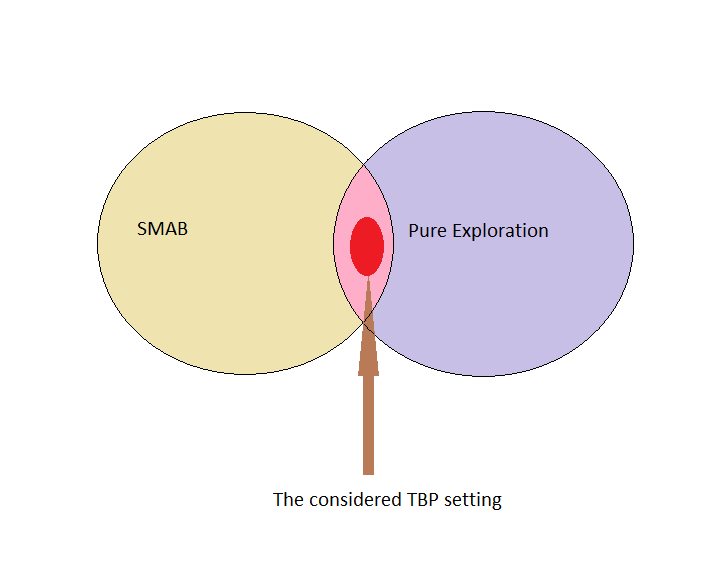
\includegraphics[scale=0.7]{Chapter4/img/connection_TBP.png}
\caption{Connection between TBP, Pure Exploration and SMAB}
\label{fig:con}
\end{figure}

\subsubsection{Challenges in the TBP seeting}

Further, if we look closely into the TBP setting we will see that there are several similarities between the challenges in SMAB setting and the TBP setting. These challenges are as follows:-

\begin{enumerate}
\item The more closer an arm’s expected reward mean ($r_i$) is  to $\tau$, the more harder is the problem. This stems from the fact that it becomes increasingly difficult to discriminate between the arms lying above and below $\tau$.
\item Lesser the budget $T$, the more harder is the problem. This is because there are lesser number of pulls available and so the number of samples collected tends to be low.
\item The higher the variance of an arm’s reward distribution $D_i$, the more harder is the problem. This is similar to the first case as it becomes harder to discriminate between the arms lying close to the threshold.
\end{enumerate}

In the theoretical section in Chapter \ref{chap:tbandit2} we will try to characterize this hardness and give guarantees that are almost optimal.


\section{Related Work in Thresholding Bandits}
\label{tbandit:prevResAPT}

\begin{algorithm}[!h]
\caption{APT}
\label{alg:apt}
\begin{algorithmic}
\State {\bf Input:} Time horizon $T$, threshold $\tau$, tolerance factor $\epsilon\geq 0$
\State Pull each arm once
\State \For{$t=K+1,..,T$}
\State Pull arm $j\in\argmin_{i\in A}\big\lbrace \left(|\hat{r}_{i} - \tau | + \epsilon\right)\sqrt{n_i}\big\rbrace$ and observe the reward for arm $j$.
\EndFor
\State \textbf{Output:} $\hat{S}_{\tau}=\lbrace i: \hat{r}_{i}\geq \tau \rbrace$.
\end{algorithmic}
\end{algorithm}


In the latest work of \citet{locatelli2016optimal} Anytime Parameter-Free Thresholding (APT) algorithm comes up with an improved anytime guarantee than CSAR for the thresholding bandit problem.	


\section{Summary}
\label{tbandit:conc}
In this chapter, we looked at the pure exploration MAB and thresholding bandit (TBP) setting which is a special case of combinatorial pure exploration MAB. We then looked at the various state-of-the-art algorithms in the literature for the pure-exploration setting and discussed the advantages and disadvantages of them. Then we looked at the latest algorithm for the TBP setting. The expected loss that has been proven for the said algorithms have also been discussed at length and their exploration parameters have also been compared against each other. In the next chapter, we provide our solution to this TBP setting which uses variance estimation to find the set of arms above the threshold.


%%%%%%%%%%%%%%%%%%%%%%%%%%%%%%%%%%%%%%%%%%%%%%%%%%%%%%%%%%%%%%%




%%%%%%%%%%%%%%%%%%%%%%%%%%%%%%%%%%%%%%%%%%%%%%%%%%%%%%%%%%%%%%%
\clearemptydoublepage
\chapter{Augmented UCB for Thresholding Bandit Problem}
\label{chap:tbandit2}

\section{Introduction}
\label{tbandit:intro2}
In this chapter we look at the Augmented-UCB (AugUCB) algorithm for a fixed-budget version of the thresholding bandit problem (TBP), where the objective is to identify a set of arms whose expected mean is above a threshold. A key feature of AugUCB is that it uses both mean and variance estimates to eliminate arms that have been sufficiently explored; to the best of our knowledge this is the first algorithm to employ such an approach for the considered TBP.  Theoretically, we obtain an upper bound on the loss (probability of mis-classification) incurred by AugUCB. Although UCBEV in literature provides a better guarantee, it is important to emphasize that UCBEV has access to problem complexity (whose computation requires arms' mean and variances), and hence is not realistic in practice; this is in contrast to AugUCB whose implementation does not require any such complexity inputs. We conduct extensive simulation experiments to validate the performance of AugUCB. Through our simulation work, we establish that AugUCB, owing to its utilization of variance estimates, performs significantly better than the state-of-the-art APT, CSAR and other non variance-based algorithms.


\section{Our Contributions}
\label{tbandit:contribution}
We propose the Augmented UCB (AugUCB) algorithm for the fixed-budget setting of a specific combinatorial, pure-exploration, stochastic MAB called the thresholding bandit problem.
%In this paper we propose AugUCB algorithm for the fixed-budget, comp thresholding bandit problem.
 AugUCB essentially combines the approach of UCB-Improved, CCB \citep{liu2016modification} and APT algorithms. Our algorithm takes into account the empirical variances of the arms along with mean estimates; to the best of our knowledge this is the first variance-based algorithm for the considered TBP. 
Thus, we also address an open problem discussed in \cite{auer2010ucb} of designing an algorithm that can eliminate arms based on variance estimates. In this regard, note that both CSAR and APT are not variance-based algorithms. 

\begin{table}[b]
\caption{AugUCB vs.\ State of the art}
\label{tab:regret-bds}
\begin{center}
\begin{tabular}{|p{2.3cm}|p{8.4cm}|}
% \toprule
\hline
Algorithm  & Upper Bound on Expected Loss \\
% \midrule
\hline
\hline
AugUCB      &$ \exp\left(- \dfrac{T}{4096 \log(K\log K)H_{\sigma,2}} + \log\left(2KT\right) \right) $ \\
\hline
\hline
UCBEV		&$\exp\left(-\dfrac{1}{512}\frac{T-2K}{H_{\sigma,1}} + \log\left(6KT\right)\right)$ \\
%\midrule
\hline
\hline
APT         &$\exp\left(-\dfrac{T}{64 H_1}+2\log((\log(T)+1)K)\right)$ \\
% \midrule
\hline
\hline
CSAR		&$\exp\left(-\dfrac{T-K}{72\log(K)H_{CSAR,2}}+2\log(K)\right)$ \\
%\midrule
\hline

%\bottomrule
\end{tabular}
\end{center}
\end{table}

Our theoretical contribution comprises 
 proving an upper bound on the expected loss incurred by AugUCB (Theorem~\ref{tbandit:Result:Theorem:1}).
In Table \ref{tab:regret-bds} we compare the upper bound on the losses incurred by the various algorithms, including AugUCB. The terms $H_1, H_2$, $H_{CSAR,2}, H_{\sigma,1}$ and $H_{\sigma,2}$ represent various problem complexities, and are as defined in Section~\ref{tbandit:results}. From Section~\ref{tbandit:results} we note that, for all $K\ge8$, we have
\begin{align*}
\log\left(K\log K\right) H_{\sigma,2} > \log(2K) H_{\sigma,2} \ge H_{\sigma,1}.
\end{align*}
%; relation between these quantities are also given in Section~\ref{results} 
%The term containing $H_{\sigma,2}$ is comparable to the similar terms (containing $H_{\sigma,1}$) for the error probability of GapE-V \cite{gabillon2011multi} algorithm which we modify to perform in the TBP problem and name it as UCBEV.
Thus, it follows that the upper bound for UCBEV is better than that for AugUCB.
 %The error probability of UCBEV for single bandit multi-armed case is given in Table \ref{tab:regret-bds}. We see that $\log(\frac{3}{16} K\log K) H_2^{\sigma} > \log(2K) H_2^{\sigma} \ge H_1^{\sigma}$ and hence our algorithm is weaker with respect to UCBEV for single  multi-armed bandit scenario.
 However, implementation of UCBEV algorithm requires $H_{\sigma,1}$ as input, whose computation is not realistic in practice. In contrast, our AugUCB algorithm requires no such complexity factor as input. 
%Theoretically, we can compare the first term (containing $H_2$) of our expected loss and see that for all $K\geq 4$, $ H_2 \log(\frac{3}{16} K\log K) > (\log K)H_{CSAR,2}\geq H_1 $ and hence our result is weaker than CSAR and APT.

Proceeding with the comparisons, we emphasize that the upper bound for  AugUCB is, in fact, not comparable with that of APT and CSAR; this is because the complexity term $H_{\sigma,2}$ is not explicitly comparable with either $H_1$ or $H_{CSAR,2}$. However, through extensive simulation experiments we find that AugUCB significantly outperforms both APT, CSAR and other non variance-based algorithms. AugUCB also outperforms UCBEV under explorations where non-optimal values of $H_{\sigma,1}$  are used. In particular, we consider experimental scenarios comprising large number of arms, with the variances of arms in $S_\tau$ being large. AugUCB, being variance based, exhibits superior performance under these settings.  
%


%Empirically we show that for a large number of arms when the variance of the arms lying above $\tau$ are high, our algorithm performs better than all other algorithms, except the algorithm UCBEV which has access to the underlying problem complexity and also is a variance-aware algorithm. 
%
%AugUCB requires one input parameter and the exact choice for the parameter is derived in Theorem \ref{Result:Theorem:1}. Also, unlike SAR or CSAR, AugUCB does not have explicit accept or reject sets rather the arm elimination condition simply removes arm(s) if it is sufficiently sure that the mean of the arms are very high or very low about the threshold based on mean and variance estimation thereby re-allocating the remaining budget among the surviving arms. This although is a tactic similar to SAR or CSAR, but here at any round, an arbitrary number of arms can be accepted or rejected thereby improving upon SAR and CSAR which accepts/rejects one arm in every round. Also their round lengths are non-adaptive and they pull all the arms equal number of times in each round. 
%At every timestep AugUCB pulls the arm that minimizes thereby making this an anytime algorithm whereby we need not finish every round. 
%Irrespective of this case AugUCB also employs elimination of arms based on mean estimation only and is the first such algorithm which uses elimination by both mean and variance estimation simultaneously.

%The remainder of the paper is organized as follows. In section \ref{tbandit:algorithm} we present our AugUCB algorithm. 
%Section \ref{tbandit:results} contains our main theorem on expected loss, while section \ref{tbandit:expt} contains simulation experiments. We finally draw our conclusions in section \ref{tbandit:conclusion}.
%in section \ref{notation} we introduce the notations and the


\section{Augmented-UCB Algorithm}
\label{tbandit:algorithm}
\textbf{The Algorithm:} The Augmented-UCB (AugUCB) algorithm is presented in Algorithm~\ref{alg:augucb}.
AugUCB is essentially based on the arm elimination method of the UCB-Improved \cite{auer2010ucb}, but adapted to the thresholding bandit setting proposed in \cite{locatelli2016optimal}. However, unlike the UCB improved (which is based on mean estimation) our algorithm employs \emph{variance estimates} (as in \cite{audibert2009exploration}) for arm elimination; to the best of our knowledge this is the first variance-aware  algorithm for the thresholding bandit problem. Further, we allow for arm-elimination at each time-step, which is in contrast to the earlier work (e.g., \cite{auer2010ucb,chen2014combinatorial}) where the arm elimination task is deferred to the end of the respective exploration rounds. The details are presented below.

% In algorithm \ref{alg:augucb}, hence referred to as AugUCB, we have two exploration parameters, $\rho_{\mu}$ and $\rho_v$ which are the arm elimination parameters. $\psi_{m}$ is the exploration regulatory factor. 
%The main approach is based on the UCB-Improved algorithm with modifications suited for the thresholding bandit problem. 
The active set $B_{0}$ is initialized with all the arms from $\mathcal{A}$. We divide the entire budget $T$ into rounds/phases like in UCB-Improved, CCB, SAR and CSAR. At every time-step AugUCB checks for arm elimination conditions, while updating parameters at the end of each round. As suggested by \cite{liu2016modification} to make AugUCB to overcome too much early exploration, we no longer pull all the arms equal number of times in each round. Instead, we choose an arm in the active set $B_m$ that minimizes $(|\hat{r}_{i} - \tau |-2s_i)$ where 
%$\min_{i\in B_{m}}\big\lbrace |\hat{r}_{i} - \tau | - 2\sqrt{\frac{\rho_v\psi_m \hat{V}_{i} \log ( T \epsilon_{m})}{4 n_{i}} + \frac{\rho_v\psi_m \log{( T\epsilon_{m})}}{4 n_{i}}} \big\rbrace $
\begin{small}
\begin{align*}
s_i & = \sqrt{\frac{\rho\psi_m (\hat{v}_{i}+1) \log ( T \epsilon_{m})}{4 n_{i}}} %+ \frac{\rho\psi_m \log{( T\epsilon_{m})}}{4 n_{i}}}.
\end{align*}
\end{small} 
with $\rho$ being the arm elimination parameter and $\psi_{m}$ being the exploration regulatory factor.
%  in the active set $B_{m}$. 
The above condition ensures that an arm closer to the threshold $\tau$ is pulled; 
%and with suitable choice of $\rho_{\mu}$ and $\rho_v$ we can fine tune the exploration. 
parameter $\rho$ can be used to fine tune the elimination interval.
The choice of exploration factor, $\psi_m$,
% $\psi_m=\frac{T\epsilon_m}{(\log(\frac{3}{16} K\log K))^{2}}$ 
comes directly from \cite{audibert2010best} and \cite{bubeck2011pure} where it is  stated that in pure exploration setup, the exploring factor must be linear in $T$ (so that an exponentially small probability of error is achieved) rather than being logarithmic in $T$ (which is more suited for minimizing cumulative regret).

\begin{algorithm}[t!]
\caption{AugUCB}
\label{alg:augucb}
\begin{algorithmic}
\State {\bf Input:} Time budget $T$; parameter $\rho$; 
% $\rho_{\mu}$, $\rho_v$ 
  threshold $\tau$
\State {\bf Initialization:} $B_{0}=\mathcal{A}$; $m=0$; $\epsilon_{0}=1$;
\begin{small}
\begin{align*}
M&=\left\lfloor \frac{1}{2}\log_{2} \frac{T}{e}\right\rfloor; 
\hspace{2mm}\psi_{0}=\frac{T\epsilon_{0}}{128\Big(\log(\frac{3}{16}K\log K)\Big)^2}; \\
\ell_{0}&=\left\lceil \frac{2\psi_0\log( T\epsilon_{0})}{\epsilon_{0}} \right\rceil;
\hspace{2mm}N_{0}=K\ell_{0}
\end{align*}
\end{small}
%$M=\left\lfloor \frac{1}{2}\log_{2} \frac{T}{e}\right\rfloor $,  
%$\psi_{0}=\frac{T\epsilon_{0}}{(\log(\frac{3}{16}K\log K)^2}$,
% $\ell_{0}=\left\lceil \frac{2\psi\log( T\epsilon_{0})}{\epsilon_{0}} \right\rceil$ and 
% $N_{0}=K\ell_{0} $. Pull each arm once.
\State Pull each arm once
\vspace{-2mm}
\State \For{$t=K+1,..,T$}
\State Pull arm $j\in\argmin_{i\in B_{m}}\Big\lbrace |\hat{r}_{i} - \tau | - 2s_{i}\Big\rbrace$
% \State where $s_j=\sqrt{\frac{\rho\psi_{m}\hat{v}_{j}\log{( T\epsilon_{m})}}{4 n_{j}} + \frac{\rho\psi_{m} \log{(T\epsilon_{m})}}{4 n_{j}}}$
\State $t\leftarrow t+1$ 
\vspace{-4mm}
%\ArmElim
%\State For each arm $i \in B_{m}$, remove arm ${i}$ from $B_{m}$ if
%\begin{align*}
%\hat{r}_{i} + c_i  < \tau - c_i \mbox{ or } \hat{r}_{i} - c_i  > \tau + c_i \\
%\text{where $c_i=\sqrt{\frac{\rho_{\mu}\psi_{m}\log{( T\epsilon_{m})}}{2 n_{i}}}$}
%\end{align*}
%\EndArmElim
%\ArmElimV
%\State \For{$i\in B_m$}
%\State For each arm $i \in B_{m}$, remove arm ${i}$ from $B_{m}$ if
\State \For{$i\in B_m$}
\vspace{-4mm}
\State \If{$(\hat{r}_{i} + s_i  < \tau - s_i)$ or $(\hat{r}_{i} - s_i > \tau + s_i)$}
\State $B_m\leftarrow B_m\backslash\{i\}$\hspace{4mm} (Arm deletion)
\EndIf
\EndFor
%\begin{align*}
%\hat{r}_{i} + s_i  < \tau - s_i,\hspace{1mm} \mbox{ or } \hspace{1mm}\hat{r}_{i} - s_i  > \tau + s_i \\
%% \text{where $s_i=\sqrt{\frac{\rho\psi_{m}\hat{v}_{i}\log{( T\epsilon_{m})}}{4 n_{i}} + \frac{\rho\psi_{m} \log{(T\epsilon_{m})}}{4 n_{i}}}$}
%\end{align*}
%\EndFor
%\EndArmElimV
\vspace{-2mm}
\State \If{$t\geq N_{m}$ and $m \leq M$}
%\ResetParam
\State \textbf{Reset Parameters}
\State $\epsilon_{m+1}\leftarrow\frac{\epsilon_{m}}{2}$
\State $B_{m+1} \leftarrow B_{m}$
\State $\psi_{m+1}\leftarrow \frac{T\epsilon_{m+1}}{128(\log(\frac{3}{16}K\log K))^{2}}$
\State $\ell_{m+1}\leftarrow\left\lceil \frac{2\psi_{m+1}\log( T\epsilon_{m+1})}{\epsilon_{m+1}} \right\rceil$
\State $N_{m+1} \leftarrow t + |B_{m+1}|\ell_{m+1}$
\State $m \leftarrow m+1$
%\EndResetParam
\EndIf
\EndFor
\State \textbf{Output:} $\hat{S}_{\tau}=\lbrace i: \hat{r}_{i}\geq \tau \rbrace$.
\end{algorithmic}
\end{algorithm}


%Also because of the said condition, like \cite{liu2016modification} we also claim that AugUCB is an anytime algorithm.



\section{Theoretical Results}
\label{tbandit:results}
% \subsection{Problem Complexity}

Let us begin by recalling the following definitions of the  \emph{problem complexity} as introduced in \cite{locatelli2016optimal}:
\begin{align*}
H_{1} = \sum_{i=1}^{K}\dfrac{1}{\Delta_{i}^{2}} \hspace{1mm}\text{     and }  \hspace{1mm}
H_{CSAR,2} =\min_{i\in \mathcal{A}}\dfrac{i}{{\Delta_{(i)}^{2}}} 
\end{align*}
where $(\Delta_{(i)}: i\in\mathcal{A})$ is obtained by arranging $(\Delta_i:i\in\mathcal{A})$ in an increasing order. Also, from \cite{chen2014combinatorial} we have
\begin{align*}
H_{CSAR,2}=\max_{i\in\mathcal{A}}\frac{i}{\Delta_{(i)}^2}.
\end{align*}
$H_{CSAR,2}$ is the complexity term appearing in the bound for the CSAR algorithm. The relation between the above complexity terms are as follows (see \cite{locatelli2016optimal}):
%
%$H_1$ and $H_2$ is same as the problem complexity defined in \cite{locatelli2016optimal} for the thresholding bandit problem while $H_{CSAR,2}=\max_{i}\frac{i}{\Delta_{(i)}^2}$ is defined in \cite{chen2014combinatorial}. Also we know from \cite{locatelli2016optimal} that,
\begin{align*}
H_{1}\leq \log(2K)H_{2} \mbox{ and }
 H_1 \leq \log(K)H_{CSAR,2}.
\end{align*}

As ours is a variance-aware algorithm, we require $H_{1}^{\sigma}$ (as defined in \cite{gabillon2011multi}) that incorporates reward variances into its expression as given below:
\begin{align*}
 H_{\sigma,1}=\sum_{i=1}^{K}\frac{\sigma_{i}+\sqrt{\sigma_{i}^{2}+(16/3)\Delta_{i}}}{\Delta_{i}^{2}}.
\end{align*}
Finally, analogous to $H_{CSAR,2}$, in this paper we introduce the complexity term $H_{\sigma,2}$, which is given by
%and $H_{2}^{\sigma}$ (introduced in this paper) as,
\begin{align*}
%& H_{1}^{\sigma}=\sum_{i=1}^{K}\frac{\sigma_{i}+\sqrt{\sigma_{i}^{2}+(16/3)\Delta_{i}}}{\Delta_{i}^{2}}\\
H_{\sigma,2}=\max_{i\in \mathcal{A}} \frac{i}{\tilde{\Delta}_{(i)}^{2}}%& H_{2}^{\sigma}=\min_{i\in \mathcal{A}} i\frac{12\sigma_{(i)}^{2} + \Delta_{(i)}}{12\Delta_{(i)}^{2}}
\end{align*}
where $\tilde{\Delta}_{i}^{2}=\frac{\Delta_{i}^{2}}{\sigma_{i}+\sqrt{\sigma_{i}^{2}+(16/3)\Delta_{i}}}$, and $(\tilde{\Delta}_{(i)})$ is an increasing ordering of $(\tilde{\Delta}_{i})$. Following the results in \cite{audibert2010best}, we can show that
\begin{align*}
H_{\sigma,2}\le H_{\sigma,1}\le\overline{\log}(K) H_{\sigma,2} \le \log(2K) H_{\sigma,2}.
\end{align*}


%Similar to the relation between $H_1$ and $H_2$, it can be shown that
%%which also gives us that 
%$H_{2}^{\sigma} \leq H_{1}^{\sigma} \leq \log(2K) H_{2}^{\sigma}$.
%
%Also, from \cite{audibert2010best} we know that,
%\begin{align*}
%\sum_{i=1}^{K}\tilde{\Delta}_{i}^{-2} = \tilde{\Delta}_{(2)}^{-2} + \sum_{i=2}^{K}\frac{1}{i}i\tilde{\Delta}_{(i)}^{-2} &\leq \bar{\log K}\min_{i}i\tilde{\Delta}_{(i)}^{-2}\\
%& \leq \log(2K) H_{2}^{\sigma}, \text{ as $\bar{\log K} \leq \log(2K)$}
%\end{align*}


%\subsection{Theorem 1}
Our main result is summarized in the following theorem where we prove an  upper bound on the expected loss. 
\begin{theorem}
\label{tbandit:Result:Theorem:1}
For $K\geq 4$ and
%with $\rho_{\mu}=\frac{1}{8}$ and 
$\rho={1}/{3}$,
the expected loss of the AugUCB algorithm is given by,
%\begin{small}
\begin{align*}
\E[\Ls(T)]
%\exp\bigg( -\frac{T\log (2 K\sqrt{\log K})}{2H_2 K (\log K)^{3/2}} + \log\bigg(K\big(\log_2\frac{T}{e}+1\big)\bigg)\bigg)\\
%& + \exp\bigg(- \frac{5T\log ( K\sqrt{\log K})}{H_{2}^{\sigma} K(\log K)^{3/2}}  + \log\bigg(K\big(\log_2\frac{T}{e}+1\big)\bigg)\bigg).
& \leq 2KT
% \bigg\lbrace\exp\bigg( -\frac{T}{ 64 H_2 a}\bigg)
% + 2
 \exp\bigg(- \frac{T}{4096 \log( K\log K) H_{\sigma,2}} \bigg).
 %\bigg\rbrace
\end{align*}
%where $a=\log(\frac{3}{16} K\log K)$.
%\end{small}
%For every $0<\eta <1$ and $\gamma > 1$, there exists time $t$ such that for all $T>t$ the simple regret of AugUCB is upper bounded by,
%\begin{small}
%\begin{align*}
%& SR_{AugUCB} \leq \sum_{i=1}^{K} \Delta_{i}\bigg\lbrace \exp\bigg(-4\rho\log (\psi T\frac{\Delta_{i}^{4}}{16\rho^{2}})-\dfrac{c_{0}\sqrt{T}}{16\rho H_{2}}\\
%& + \log \big( 16\gamma C_1\log_{2}\dfrac{T}{e} \big) \bigg) + \exp\bigg(- \dfrac{3\rho_v}{2} \bigg(\dfrac{2\sigma_{i}^{2}+\Delta_{i}+2}{6\sigma_{i}^{2}+\Delta_{i}}\bigg)\log(\psi T\frac{\Delta_{i}^{4}}{16\rho_{v}^{2}})\\
%& -\dfrac{c_{0}\sqrt{T}}{16\rho_v H_{2}} + \log\big ( 32\gamma C_2\log_{2}\dfrac{T}{e} \big)  \bigg)\bigg\rbrace
%\end{align*}
%\end{small}
%with probability at least $1-\eta$, where $c_{0}>0$ is a constant and $C_1=\dfrac{K\rho\log (\psi T \frac{\Delta_{i}^{4}}{16\rho^{2}})}{T\Delta_{i}^{2}}$ and $C_2= \dfrac{K\rho_v\log (\psi T \frac{\Delta_{i}^{4}}{16\rho_{v}^{2}})}{T\Delta_{i}^{2}}$.
\end{theorem}

\begin{proof}
The proof comprises of two modules. In the first module we investigate the necessary conditions for arm elimination within a specified number of rounds, which is motivated by the technique in \cite{auer2010ucb}. Bounds on the arm-elimination probability is then obtained; however, since we use variance estimates, we invoke the Bernstein inequality (as in \cite{audibert2009exploration}) rather that the Chernoff-Hoeffding bounds (which is appropriate for the UCB-Improved \citep{auer2010ucb}). In the second module, as in \cite{locatelli2016optimal}, we first define a favourable event that will yield an upper bound on the expected loss. Using union bound, we then incorporate the result from module-1 (on the arm elimination probability), and finally derive the result through a series of simplifications.
%In the final module we conclude by combining the results for the first two modules. 
The details are as follows. 


\textbf{Arm Elimination:} Recall the notations used in the algorithm, Also, for each arm $i\in\mathcal{A}$, define $m_{i}=\min\left\lbrace m| \sqrt{\rho\epsilon_{m}}<\frac{\Delta_{i}}{2}\right\rbrace$. In the $m_i$-th round, whenever $n_i=\ell_{m_i}\ge\frac{2\psi_{m_i}\log{(T\epsilon_{m_{i}})}}{\epsilon_{m_{i}}}$, we obtain (as $\hat{v}_i\in[0,1]$)
%
%\begin{align*}
%s_{i}&=\sqrt{\dfrac{\rho \psi_{m_i} \hat{v}_{i} \epsilon_{m_{i}}\log ( T\epsilon_{m_{i}})}{4 n_{i}} + \dfrac{\rho \psi_{m_i}\log{( T\epsilon_{m_{i}})}}{4 n_{i}}} \\
%&\leq \sqrt{\dfrac{\rho\psi_{m_i} \epsilon_{m_{i}}\log ( T\epsilon_{m_{i}})}{4*2 \log(\psi_{m_i} T\epsilon_{m_{i}})} + \dfrac{\rho\psi_{m_i}\epsilon_{m_{i}} \log{( T\epsilon_{m_{i}})}}{4*2\psi_{m_i} \log( T\epsilon_{m_{i}})} } \text{, as }\hat{V}_{i}\in [0,1].\\
%& \leq \sqrt{\dfrac{\rho_v \epsilon_{g_{i}}}{8} + \dfrac{\rho_v \epsilon_{g_{i}}}{8} } \leq \dfrac{\sqrt{\rho_v \epsilon_{g_{i}}}}{2}< \dfrac{\Delta_{i}}{4} \text{, as }\rho_v\in (0,1].
%%& \leq \sqrt{\rho_v \epsilon_{g_{i}+1}} < \dfrac{\Delta_{i}}{4} \text{, as }\rho_v\in (0,1].
%\end{align*}
%
\begin{align}
\label{si_bound_equn}
s_i 
&\le \sqrt{\frac{\rho(\hat{v}_i+1)\epsilon_{m_i}}{8}}
% +\frac{\rho\epsilon_{m_i}}{8}}
  \le \frac{\sqrt{\rho\epsilon_{m_i}}}{2} < \frac{\Delta_i}{4}.
\end{align}

First, let us consider a bad arm $i\in\mathcal{A}$ (i.e., $r_i<\tau$). We note that, in the $m_i$-th round  whenever 
$\hat{r}_i \le r_i +2s_i$, then arm $i$ is eliminated as a bad arm. This is easy to verify as follows: using (\ref{si_bound_equn}) we obtain,
\begin{align*}
\hat{r}_{i}\leq r_{i} + 2s_{i} 
%&= r_{i} + 4s_{i} - 2s_{i} \\
< r_{i} + \Delta_{i} - 2s_{i} 
= \tau - 2s_{i} % \geq \tau + s_{i}
\end{align*}
which is precisely one of the elimination conditions in Algorithm~\ref{alg:augucb}. Thus, the probability that a bad arm is not eliminated correctly in the $m_i$-th round (or before) is given by

%%%%%%%%%%%%%%%%% Favorable event is defined here
%We note that in the $g_i$-th round arm $i$ can be pulled no more than $\ell_{g_i}$ number of times. 
%
%
%According to the algorithm, the number of rounds is $m=\lbrace 0,1,2,.. M\rbrace $ where $M=\bigg\lfloor \frac{1}{2}\log_{2} \frac{T}{e}\bigg\rfloor$. So, $\epsilon_{m}\geq 2^{-M}\geq \sqrt{\frac{e}{T}}$. Also each round $m$ consists of $|B_{m}|\ell_{m}$ timesteps where $\ell_{m} = \left\lceil\frac{2\psi_{m}\log( T \epsilon_{m})}{\epsilon_{m}}\right\rceil$, $B_{m}$ is the set of all surviving arms and let $a=(\log(\frac{3}{16} K\log K))$.
%
%
%Let $c_{i} = \sqrt{\frac{\rho_{\mu}\psi_{m} \log{(T\epsilon_{m})}}{2 n_{i}}}$ denote the confidence interval, where $n_{i}$ is the number of times an arm $i$ is pulled. Let $\mathcal{A}^{'}=\lbrace i\in \mathcal{A}|\Delta_{i}\geq b\rbrace$, for $b\geq \sqrt{\frac{e}{T}}$. Define $m_{i}=\min\lbrace m| \sqrt{\rho_{\mu}\epsilon_{m}}<\frac{\Delta_{i}}{2}\rbrace$.
%% Let $m_{i}$ be the minimum round such that an arm $i$ gets eliminated such that. 
%
%% Let $s_{i}=\sqrt{\frac{\rho_v\psi_{g} \hat{V_{i}} \log{( T\epsilon_{g})}}{4 n_{i}} + \frac{\rho_v\psi_{g} \log{( T\epsilon_{g})}}{4 n_{i}}}$ and 
%% $g_{i}$ be the minimum round that an arm $i$ gets eliminated such that $g_{i}=min\lbrace g| \sqrt{\rho_{v}\epsilon_{g}}<\frac{\Delta_{i}}{2}\rbrace$. 
%%In this proof sub-optimal arms refer to the arms whose $r_{i}$ is lower than the threshold $\tau$.
%
%%At the end of any round $\max\lbrace m_{i},g_{i}\rbrace$, for any arm $i$, two cases are possible.
%
%Let $\xi_{1}$ and $\xi_{2}$ be the favorable event such that,
%\begin{align*}
%\xi_{1}&=\bigg\lbrace \forall i\in \mathcal{A}, \forall m=0,1,2,..,M: |\hat{r_i} - r_i| \leq 2c_i\bigg\rbrace\\
%\xi_{2}&=\bigg\lbrace \forall i\in \mathcal{A}, \forall m=0,1,2,..,M: |\hat{r_i} - r_i| \leq  2s_i\bigg\rbrace
%\end{align*}
%
%So, $\xi_{1}$ and $\xi_{2}$ signifies the event any arm $i$ will get eliminated from $B_m$.
%%%%%%%%%%%%%%%%%%%%%%







%%%%%%%%%%%%%%%%%
%\subsubsection{\textit{Arm i is not eliminated on or before round $\max\lbrace m_{i},g_{i}\rbrace$}}
%
%For any arm $i$, if it is eliminated from active set $B_{m_{i}}$ then one of the below two events has to occur,
%%\begin{small}
%\begin{align}
%\hat{r}_{i} + c_{i} < \tau - c_{i}, \label{eq:armelim-casea}\\
%\hat{r}_{i} - c_{i} > \tau + c_{i}, \label{eq:armelim-caseb}
%\end{align}
%%\end{small}
%For (\ref{eq:armelim-casea}) we can see that it eliminates arms that have performed poorly and removes them  from $B_{m_{i}}$. Similarly, (\ref{eq:armelim-caseb}) eliminates arms from $B_{m_{i}}$ that have performed very well compared to threshold $\tau$.
%
%%Each round consists of $|B_{m_{i}}|\ell_{m_{i}}$ timesteps. 
%In the $m_{i}$-th round an arm $i$ can be pulled no more than $\ell_{m_{i}}$ times. So when $n_{i}=\ell_{m_{i}}$, putting the value of $\ell_{m_{i}}\ge\frac{2\psi_{m_i}\log{( T\epsilon_{m_{i}})}}{\epsilon_{m_{i}}}$ in $c_{i}$ we get, 
%%\begin{small}
%\begin{align*}
%c_{i}
%&=\sqrt{\frac{\rho_{\mu}\psi_{m_i}\epsilon_{m_{i}}\log ( T\epsilon_{m_{i}})}{2 n_{i}}}
%\le\sqrt{\frac{\rho_{\mu}\psi_{m_i}\epsilon_{i}\log ( T\epsilon_{m_{i}})}{2*2 \psi_{m_i} \log( T\epsilon_{m_{i}})}}\\
%& \le\frac{\sqrt{\rho_{\mu}\epsilon_{m_{i}}}}{2}
%% % \leq \sqrt{\rho_{\mu}\epsilon_{m_{i}+1}} 
%< \frac{\Delta_{i}}{4} \text{, as }\rho_{\mu}\in (0,1].
%\end{align*}
%%\end{small}
%Again, for ${i} \in \mathcal{A}^{'}$ for the  elimination condition in (\ref{eq:armelim-casea}), 
%%\begin{small}
%%\begin{align*}
%%\hat{r}_{i} + c_{i}&\leq r_{i} + 2c_{i} = r_{i} + 4c_{i} - 2c_{i} \\
%%&< r_{i} + \Delta_{i} - 2c_{i} = \tau -2c_{i} \leq \tau - c_{i}
%%\end{align*}
%%\end{small}
%%\begin{small}
%\begin{align*}
%\hat{r}_{i} &\leq r_{i} + 2c_{i} = r_{i} + 4c_{i} - 2c_{i} \\
%&< r_{i} + \Delta_{i} - 2c_{i} = \tau -2c_{i}.
%\end{align*}
%%\end{small}
%Similarly, for ${i} \in \mathcal{A}^{'}$ for the  elimination condition in (\ref{eq:armelim-caseb}), 
%%\begin{small}
%\begin{align*}
%\hat{r}_{i} &\geq r_{i} - 2c_{i} = r_{i} - 4c_{i} + 2c_{i} \\
%&> r_{i} - \Delta_{i} + 2c_{i}= \tau + 2c_{i}.
%\end{align*}
%%\end{small}
%
%
%%Now, arm elimination condition is being checked at every timestep, in the $m_{i}$-th round as soon as $n_{i}=\ell_{m_{i}}$, arm $i$ gets eliminated. 
%Applying Chernoff-Hoeffding bound and considering independence of complementary of the event in (\ref{eq:armelim-casea}),
%%\begin{small}
%\begin{align*}
%%\mathbb{P}\lbrace\hat{r}_{i}\geq r_{i} - 2c_{i}\rbrace &\leq exp(-2(\tau + 2c_{i})^{2}n_{i})\\
%&\mathbb{P}\lbrace\hat{r}_{i}> r_{i} + 2c_{i}\rbrace \leq \exp(-4 c_{i}^{2}n_{i})\\
%&\leq \exp(-8 * \dfrac{\rho_{\mu}\psi_{m_i}\log ( T\epsilon_{m_{i}})}{2 n_{i}} *n_{i})\\
%&\leq \exp\big(-4\rho_{\mu}\psi_{m_i}\log ( T\epsilon_{m_{i}})\big)\\
%&\leq \exp\left(-\rho_{\mu}\frac{T\epsilon_{m_{i}}}{32 a^2}\log ( T\epsilon_{m_{i}})\right),\\
%&\text{putting the value of $\psi_{m_i}=\frac{T\epsilon_{m_i}}{128(\log(\frac{3}{16} K\log K))^{2}}$}
%\end{align*}
%%\end{small}
%Similarly for the condition in (\ref{eq:armelim-caseb}), $\mathbb{P}\lbrace\hat{r}_{i}< r_{i} - 2c_{i}\rbrace\leq \exp\left(-\frac{T\rho_{\mu}\epsilon_{m_{i}}}{32 a^2 }\log ( T\epsilon_{m_{i}})\right)$.
%
%Summing the above two expressions, the probability that arm ${i}$ is not eliminated on or before $m_{i}$-th is $\left(2\exp\left(-\frac{T\rho_{\mu}\epsilon_{m_{i}}}{32 a^2 }\log ( T\epsilon_{m_{i}})\right)\right)$. 
%%%%%%%%%%%%%%%%%%%%%

%%%%%%%%%%%%
%Again for any arm $i$, if it is eliminated from active set $B_{g_{i}}$ then the below two events have to come true,
%%\begin{small}
%\begin{align}
%\hat{r}_{i} + s_{i} < \tau - s_{i}, \label{eq:armelim-var-casea}\\
%\hat{r}_{i} - s_{i} > \tau + s_{i}, \label{eq:armelim-var-caseb}
%\end{align}
%%\end{small}
%%
%% For \ref{eq:armelim-var-casea} we can see that it eliminates arms that have performed poorly and removes them them from $B_{g_{i}}$. Similarly, \ref{eq:armelim-var-caseb} eliminates arms from $B_{g_{i}}$ that have performed very well compared to threshold $\tau$.
%%But, we know that $\epsilon_{m_{i}}=\epsilon_{g_{i}}$ and round consist of $|B_{g_{i}}|\ell_{g_{i}}$ timesteps. 
%In the $g_{i}$-th round an arm $i$ can be pulled no more than $\ell_{g_{i}}$ times. So when $n_{i}=\ell_{g_{i}}$, putting the value of $\ell_{g_{i}}\ge\frac{2\psi_{m_i}\log{( T\epsilon_{g_{i}})}}{\epsilon_{g_{i}}}$ in $s_{i}$ we get, 
%%\begin{small}
%\begin{align*}
%s_{i}&=\sqrt{\dfrac{\rho_v \psi_{g_i} \hat{V}_{i} \epsilon_{g_{i}}\log ( T\epsilon_{g_{i}})}{4 n_{i}} + \dfrac{\rho_v \psi_{g_i}\log{( T\epsilon_{g_{i}})}}{4 n_{i}}} \\
%&\leq \sqrt{\dfrac{\rho_v\psi_{g_i} \epsilon_{g_{i}}\log ( T\epsilon_{g_{i}})}{4*2 \log(\psi_{g_i} T\epsilon_{g_{i}})} + \dfrac{\rho_v \psi_{g_i}\epsilon_{g_{i}} \log{( T\epsilon_{g_{i}})}}{4*2\psi_{g_i} \log( T\epsilon_{g_{i}})} } \text{, as }\hat{V}_{i}\in [0,1].\\
%& \leq \sqrt{\dfrac{\rho_v \epsilon_{g_{i}}}{8} + \dfrac{\rho_v \epsilon_{g_{i}}}{8} } \leq \dfrac{\sqrt{\rho_v \epsilon_{g_{i}}}}{2}< \dfrac{\Delta_{i}}{4} \text{, as }\rho_v\in (0,1].
%%& \leq \sqrt{\rho_v \epsilon_{g_{i}+1}} < \dfrac{\Delta_{i}}{4} \text{, as }\rho_v\in (0,1].
%\end{align*}
%%\end{small}
%
%Again, for ${i} \in \mathcal{A}^{'}$ for the elimination condition in (\ref{eq:armelim-var-casea}),
%%\begin{small}
%\begin{align*}
%\hat{r}_{i} &\leq r_{i} + 2s_{i} = r_{i} + 4s_{i} - 2s_{i} \\
%&< r_{i} + \Delta_{i} - 2s_{i} = \tau -2s_{i} % \leq \tau - s_{i}
%\end{align*}
%%\end{small} 
%
%
%Also, for ${i} \in \mathcal{A}^{'}$ for the elimination condition in (\ref{eq:armelim-var-caseb}), 
%%\begin{small}
%\begin{align*}
%\hat{r}_{i}&\geq r_{i} - 2s_{i} = r_{i} - 4s_{i} + 2s_{i} \\
%&> r_{i} - \Delta_{i} + 2s_{i}\geq \tau + 2s_{i} % \geq \tau + s_{i}
%\end{align*}
%%\end{small}
%%%%%%%%%%%%%%%%


%Since, arm elimination condition is being checked at every timestep, in the $g_{i}$-th round as soon as $n_{i}=\ell_{g_{i}}$, arm $i$ gets eliminated. 
% Applying Bernstein inequality and considering independence of complementary of the event in (\ref{eq:armelim-var-casea}),
%\begin{small}
\noindent
\begin{align}
\mathbb{P}(\hat{r}_{i}> r_{i} + 2s_{i})
% &= \mathbb{P}\bigg( \hat{r}_{i} > r_{i}+ 2\sqrt{\dfrac{\rho\psi_{m_i} \hat{v}_{i}\log( T\epsilon_{m_{i}}) + \rho\psi_{m_i} \log{( T\epsilon_{m_{i}})}}{4n_{i}} } \bigg)\nonumber\\
&\leq \mathbb{P}\left( \hat{r}_{i} > r_{i}+ 2\bar{s}_i\right)  % \label{eq:prob_eq1}\\ 
+ \mathbb{P}\left( \hat{v}_{i}\geq \sigma_{i}^{2}+\sqrt{\rho\epsilon_{m_{i}}}\right)\label{eq:prob_eq2}
\end{align}
where 
\begin{align*}
\bar{s}_i=\sqrt{\dfrac{\rho\psi_{m_i} (\sigma_{i}^{2}+\sqrt{\rho\epsilon_{m_{i}}} + 1)\log( T\epsilon_{m_{i}})}{4n_{i}}}
\end{align*}
%\end{small}
Note that, substituting $n_i=\ell_{m_i}\ge \frac{2\psi_{m_i}\log{(T\epsilon_{m_{i}})}}{\epsilon_{m_{i}}}$, $\bar{s}_i$ can be simplified to obtain,
\begin{align}
2\bar{s}_i
% &\le 2\sqrt{\dfrac{\rho\psi_{m_i} (\sigma_{i}^{2}+\sqrt{\rho\epsilon_{m_{i}}})\log( T\epsilon_{m_{i}})}{\frac{8\psi_{m_i}\log( T \epsilon_{m_{i}})}{\epsilon_{m_{i}}}} }
%+ \dfrac{\rho\psi_{m_i} \log{( T\epsilon_{m_{i}})}}{\frac{8\psi_{m_i}\log( T \epsilon_{m_{i}})}{\epsilon_{m_{i}}}}}
\leq \dfrac{\sqrt{\rho\epsilon_{m_{i}}(\sigma_{i}^{2}+\sqrt{\rho\epsilon_{m_{i}}} + 1)}}{2}\leq \sqrt{\rho \epsilon_{m_{i}}}.
\label{si_bar_equn}
\end{align}

%Now, we know that in the $g_{i}$-th round,
%%\begin{small}
%\begin{align*}
%& 2\sqrt{\dfrac{\rho_v\psi_{g_i} [\sigma_{i}^{2}+\sqrt{\rho_{v}\epsilon_{g_{i}}}]\log( T\epsilon_{g_{i}})}{4n_{i}} + \dfrac{\rho_v\psi_{g_i}  \log{(T\epsilon_{g_{i}})}}{4 n_{i}}}\\ &\leq  2\sqrt{\dfrac{\rho_v\psi_{g_i} [\sigma_{i}^{2}+\sqrt{\rho_{v}\epsilon_{g_{i}}}]\log( T\epsilon_{g_{i}})}{\frac{8\psi_{g_i}\log( T \epsilon_{g_{i}})}{\epsilon_{g_{i}}}} + \dfrac{\rho_v\psi_{g_i} \log{( T\epsilon_{g_{i}})}}{\frac{8\psi_{g_i}\log( T \epsilon_{g_{i}})}{\epsilon_{g_{i}}}}}\\
%& \leq \dfrac{\sqrt{\rho_v \epsilon_{g_{i}}[\sigma_{i}^{2}+\sqrt{\rho_{v}\epsilon_{g_{i}}} + 1]}}{2}\leq \sqrt{\rho_v \epsilon_{g_{i}}}
%\end{align*}
%%\end{small}
%--------------------

The first term in the LHS of (\ref{eq:prob_eq2}) can be bounded using the Bernstein inequality as below:
\begin{align}
&\mathbb{P}\left( \hat{r}_{i} > r_{i}+ 2\bar{s}_i\right)\nonumber \\
&\le \exp\left(- \dfrac{(2\bar{s}_i)^2 n_i}{2\sigma_i^2+\frac{4}{3}\bar{s}_i}\right)\nonumber \\
& \le \exp\left(- \dfrac{\rho\psi_{m_i} (\sigma_{i}^{2}+\sqrt{\rho\epsilon_{m_{i}}} + 1)\log( T\epsilon_{m_{i}})}{2\sigma_i^2+\frac{2}{3}\sqrt{\rho \epsilon_{m_{i}}}}\right)\nonumber \\
& \overset{(a)}{\leq} \exp\left(- \dfrac{3\rho T\epsilon_{m_i}}{256 a^2} \left(\dfrac{\sigma_{i}^{2}+\sqrt{\rho\epsilon_{m_{i}}}+1}{3\sigma_{i}^{2}+\sqrt{\rho \epsilon_{m_{i}}}}\right) \log( T\epsilon_{m_{i}}) \right) \nonumber \\
&:= \exp(-Z_i) 
\label{lhs1_equn}
\end{align}
where, for simplicity, we have used $\alpha_i$ to denoted the exponent in the inequality $(a)$.
Also, note that $(a)$ is obtained by using  $\psi_{m_i}=\frac{T\epsilon_{m_i}}{128a^{2}}$, where $a=(\log(\frac{3}{16} K\log K))$.
%For the term in (\ref{eq:prob_eq1}), by applying Bernstein inequality, we can write as,
%\begin{small}
%\begin{align*}
%&\mathbb{P}\bigg( \hat{r}_{i}> r_{i} + \bigg(2\sqrt{\frac{\rho_v\psi_{g_i} [\sigma_{i}^{2}+\sqrt{\rho_{v}\epsilon_{g_{i}}} + 1]\log( T\epsilon_{g_{i}})}{4n_{i}}  } \bigg)\bigg)\\
%%%%%%%%%%%%%%%%%%%%%%%%
% &\leq \exp\bigg(- \dfrac{\bigg(2\sqrt{\frac{\rho_v\psi_{g_i} [\sigma_{i}^{2}+\sqrt{\rho_{v}\epsilon_{g_{i}}} +1]\log( T\epsilon_{g_{i}})}{4n_{i}}}\bigg)^{2}n_{i}}{2\sigma_{i}^{2}+\frac{4}{3}\sqrt{\frac{\rho_v\psi_{g_i} [\sigma_{i}^{2}+\sqrt{\rho_{v}\epsilon_{g_{i}}}+1]\log( T\epsilon_{g_{i}})}{4n_{i}}}}\bigg) \\
%%%%%%%%%%%%%%%%%%%%%%%
%&\leq \exp\bigg(- \dfrac{\bigg(\rho_v\psi_{g_i} [\sigma_{i}^{2}+\sqrt{\rho_{v}\epsilon_{g_{i}}} + 1]\log( T\epsilon_{g_{i}})\bigg)}{2\sigma_{i}^{2}+\frac{2}{3}\sqrt{\rho_v \epsilon_{g_{i}}}} \bigg)\\
% &\leq \exp\bigg(- \dfrac{3\rho_v\psi_{g_i}}{2} \bigg(\dfrac{\sigma_{i}^{2}+\sqrt{\rho_{v}\epsilon_{g_{i}}}+1}{3\sigma_{i}^{2}+\sqrt{\rho_v \epsilon_{g_{i}}}}\bigg) \log( T\epsilon_{g_{i}}) \bigg)\\
%%%%%%%%%%%%%%%%%%%%%%%
% &\leq \exp\left(- \dfrac{3\rho_v T\epsilon_{g_i}}{256 a^2} \left(\dfrac{\sigma_{i}^{2}+\sqrt{\rho_{v}\epsilon_{g_{i}}}+1}{3\sigma_{i}^{2}+\sqrt{\rho_v \epsilon_{g_{i}}}}\right) \log( T\epsilon_{g_{i}}) \right),
% &\text{ putting the value of $\psi_{g_i}=\frac{T\epsilon_{g_i}}{128(\log(\frac{3}{16} K\log K))^{2}}$}
%%%%%%%%%%%%%%%%%%%%%%%%%%%%%%%%%%%%%%%%%%%%%%%%%%%%%%%%%%%%%%%%%%%%%%%%%%%%%%%%%%
%\begin{align*}
%&\mathbb{P}\bigg\lbrace \hat{r}_{i}> r_{i} + \bigg(2\sqrt{\frac{\rho_v\psi_{g_i} [\sigma_{i}^{2}+\sqrt{\rho_{v}\epsilon_{g_{i}}} + 1]\log( T\epsilon_{g_{i}})}{4n_{i}}  } \bigg)\bigg\rbrace\\
%&\leq \exp\bigg(- \dfrac{\bigg(2\sqrt{\frac{\rho_v\psi_{g_i} [\sigma_{i}^{2}+\sqrt{\rho_{v}\epsilon_{g_{i}}}]\log( T\epsilon_{g_{i}})}{4n_{i}} + \frac{\rho_v\psi_{g_i} \log{( T\epsilon_{g_{i}})}}{4 n_{i}}}\bigg)^{2}n_{i}}{2\sigma_{i}^{2}+\frac{4}{3}\sqrt{\frac{\rho_v\psi_{g_i} [\sigma_{i}^{2}+\sqrt{\rho_{v}\epsilon_{g_{i}}}]\log( T\epsilon_{g_{i}})}{4n_{i}}+\frac{\rho_v\psi_{g_i} \log{( T\epsilon_{g_{i}})}}{4 n_{i}}}}\bigg) \\
%&\leq \exp\bigg(- \dfrac{\bigg(\rho_v\psi_{g_i} [\sigma_{i}^{2}+\sqrt{\rho_{v}\epsilon_{g_{i}}} + 1]\log( T\epsilon_{g_{i}})\bigg)}{2\sigma_{i}^{2}+\frac{2}{3}\sqrt{\rho_v \epsilon_{g_{i}}}} \bigg)\\
%&\leq \exp\bigg(- \dfrac{3\rho_v\psi_{g_i}}{2} \bigg(\dfrac{\sigma_{i}^{2}+\sqrt{\rho_{v}\epsilon_{g_{i}}}+1}{3\sigma_{i}^{2}+\sqrt{\rho_v \epsilon_{g_{i}}}}\bigg) \log( T\epsilon_{g_{i}}) \bigg)\\
%&\leq \exp\left(- \dfrac{3\rho_v T\epsilon_{g_i}}{16 K\log K} \left(\dfrac{\sigma_{i}^{2}+\sqrt{\rho_{v}\epsilon_{g_{i}}}+1}{3\sigma_{i}^{2}+\sqrt{\rho_v \epsilon_{g_{i}}}}\right) \log( T\epsilon_{g_{i}}) \right),\\
%&\text{ putting the value of $\psi_{g_i}=\frac{T\epsilon_{g_i}}{128(\log(\frac{3}{16} K\log K))^{2}}$}
%%%%%%%%%%%%%%%%%%%%%%%%%%%%%%%%%%%%%%%%%%%%%%%%%%%%%%%%%%%%%%%%%%%%%%%%%%%%%%%%%%
%\end{align*}
%\end{small}
% where  the last inequality is obtained using 
% \begin{align*}
% \psi_{m_i}=\frac{T\epsilon_{m_i}}{128(\log(\frac{3}{16} K\log K))^{2}}.
% \end{align*}
 
 The second term in the LHS of (\ref{eq:prob_eq2}) can be simplified as follows:
% For the term in , by applying Bernstein inequality, we can write as,
%\begin{small}
\begin{align}
&\mathbb{P}\bigg\lbrace \hat{v}_{i}\geq \sigma_{i}^{2}+\sqrt{\rho\epsilon_{m_{i}}}\bigg\rbrace\nonumber\\
&\leq \mathbb{P}\bigg\lbrace \dfrac{1}{n_{i}}\sum_{t=1}^{n_{i}}(X_{i,t}-r_{i})^{2}-(\hat{r}_{i}-r_{i})^{2}\geq \sigma_{i}^{2}+\sqrt{\rho\epsilon_{m_{i}}}\bigg\rbrace\nonumber\\
&\leq \mathbb{P}\bigg\lbrace \dfrac{\sum_{t=1}^{n_{i}}(X_{i,t}-r_{i})^{2}}{n_{i}}\geq \sigma_{i}^{2}+\sqrt{\rho\epsilon_{m_{i}}} \bigg\rbrace\nonumber\\
&\overset{(a)}{\leq} \mathbb{P}\bigg\lbrace \dfrac{\sum_{t=1}^{n_{i}}(X_{i,t}-r_{i})^{2}}{n_{i}}\geq \sigma_{i}^{2} + 2\bar{s}_i\bigg\rbrace \nonumber\\
% &\bigg(2\sqrt{\dfrac{\rho_v\psi_{g_i} [\sigma_{i}^{2}+\sqrt{\rho_{v}\epsilon_{g_{i}}}]\log( T\epsilon_{g_{i}})}{4n_{i}}+\frac{\rho_v\psi_{g_i}  \log{(T\epsilon_{g_{i}})}}{4 n_{i}}}\bigg)\bigg\rbrace\\
&\overset{(b)}{\leq} \exp\bigg(- \dfrac{3\rho\psi_{m_i}}{2} \bigg(\dfrac{\sigma_{i}^{2}+\sqrt{\rho\epsilon_{m_{i}}}+1}{3\sigma_{i}^{2}+\sqrt{\rho \epsilon_{m_{i}}}}\bigg) \log( T\epsilon_{m_{i}}) \bigg)\nonumber \\
%&\leq \exp\bigg(- \dfrac{3\rho_vT\epsilon_{g_i}}{256 a^2 } \bigg(\dfrac{\sigma_{i}^{2}+\sqrt{\rho_{v}\epsilon_{g_{i}}}+1}{3\sigma_{i}^{2}+\sqrt{\rho_v \epsilon_{g_{i}}}}\bigg) \log( T\epsilon_{g_{i}}) \bigg)
& = \exp(-Z_i)
%&\text{ putting the value of $\psi_{g_i}=\frac{T\epsilon_{g_i}}{128(\log(\frac{3}{16} K\log K))^{2}}$}
\label{lhs2_equn}
\end{align}
%\end{small}
where inequality $(a)$ is obtained using (\ref{si_bar_equn}), while $(b)$ follows from the Bernstein inequality. 
  
Thus, using (\ref{lhs1_equn}) and (\ref{lhs2_equn}) in (\ref{eq:prob_eq2}) we obtain $\mathbb{P}(\hat{r}_{i}> r_{i} + 2s_{i})\le 2\exp(-Z_i)$.
% \begin{small}
% \begin{align*}
%& \mathbb{P}(\hat{r}_{i}> r_{i} + 2s_{i}) \le\\ 
%&2\exp\left(- \frac{3T\rho_v\epsilon_{g_{i}}}{256 a^2 } \left(\frac{\sigma_{i}^{2}+\sqrt{\rho_{v}\epsilon_{g_{i}}}+1}{3\sigma_{i}^{2}+\sqrt{\rho_v \epsilon_{g_{i}}}}\right) \log( T\epsilon_{g_{i}}) \right)
% \end{align*}
% \end{small}
 %
Proceeding similarly, for a good arm $i\in\mathcal{A}$, the probability that it is not correctly eliminated in the $m_i$-th round (or before) is also bounded by $\mathbb{P}(\hat{r}_{i}< r_{i} - 2s_{i})\le 2\exp(-Z_i)$. In general, for any $i\in\mathcal{A}$ we have
\begin{align}
\Pb(|\hat{r}_i-r_i|>2s_i) 
&\le4\exp(-Z_i).
\label{final_bound_equn}
\end{align}
  
  
%Similarly, the condition for the complementary event for the elimination case \ref{eq:armelim-var-caseb} holds such that $\mathbb{P}\lbrace\hat{r}_{i}< r_{i} - 2s_{i}\rbrace \leq 2\exp\left(- \frac{3T\rho_v\epsilon_{g_{i}}}{256 a^2 } \left(\frac{\sigma_{i}^{2}+\sqrt{\rho_{v}\epsilon_{g_{i}}}+1}{3\sigma_{i}^{2}+\sqrt{\rho_v \epsilon_{g_{i}}}}\right) \log( T\epsilon_{g_{i}}) \right)$.


\textbf{Favourable Event:} Following the notation in \cite{locatelli2016optimal} we define the event
\begin{align*}
\xi&=\bigg\lbrace \forall i\in \mathcal{A}, \forall t=1,2,..,T: |\hat{r_i} - r_i| \leq  2s_i\bigg\rbrace.
\end{align*}
Note that, on $\xi$ each arm $i\in \mathcal{A}$  is eliminated correctly in the $m_i$-th round (or before). Thus, it follows that $\mathbb{E}[\mathcal{L}(T)]\le P(\xi^c)$. Since $\xi^c$ can be expressed as an union of the events $(|\hat{r}_i-r_i|>2s_i)$ for all $i\in\mathcal{A}$ and all $t=1,2,\cdots,T$, using union bound we can write
\begin{align*}
&\mathbb{E}[\mathcal{L}(T)] 
\le \sum_{i\in\mathcal{A}}\sum_{t=1}^T \Pb(|\hat{r}_i-r_i|>2s_i) \\
&\le \sum_{i\in\mathcal{A}}\sum_{t=1}^T 4 \exp(-Z_i) \\
&\le 4T\sum_{i\in\mathcal{A}} \exp\left(- \dfrac{3\rho T\epsilon_{m_i}}{256 a^2} \left(\dfrac{\sigma_{i}^{2}+\sqrt{\rho\epsilon_{m_{i}}}+1}{3\sigma_{i}^{2}+\sqrt{\rho \epsilon_{m_{i}}}}\right) \log( T\epsilon_{m_{i}}) \right) \\
&\overset{(a)}{\le} 4T \sum_{i\in\mathcal{A}} \exp\left(- \frac{3T\Delta_{i}^{2}}{4096 a^2} \left(\frac{4\sigma_{i}^{2}+\Delta_{i}+4}{12\sigma_{i}^{2}+\Delta_{i}}\right) \log( \frac{3}{16} T\Delta_{i}^{2}) \right) \\
&\overset{(b)}{\le} 4T \sum_{i\in\mathcal{A}}\exp\bigg(- \frac{12T\Delta_{i}^{2}}{(12\sigma_{i}+ 12\Delta_{i})}\frac{\log (\frac{3}{16} K\log K)}{4096 a^2 } \bigg) \\
&\overset{(c)}{\le} 4T \sum_{i\in\mathcal{A}} \exp\bigg(- \frac{T\Delta_{i}^{2}\log ( \frac{3}{16} K\log K)}{4096 (\sigma_{i} + \sqrt{\sigma_{i}^{2} + (16/3)\Delta_{i}}) a^2} \bigg) \\
& \overset{(d)}{\le} 4T \sum_{i\in\mathcal{A}} \exp\bigg(- \frac{T\log ( \frac{3}{16} K\log K)}{4096 \tilde{\Delta}_i^{-2} a^2} \bigg) \\
& \overset{(e)}{\le}4T \sum_{i\in\mathcal{A}} \exp\bigg(- \frac{T\log ( \frac{3}{16} K\log K)}{4096 \max_{j}(j\tilde{\Delta}_{(j)}^{-2}) (\log(\frac{3}{16} K\log K))^{2}} \bigg) \\
& \overset{(f)}{\le}4KT \exp\bigg(- \frac{T}{4096 \log(K\log K)H_{\sigma,2}}\bigg).
\end{align*}
The justification for the above simplifications are as follows:
%\begin{itemize}

\noindent
 $\bullet$ $(a)$ is obtained by noting that in round $m_i$ we have 
 $\frac{\Delta_i}{4}\leq\sqrt{\rho\epsilon_{m_{i}}}<\frac{\Delta_i}{2}.$

\noindent
 $\bullet$ For $(b)$, we note that the function $x\mapsto x\exp(-Cx^2)$, where $x\in[0,1]$, is  decreasing on $[1/\sqrt{2C},1]$ for any $C>0$ (see \cite{bubeck2011pure,auer2010ucb}). Thus, using $C=\lfloor T/e\rfloor$ and $\min_{j\in \mathcal{A}}\Delta_j =\Delta =\sqrt{\frac{K\log K}{T}} > \sqrt{\frac{e}{T}}$,
%\forall i\in \mathcal{A}$ 
we obtain (b).

\noindent
 $\bullet$
To obtain $(c)$ we have used the inequality $\Delta_i\le \sqrt{\sigma_{i}^{2} + (16/3)\Delta_{i}}$ (which holds because $\Delta_i\in[0,1]$).

\noindent
 $\bullet$
 $(d)$ is obtained simply by substituting $\tilde{\Delta}_i=\frac{\Delta_{i}^{2}}{\sigma_{i}+\sqrt{\sigma_{i}^{2}+(16/3)\Delta_{i}}}$ and $a=\log(\frac{3}{16} K\log K)$.
 
 \noindent
 $\bullet$
 Finally, to obtain $(e)$ and $(f)$, note that 
%\begin{align*}
$\tilde{\Delta}_i^{-2}\le i\tilde{\Delta}_i^{-2} \le \max_{j\in\mathcal{A}}j\Delta_{(j)}^{-2}=H_{\sigma,2}.$
%\end{align*}
%\end{itemize}
\end{proof}

%Again  summing the above expressions, the probability that an arm ${i}$ is not eliminated on or before $g_{i}$-th round based on the (\ref{eq:armelim-var-casea}) and (\ref{eq:armelim-var-caseb}) elimination condition is  $4\exp\left(- \frac{3T\rho_v\epsilon_{g_{i}}}{256 a^2 } \left(\frac{\sigma_{i}^{2}+\sqrt{\rho_{v}\epsilon_{g_{i}}}+1}{3\sigma_{i}^{2}+\sqrt{\rho_v \epsilon_{g_{i}}}}\right) \log( T\epsilon_{g_{i}}) \right)$. 
  
%%%%%%%%%%%%%%%%%%%%%%%%%%%%%%%%%%%%%%%%%%%%%%%%%%%%%%%%%%%%%%%%%%%%%%%%%%%%%%%%%%%%%%
%Not Required for probability of error for AugUCB
%%%%%%%%%%%%%%%%%%%%%%%%%%%%%%%%%%%%%%%%%%%%%%%%%%%%%%%%%%%%%%%%%%%%%%%%%%%%%%%%%%%%%%

%We start with an upper bound on the number of plays $\delta_{\max\lbrace m_{i}, g_{i}\rbrace}$ in the $\max\lbrace m_{i}, g_{i}\rbrace$-th round. We know that the total number of arms surviving in the $\max\lbrace m_{i}, g_{i}\rbrace$-th arm is, 
%
%\begin{small}
%\begin{align*}
%&|B_{\max\lbrace m_{i}, g_{i}\rbrace}|=2K\exp\bigg(-4\rho_{\mu}\log (\psi T\epsilon_{m_{i}}^{2})\bigg)\\ 
%& + 4K\exp\bigg(- \frac{3\rho_v}{2} \big(\frac{\sigma_{i}^{2}+\sqrt{\rho_{v}\epsilon_{g_{i}}}+1}{3\sigma_{i}^{2}+\sqrt{\rho_v \epsilon_{g_{i}}}}\big) \log(\psi T\epsilon_{g_{i}}^{2}) \bigg)
%\end{align*}     
%\end{small}
%
%
%Again for AugUCB, we know that the number of pulls allocated for each surviving arm $i$ in the $m_{i}$-th round is $\ell_{m_{i}}=\frac{2\log (\psi T \epsilon_{m_{i}}^{2})}{\epsilon_{m_{i}}}$ or for the $g_{i}$-th round is $\ell_{g_{i}}=\frac{2\log (\psi T \epsilon_{g_{i}}^{2})}{\epsilon_{g_{i}}}$. Therefore, the proportion of plays $\delta_{\max\lbrace m_{i}, g_{i}\rbrace}$ in the $\max\lbrace m_{i}, g_{i}\rbrace$-th round can be written as,
%
%\begin{small}
%\begin{align*}
%&\delta_{\max\lbrace m_{i}, g_{i}\rbrace}=(|B_{m_{i}}|.\ell_{m_{i}}) + (|B_{g_{i}}|.\ell_{g_{i}})\\
%&\leq 2K\exp\bigg(-4\rho_{\mu}\log (\psi T\epsilon_{m_{i}}^{2})\bigg).\dfrac{2\log (\psi T \epsilon_{m_{i}}^{2})}{\epsilon_{m_{i}}}\\
% & + 4K\exp\bigg(- \dfrac{3\rho_v}{2} \bigg(\dfrac{\sigma_{i}^{2}+\sqrt{\rho_{v}\epsilon_{g_{i}}}+1}{3\sigma_{i}^{2}+\sqrt{\rho_v \epsilon_{g_{i}}}}\bigg) \log(\psi T\epsilon_{g_{i}}^{2})\bigg).\dfrac{2\log (\psi T \epsilon_{g_{i}}^{2})}{\epsilon_{g_{i}}} \\
%& \leq \dfrac{4K\log (\psi T \epsilon_{m_{i}}^{2})}{\epsilon_{m_{i}}}\exp\bigg(-4\rho_{\mu}\log (\psi T\epsilon_{m_{i}}^{2})\bigg)\\
%& + \dfrac{8K\log (\psi T \epsilon_{g_{i}}^{2})}{\epsilon_{g_{i}}}\exp\bigg(- \dfrac{3\rho_v}{2} \bigg(\dfrac{\sigma_{i}^{2}+\sqrt{\rho_{v}\epsilon_{g_{i}}}+1}{3\sigma_{i}^{2}+\sqrt{\rho_v \epsilon_{g_{i}}}}\bigg) \log(\psi T\epsilon_{g_{i}}^{2}) \bigg)
%\end{align*}
%\end{small}

%Now, in the $\max\lbrace m_{i}, g_{i}\rbrace$-th round $\sqrt{\rho_{\mu}\epsilon_{m_{i}}}\leq \frac{\Delta_{i}}{2}$ or $\sqrt{\rho_v\epsilon_{g_{i}}}\leq \frac{\Delta_{i}}{2}$. Hence,
%
%\begin{small}
%\begin{align*}
%&\delta_{\max\lbrace m_{i},g_{i}\rbrace} \leq \dfrac{4K\log (\psi T \frac{\Delta_{i}^{4}}{16\rho_{\mu}^{2}})}{\frac{\Delta_{i}^{2}}{4\rho_{\mu}}}\exp\bigg(-4\rho_{\mu}\log (\psi T\frac{\Delta_{i}^{4}}{16\rho_{\mu}^{2}})\bigg)\\
%& + \dfrac{8K\log (\psi T \frac{\Delta_{i}^{4}}{16\rho_{v}^{2}})}{\frac{\Delta_{i}^{2}}{4\rho_{v}}}\exp\bigg(- \dfrac{3\rho_v}{2} \bigg(\dfrac{\sigma_{i}^{2}+\frac{\Delta_{i}}{2}+1}{3\sigma_{i}^{2}+\frac{\Delta_{i}}{2}}\bigg) \log(\psi T\frac{\Delta_{i}^{4}}{16\rho_{v}^{2}}) \bigg)\\
%%%%%%%%%%%%%%%%%%%%%%%%%%%%%%%%%%%%%%%%
%&\leq 16 C_1\exp\bigg(-4\rho_{\mu}\log (\psi T\frac{\Delta_{i}^{4}}{16\rho_{\mu}^{2}})\bigg)\\
%& + 32C_2\exp\bigg(- \dfrac{3\rho_v}{2} \bigg(\dfrac{2\sigma_{i}^{2}+\Delta_{i}+2}{6\sigma_{i}^{2}+\Delta_{i}}\bigg) \log(\psi T\frac{\Delta_{i}^{4}}{16\rho_{v}^{2}}) \bigg)\\
%&\text{where $C_1=\frac{K\rho_{\mu}\log (\psi T \frac{\Delta_{i}^{4}}{16\rho_{\mu}^{2}})}{\Delta_{i}^{2}}$ and $C_2= \frac{K\rho_v\log (\psi T \frac{\Delta_{i}^{4}}{16\rho_{v}^{2}})}{\Delta_{i}^{2}}$}\\
%%%%%%%%%%%%%%%%%%%%%%%%%%%%%%%%%%%%%%%%
%&\leq 16 C_1\exp\bigg(-4\rho_{\mu}\log (\psi T\frac{\Delta_{i}^{4}}{16\rho^{2}})\bigg)
% + 32C_2\exp\bigg(- \dfrac{3\rho_v}{2} \log(\psi T\frac{\Delta_{i}^{4}}{16\rho_{v}^{2}}) \bigg)
%\end{align*}
%\end{small}
%
%%Summing over all rounds $m=0,1,..,M$,
%Now, putting the values of $\psi$, $\rho_{\mu}$, $\rho_v$ and taking $\Delta_{i}\geq\min_{i\in A}\Delta=\sqrt{\frac{K\log K}{T}}\geq \sqrt{\frac{e}{T}},\forall i\in A$( see \cite{auer2010ucb}), 
%
%\begin{small}
%\begin{align*}
%& \delta_{\max\lbrace m_{i}, g_{i}\rbrace}= \bigg\lbrace 16 C_1\exp\bigg(-4\rho_{\mu}\log (\psi T\frac{\Delta_{i}^{4}}{16\rho_{\mu}^{2}})\bigg)\\
%& + 32C_2\exp\bigg(- \frac{3\rho_v}{2} \log(\psi T\frac{\Delta_{i}^{4}}{16\rho_{v}^{2}}) \bigg) \bigg\rbrace\\
%%%%%%%%%%%%%%%%%%%%%
%&\leq \bigg\lbrace  \frac{2K\log ( T^2 \frac{4\Delta_{i}^{4}}{\log K})}{\Delta_{i}^{2}}\exp\bigg(-\frac{1}{2}\log ( T^2\frac{4\Delta_{i}^{4}}{\log K})\bigg)\\
%& + \frac{32K\log ( T^2 \frac{9\Delta_{i}^{4}}{\log K})}{3\Delta_{i}^{2}}\exp\bigg(- \frac{1}{2} \log( T^2 \frac{9\Delta_{i}^{4}}{\log K}) \bigg) \bigg\rbrace\\
%%%%%%%%%%%%%%%%%%%%%
%&\leq \bigg\lbrace  \frac{4K\log ( T \frac{2\Delta_{i}^{2}}{\sqrt{\log K}})}{\Delta_{i}^{2}}\exp\bigg(-\log ( T\frac{2\Delta_{i}^{2}}{\sqrt{\log K}})\bigg)\\
%& + \frac{64K\log ( T \frac{3\Delta_{i}^{2}}{\sqrt{\log K}})}{3\Delta_{i}^{2}}\exp\bigg(- \log( T \frac{3\Delta_{i}^{2}}{\sqrt{\log K}}) \bigg) \bigg\rbrace\\
%%%%%%%%%%%%%%%%%%%%%
%&\leq \bigg\lbrace  \frac{4KT\log ( \frac{2 K\log K}{\sqrt{\log K}})}{K\log K}\exp\bigg(-\log ( \frac{2K\log K}{\sqrt{\log K}})\bigg)\\
%& + \frac{64TK\log (\frac{3 K\log K}{\sqrt{\log K}})}{3 K\log K}\exp\bigg(- \log( \frac{3 K\log K}{\sqrt{\log K}}) \bigg) \bigg\rbrace\\
%%%%%%%%%%%%%%%%%%%%
%&\leq \bigg\lbrace  \frac{2T\log (2 K\sqrt{\log K})}{K (\log K)^{3/2}}
% + \frac{22T\log ( K\sqrt{\log K})}{ K(\log K)^{3/2}}\bigg) \bigg\rbrace\\
%\end{align*}
%\end{small}
%Now we know that till $m_i$-th round $2c_i > \frac{\Delta_i}{2}$  or till $g_i$ th round $2s_i > \frac{\Delta_i}{2}$. Hence, for the $i$-th arm we can bound the probability of error for any round $m$ by applying Chernoff-Hoeffding and Bernstein inequality,
%\begin{small}
%\begin{align*}
% \Pb\lbrace \xi_1\rbrace  + \Pb\lbrace \xi_2 \rbrace &\geq 1-(\Pb\lbrace |\hat{r}_i -r_i| > 2c_i \rbrace + \Pb\lbrace |\hat{r}_i -r_i| > 2s_i \rbrace)\\ 
%&\geq 1-\left(\Pb\lbrace |\hat{r}_i - r_i| > \frac{\Delta_i}{2} \rbrace + \Pb\lbrace |\hat{r}_i - r_i| > \frac{\Delta_i}{2} \rbrace\right) \\
%&\geq 1-\big(2\exp( -\frac{\Delta_{i}^{2}}{4}n_i ) + 2\exp(- \frac{\Delta_{i}^{2}}{8\sigma_{i}^{2}+ \frac{4}{3}\Delta_i}n_i)\big)\\
%&\geq 1-\bigg(2\exp( -\frac{\Delta_{i}^{2}}{4}\delta_{m_{i}} ) + 2\exp(- \frac{\Delta_{i}^{2}}{8\sigma_{i}^{2}+ \frac{4}{3}\Delta_i}\delta_{g_{i}})\bigg)
%\end{align*}
%\end{small}
%Now, we know that $\E[\Ls(T)]\le1- (\Pb\lbrace \xi_1\rbrace  + \Pb\lbrace \xi_2 \rbrace) $. Summing over all arms $K$ and over all rounds $m=0,1,2,..,M$ we get that,
%\begin{small}
%\begin{align*}
%&\E[\Ls(T)] \leq \sum_{i=1}^{K}\sum_{m=0}^{M}\bigg\lbrace 2\exp\bigg( -\frac{\Delta_{i}^{2}}{4}.\frac{2T\log (2 K\sqrt{\log K})}{K (\log K)^{3/2}}\bigg)\\
%& + 2\exp\bigg(- \frac{\Delta_{i}^{2}}{8\sigma_{i}^{2}+ \frac{4}{3}\Delta_i}.\frac{22T\log ( K\sqrt{\log K})}{ K(\log K)^{3/2}} \bigg)\bigg\rbrace\\
%%%%%%%%%%%%%%%%
%&\E[\Ls(T)] \leq K\left\lceil\log_2\frac{T}{e}\right\rceil\bigg\lbrace\exp\bigg( -\frac{1}{i\max_{i}\Delta_{i}^{-2}}.\frac{T\log (2 K\sqrt{\log K})}{2K (\log K)^{3/2}}\bigg)\\
%& + \exp\bigg(- \frac{3}{i\max_i(6\sigma_{i}^{2}+ \Delta_i)\Delta_{i}^{-2}}.\frac{5T\log ( K\sqrt{\log K})}{ K(\log K)^{3/2}} \bigg)\bigg\rbrace\\
%%%%%%%%%%%%%%%%
%&\E[\Ls(T)] \leq K\left(\log_2\frac{T}{e}+1\right)\bigg\lbrace\exp\bigg( -\frac{T\log (2 K\sqrt{\log K})}{2 H_2 K (\log K)^{3/2}}\bigg)\\
%& + \exp\bigg(- \frac{5T\log ( K\sqrt{\log K})}{H_{2}^{\sigma} K(\log K)^{3/2}} \bigg)\bigg\rbrace\\
%\end{align*}
%\end{small}
%%%%%%%%%%%%%%%%%%%%%%%%%%%%%%%%%%%%%%%%%%%%%%%%%%%%%%%%%%%%%%%%%%%%%%%%%%%%%%%%%%%%%%
%Not Required for probability of error for AugUCB
%%%%%%%%%%%%%%%%%%%%%%%%%%%%%%%%%%%%%%%%%%%%%%%%%%%%%%%%%%%%%%%%%%%%%%%%%%%%%%%%%%%%%%

%Hence, for the $i$-th arm we can bound the probability of it getting eliminated till $\max\lbrace m_i , g_i  \rbrace$-th round by,
%%\begin{small}
%\begin{align*}
% & \Pb\lbrace \text{$i\in \mathcal{A}^{'}$ getting eliminated on or before round $\max\lbrace m_i, g_i\rbrace$} \rbrace \\
%&\geq 1-(\Pb\lbrace |\hat{r}_i -r_i| > 2c_i \rbrace + \Pb\lbrace |\hat{r}_i -r_i| > 2s_i \rbrace)\\
%&\geq 1- \bigg( \left(2\exp\left(-\frac{T\rho_{\mu}\epsilon_{m_{i}}}{32 a^2}\log ( T\epsilon_{m_{i}})\right)\right)\\
%& + 4\exp\left(- \frac{3T\rho_v\epsilon_{g_{i}}}{256 a^2 } \left(\frac{\sigma_{i}^{2}+\sqrt{\rho_{v}\epsilon_{g_{i}}}+1}{3\sigma_{i}^{2}+\sqrt{\rho_v \epsilon_{g_{i}}}}\right) \log( T\epsilon_{g_{i}}) \right)\bigg)
%\end{align*}
%%\end{small}
%Now, in the $m_i$-th round or in the $g_i$-th round we know that $\frac{\Delta_i}{4}\leq\sqrt{\epsilon_{m_{i}}\rho_{\mu}}<\frac{\Delta_i}{2}$ or  $\frac{\Delta_i}{4}\leq\sqrt{\epsilon_{g_{i}}\rho_{v}}<\frac{\Delta_i}{2}$.
%%\begin{small}
%\begin{align*}
%&\Pb\lbrace \text{$i\in \mathcal{A}^{'}$ getting eliminated on or before round $\max\lbrace m_i, g_i\rbrace$} \rbrace\\
%%%%%%%%%%%%%%%%%%%%%%%%%%%%%%%%%%%%%%%%%%%%%%%%%%%%%%%
%& \geq 1- \bigg( 2\exp\left(-\frac{T\rho_{\mu}\frac{\Delta_{i}^{2}}{16\rho_{\mu}}}{32 a^2 }\log ( T\frac{\Delta_{i}^{2}}{16\rho_{\mu}})\right)\\
%& + 4\exp\left(- \frac{3T\rho_v\frac{\Delta_{i}^{2}}{16\rho_{v}}}{256 a^2} \left(\frac{\sigma_{i}^{2}+\frac{\Delta_{i}}{4}+1}{3\sigma_{i}^{2}+\frac{\Delta_{i}}{4}}\right) \log( T\frac{\Delta_{i}^{2}}{16\rho_{v}}) \right)\bigg)\\
%%%%%%%%%%%%%%%%%%%%%%%%%%%%%%%%%%%%%%%%%%%%%%%%%%%%%%%	
%&\geq 1-\bigg( 2\exp\left(-\frac{T\Delta_{i}^{2}}{64a}\log( \frac{T\Delta_{i}^{2}}{2})\right) \\
%& + 4\exp\left(- \frac{3T\Delta_{i}^{2}}{4096 a^2} \left(\frac{4\sigma_{i}^{2}+\Delta_{i}+4}{12\sigma_{i}^{2}+\Delta_{i}}\right) \log( \frac{3}{16} T\Delta_{i}^{2}) \right)\bigg),\\
%&\text{putting the values of $\rho_{\mu}$ and $\rho_{v}$.}
%\end{align*}
%%\end{small}
%Again, $\Pb\lbrace \xi_1 \cup \xi_2 \rbrace\geq 1- \sum_{i=1}^{K}\sum_{m=0}^{\max\lbrace m_{i} ,g_{i}\rbrace}\Pb\lbrace i\in \mathcal{A}^{'}$ getting eliminated on or before round $\max\lbrace m_i, g_i\rbrace \rbrace $.
%Also, $\E[\Ls(T)]\le 1- \Pb\lbrace \xi_1 \cup \xi_2 \rbrace $. We know from \cite{bubeck2011pure} and \cite{auer2010ucb} that the function $x\in [0,1]\mapsto x\exp(-Cx^2)$ is  decreasing on $[1/\sqrt{2C},1]$ for any $C>0$. So, taking $C=\lfloor \sqrt{e/T}\rfloor$ and putting $\min_{i\in \mathcal{A}}\Delta_i =\Delta =\sqrt{\frac{K\log K}{T}} > \sqrt{\frac{e}{T}},\forall i\in \mathcal{A}$ we get that,
%%and summing over all arms $K$ and over all rounds $m=0,1,2,..,\max\lbrace m_{i} ,g_{i}\rbrace$
%%\begin{small}
%\begin{align*}
%&\E[\Ls(T)] \leq \sum_{i=1}^{K}\sum_{m=0}^{\max\lbrace m_{i} ,g_{i}\rbrace}\bigg\lbrace \bigg( 2\exp\left(-\frac{T\Delta_{i}^{2} \log(\frac{T\Delta_{i}^{2}}{2})}{64 a^2 }\right) \\
%& + 4\exp\left(- \frac{3T\Delta_{i}^{2}}{4096 a^2 } \left(\frac{4\sigma_{i}^{2}+\Delta_{i}+4}{12\sigma_{i}^{2}+\Delta_{i}}\right) \log( \frac{3}{16} T\Delta_{i}^{2}) \right)\bigg\rbrace\\
%%%%%%%%%%%%%%%%%
%& \leq K\sum_{m=0}^{M}\bigg\lbrace 2\exp\bigg( -\frac{T}{\min_{i}i\Delta_{(i)}^{-2}}.\frac{\log (\frac{1}{2} K\log K)}{64 a^2 }\bigg)\\
%& + 4\exp\bigg(- \frac{12T\Delta_{i}^{2}}{(12\sigma_{i}+ 12\Delta_{i})}.\frac{\log (\frac{3}{16} K\log K)}{4096 a^2 } \bigg)\bigg\rbrace\\
%%%%%%%%%%%%%%%%
%&\leq K\left(\log_2\frac{T}{e}+1\right)\bigg\lbrace\exp\bigg( -\frac{T\log ( \frac{1}{2} K\log K)}{ 64 H_2 a^2}\bigg)\\
%& + 2\exp\bigg(- \frac{T\Delta_{i}^{2}\log ( \frac{3}{16} K\log K)}{4096 (\sigma_{i} + \sqrt{\sigma_{i}^{2} + (16/3)\Delta_{i}}) a^2} \bigg)\bigg\rbrace\\
%%%%%%%%%%%%%%%%
%&\leq K\left(\log_2\frac{T}{e}+1\right)\bigg\lbrace\exp\bigg( -\frac{T\log ( \frac{1}{2} K\log K)}{ 64 H_2 (\log(\frac{3}{16} K\log K))^{2}}\bigg)\\
%& + 2\exp\bigg(- \frac{T\log ( \frac{3}{16} K\log K)}{4096 \min_{i}i\tilde{\Delta}_{(i)}^{-2} (\log(\frac{3}{16} K\log K))^{2}} \bigg)\bigg\rbrace\\
%%%%%%%%%%%%%%%%
%&\leq K\left(\log_2\frac{T}{e}+1\right)\bigg\lbrace\exp\bigg( -\frac{T}{ 64 H_2 (\log(\frac{3}{16} K\log K))}\bigg)\\
%& + 2\exp\bigg(- \frac{T}{4096 H_{2}^{\sigma} (\log(\frac{3}{16} K\log K))} \bigg)\bigg\rbrace\\
%\end{align*}
%\end{small}


%	Next we specialize the result of Theorem \ref{Result:Theorem:1} in Corollary \ref{Result:Corollary:1}.
%
%\subsection{Corollary 2}
%
%
%\begin{corollary}
%\label{Result:Corollary:1}
%For $c_{0}=\sqrt{T}$, $\psi=\frac{T}{\log (K)}$, $\rho_{\mu}=\frac{1}{8}$ and $\rho_v=\frac{2}{3}$, the simple regret of AugUCB is given by,
%\begin{small}
%\begin{align*}
%& SR_{AugUCB} \leq \sum_{i=1}^{K} \Delta_{i}\bigg\lbrace\exp\bigg(-\log ( 2T\frac{\Delta_{i}^{2}}{\sqrt{\log K}})-\dfrac{T}{2 H_{2}}\\
%& + \log \big( \dfrac{4\gamma K\log ( 2T \frac{\Delta_{i}^{2}}{\sqrt{\log K}})}{T\Delta_{i}^{2}}\log_{2}\dfrac{T}{e} \big) \bigg)\\
%& +  \exp\bigg(- \bigg(\dfrac{2\sigma_{i}^{2}+\Delta_{i}+2}{6\sigma_{i}^{2}+\Delta_{i}}\bigg)\log( 3T\frac{\Delta_{i}^{2}}{8\sqrt{\log K}}) -\dfrac{3T}{32 H_{2}}\\
%& + \log\big ( \dfrac{64\gamma K\log ( 3T \frac{\Delta_{i}^{2}}{8\sqrt{\log K}})}{3T\Delta_{i}^{2}}\log_{2}\dfrac{T}{e} \big)  \bigg)\bigg\rbrace
%\end{align*}
%\end{small}
%\end{corollary}
%
%\begin{proof}
%Putting $c_{0}=\sqrt{T}$, $\psi=\frac{T}{\log (K)}$, $\rho_{\mu}=\frac{1}{8}$ and $\rho_v=\frac{2}{3}$ in the result obtained in Theorem \ref{Result:Theorem:1}, we get
%\begin{small}
%\begin{align*}
%& SR_{AugUCB} \leq \sum_{i=1}^{K} \Delta_{i}\bigg\lbrace \exp\bigg(-4\rho\log (\psi T\frac{\Delta_{i}^{4}}{16\rho^{2}})-\dfrac{c_{0}\sqrt{T}}{16\rho H_{2}}\\
%& + \log \big( 16\gamma C_1\log_{2}\dfrac{T}{e} \big) \bigg) + \exp\bigg(- \dfrac{3\rho_v}{2} \bigg(\dfrac{2\sigma_{i}^{2}+\Delta_{i}+2}{6\sigma_{i}^{2}+\Delta_{i}}\bigg)\log(\psi T\frac{\Delta_{i}^{4}}{16\rho_{v}^{2}})\\
%& -\dfrac{c_{0}\sqrt{T}}{16\rho_v H_{2}} + \log\big ( 32\gamma C_2\log_{2}\dfrac{T}{e} \big)  \bigg)\bigg\rbrace\\
%%%%%%%%%%%%%%%%%%
%&\leq \sum_{i=1}^{K} \Delta_{i}\bigg\lbrace\exp\bigg(-\dfrac{1}{2}\log ( T^{2}\frac{4\Delta_{i}^{4}}{\log K})-\dfrac{T}{2 H_{2}}\\
%& + \log \big( \dfrac{2\gamma K\log ( T^{2} \frac{4\Delta_{i}^{4}}{\log K})}{T\Delta_{i}^{2}}\log_{2}\dfrac{T}{e} \big) \bigg)\\
%& + \exp\bigg(-  \bigg(\dfrac{2\sigma_{i}^{2}+\Delta_{i}+2}{6\sigma_{i}^{2}+\Delta_{i}}\bigg)\log( T^{2}\frac{\Delta_{i}^{4}}{16.\frac{4}{9}\log K}) -\dfrac{c_{0}\sqrt{T}}{16.\frac{2}{3} H_{2}}\\
%& + \log\big ( \dfrac{32\gamma\rho_v K\log ( T^{2} \frac{\Delta_{i}^{4}}{16.\frac{2}{9}\log K})}{T\Delta_{i}^{2}}\log_{2}\dfrac{T}{e} \big)  \bigg)\bigg\rbrace\\
%%%%%%%%%%%%%%%%%%
%&\leq \sum_{i=1}^{K} \Delta_{i}\bigg\lbrace\exp\bigg(-\log ( 2T\frac{\Delta_{i}^{2}}{\sqrt{\log K}})-\dfrac{T}{2 H_{2}}\\
%& + \log \big( \dfrac{4\gamma K\log ( 2T \frac{\Delta_{i}^{2}}{\sqrt{\log K}})}{T\Delta_{i}^{2}}\log_{2}\dfrac{T}{e} \big) \bigg)\\
%& +  \exp\bigg(- \bigg(\dfrac{2\sigma_{i}^{2}+\Delta_{i}+2}{6\sigma_{i}^{2}+\Delta_{i}}\bigg)\log( 3T\frac{\Delta_{i}^{2}}{8\sqrt{\log K}}) -\dfrac{3T}{32 H_{2}}\\
%& + \log\big ( \dfrac{64\gamma K\log ( 3T \frac{\Delta_{i}^{2}}{8\sqrt{\log K}})}{3T\Delta_{i}^{2}}\log_{2}\dfrac{T}{e} \big)  \bigg)\bigg\rbrace
%\end{align*} 
%\end{small}
%\end{proof}


\section{Numerical Experiments}
\label{tbandit:expt}

In this section, we empirically compare the  performance of AugUCB against APT, UCBE, UCBEV, CSAR and the uniform-allocation (UA) algorithms. A brief note about these algorithms are as follows:
%\begin{itemize}

$\bullet$ APT: This algorithm is from \cite{locatelli2016optimal}; we set $\epsilon=0.05$, which is the margin-of-error within which APT suggests the set of good arms.

$\bullet$ AugUCB: This is the Augmented-UCB algorithm proposed in this paper; as in Theorem \ref{tbandit:Result:Theorem:1} we set $\rho=\frac{1}{3}$.

$\bullet$ UCBE: This is a modification of the algorithm in \cite{audibert2009exploration} (as it was originally proposed for the best arm identification problem); here, we set $a=\frac{T-K}{H_1}$, and at each time-step an arm $i\in\argmin\left\lbrace |\hat{r}_{i} -\tau|-\sqrt{\frac{a}{n_{i}}} \right\rbrace$ is pulled.

$\bullet$ UCBEV: This is a modification of the algorithm in \cite{gabillon2011multi} (proposed for the TopM problem); its implementation is identical to UCBE, but with $a = \frac{T-2K}{H_{\sigma,1}}$. As mentioned earlier, note that UCBEV's implementation would not be possible in real scenarios, as it requires computing the problem complexity $H_{\sigma,1}$. However, for theoretical reasons we show the best performance achievable by UCBEV. In experiment 6 we perform further explorations of UCBEV with alternate settings of $a$.

$\bullet$ CSAR:  Modification of the successive-reject algorithm in \cite{chen2014combinatorial}; here, we reject the arm farthest from $\tau$ after each round. 

$\bullet$ UA: The naive strategy where at each time-step an arm is uniformly sampled from $\mathcal{A}$ (the set of all arms); however, UA is known to be optimal if all arms are equally difficult to classify. 
%\end{itemize}


\noindent
Motivated by the settings considered in \cite{locatelli2016optimal}, 
we design six different experimental scenarios that are obtained by varying the arm means and variances.  Across all experiments consists of $K=100$  arms (indexed $i=1,2,\cdots,100$) of which ${S}_\tau=\{6,7,\cdots,10\}$, where we have fixed $\tau=0.5$. In all the experiments, each algorithm is run independently for $10000$ time-steps. At every time-step, the output set,  $\hat{S}_\tau$, suggested by each algorithm is recorded; the output is counted as an error if $\hat{S}_\tau\ne S_\tau$. In Figure~1, for each experiment, we have reported the percentage of error incurred by the different algorithms as a function of time; Error percentage is obtained by repeating each experiment independently  for $500$ iterations, and then respectively computing the fraction of errors. The details of the considered experiments are as follows.

\textbf{Experiment-1:} The reward distributions are Gaussian with  means  $r_{1:4}=0.2+(0:3)\cdot0.05$, $r_{5}=0.45$, $r_{6}=0.55$, $r_{7:10}=0.65+(0:3)\cdot0.05$ and $r_{11:100}=0.4$. Thus, the means of the first $10$ arms follow an arithmetic progression. The remaining arms have identical means; this setting is chosen because now a significant budget is required in exploring these arms, thus increasing the problem complexity.

 The corresponding variances are $\sigma_{1:5}^{2}=0.5$ and $\sigma_{6:10}^{2}=0.6$, while $\sigma_{11:100}^{2}$ is chosen independently and uniform in the  interval $[0.38,0.42]$; note that, the variances of the arms in $S_\tau$ are higher than those of the other arms. The corresponding  results are shown in Figure \ref{Fig:budgetExpt1}, from where we see that UCBEV, which has access to the problem complexity while being variance-aware, outperforms all other algorithm (including UCBE which also has access to the problem complexity but does not take into account the variances of the arms).  Interestingly, the performance of our AugUCB (without requiring any complexity input) is comparable with UCBEV, while it outperforms UCBE, APT and the other non variance-aware algorithms that we have considered. 	

\begin{figure}[th!]
    \centering
    \begin{tabular}{cc}
    \subfigure[0.32\textwidth][Expt-$1$: Arithmetic Progression (Gaussian)]
    {
    		\pgfplotsset{
		tick label style={font=\Large},
		label style={font=\Large},
		legend style={font=\Large},
		}
        \begin{tikzpicture}[scale=0.7]
      	\begin{axis}[
		xlabel={Time-step},
		ylabel={Error Percentage},
		grid=major,
        %clip mode=individual,grid,grid style={gray!30},
        clip=true,
        %clip mode=individual,grid,grid style={gray!30},
  		legend style={at={(0.5,1.3)},anchor=north, legend columns=3} ]
      	% UCB
		\addplot table{Chapter5/results/budgetTestAP/APT12_comp_subsampled.txt};
		\addplot table{Chapter5/results/budgetTestAP/AugUCBV1_comp_subsampled.txt};
		\addplot table{Chapter5/results/budgetTestAP/UCBEM1_comp_subsampled.txt};
		\addplot table{Chapter5/results/budgetTestAP/UCBEMV1_comp_subsampled.txt};
		\addplot table{Chapter5/results/budgetTestAP/SR1_comp_subsampled.txt};
		\addplot table{Chapter5/results/budgetTestAP/UA1_comp_subsampled.txt};
		
      	\legend{APT,AugUCB,UCBE,UCBEV,CSAR,UA}
      	\end{axis}
      	\end{tikzpicture}
  		\label{Fig:budgetExpt1}
    }
    &
    \subfigure[0.32\textwidth][Expt-$2$: Geometric Progression (Gaussian)]
    {
    	\pgfplotsset{
		tick label style={font=\Large},
		label style={font=\Large},
		legend style={font=\Large},
		}
        \begin{tikzpicture}[scale=0.7]
        \begin{axis}[
		xlabel={Time-step},
		ylabel={Error Percentage},
        %clip mode=individual,grid,grid style={gray!30},
		grid=major,
		clip=true,
  		legend style={at={(0.5,1.3)},anchor=north, legend columns=3} ]
        % UCB
		\addplot table{Chapter5/results/budgetTestGP/APT12_comp_subsampled.txt};
		\addplot table{Chapter5/results/budgetTestGP/AugUCBV1_comp_subsampled.txt};
		\addplot table{Chapter5/results/budgetTestGP/UCBEM1_comp_subsampled.txt};
		\addplot table{Chapter5/results/budgetTestGP/UCBEMV1_comp_subsampled.txt};
		\addplot table{Chapter5/results/budgetTestGP/SR1_comp_subsampled.txt};
		\addplot table{Chapter5/results/budgetTestGP/UA1_comp_subsampled.txt};
        \legend{APT,AugUCB,UCBE,UCBEV,CSAR,UA}
      	\end{axis}
      	\label{Fig:budgetExpt2}
        \end{tikzpicture}
    }
    \end{tabular}
\caption{Performances of the various TBP algorithms in terms of error percentage vs. time-step.}
    \label{fig:budgetExpt1}
\end{figure}

\begin{figure}[th!]
    \centering
	\begin{tabular}{cc}
	\centering
    \subfigure[0.32\textwidth][Expt-$3$: Three Group Setting (Gaussian)]
    {
    		\pgfplotsset{
		tick label style={font=\Large},
		label style={font=\Large},
		legend style={font=\Large},
		}
        \begin{tikzpicture}[scale=0.7]
        \begin{axis}[
		xlabel={Time-step},
		ylabel={Error Percentage},
        %clip mode=individual,grid,grid style={gray!30},
       	grid=major,
       	clip=true,
  		legend style={at={(0.5,1.3)},anchor=north, legend columns=3} ]
      	% UCB
		\addplot table{Chapter5/results/budgetTestGR1/APT1_comp_subsampled.txt};
		\addplot table{Chapter5/results/budgetTestGR1/AugUCB1_comp_subsampled.txt};
		\addplot table{Chapter5/results/budgetTestGR1/UCBEM1_comp_subsampled.txt};
		\addplot table{Chapter5/results/budgetTestGR1/UCBEMV1_comp_subsampled.txt};
		\addplot table{Chapter5/results/budgetTestGR1/SR1_comp_subsampled.txt};
		\addplot table{Chapter5/results/budgetTestGR1/UA1_comp_subsampled.txt};
        \legend{APT,AugUCB,UCBE,UCBEV,CSAR,UA}
      	\end{axis}
      	\end{tikzpicture}
   		\label{Fig:budgetExpt3} 
    }
    &
    \subfigure[0.32\textwidth][Expt-$4$: Two Group Setting (Gaussian) ]
    {
    	\pgfplotsset{
		tick label style={font=\Large},
		label style={font=\Large},
		legend style={font=\Large},
		}
        \begin{tikzpicture}[scale=0.7]
        \begin{axis}[
		xlabel={Time-step},
		ylabel={Error Percentage},
        %clip mode=individual,grid,grid style={gray!30},
		grid=major,
		clip=true,
  		legend style={at={(0.5,1.3)},anchor=north, legend columns=3} ]
        % UCB
		\addplot table{Chapter5/results/budgetTestGR2/APT1_comp_subsampled.txt};
		\addplot table{Chapter5/results/budgetTestGR2/AugUCBV1_comp_subsampled.txt};
		\addplot table{Chapter5/results/budgetTestGR2/UCBEM1_comp_subsampled.txt};
		\addplot table{Chapter5/results/budgetTestGR2/UCBEMV1_comp_subsampled.txt};
		\addplot table{Chapter5/results/budgetTestGR2/SR1_comp_subsampled.txt};
		\addplot table{Chapter5/results/budgetTestGR2/UA1_comp_subsampled.txt};
        \legend{APT,AUgUCB,UCBE,UCBEV,CSAR,UA}
        %\legend{APT,AugUCB,UCBE,UCBEV,CSAR,Unif Alloc}
      	\end{axis}
      	\label{Fig:budgetExpt4}
        \end{tikzpicture}
    }
    \end{tabular}
    \caption{Performances of the various TBP algorithms in terms of error percentage vs. time-step.}
    \label{fig:budgetExpt2}
\end{figure}

\begin{figure}[th!]
    \centering
	\begin{tabular}{cc}
    \subfigure[0.32\textwidth][Expt-$5$: Two Group Setting (Advance) ]
    {
    	\pgfplotsset{
		tick label style={font=\Large},
		label style={font=\Large},
		legend style={font=\Large},
		}
        \begin{tikzpicture}[scale=0.7]
        \begin{axis}[
		xlabel={Time-step},
		ylabel={Error Percentage},
        %clip mode=individual,grid,grid style={gray!30},
		grid=major,
		clip=true,
  		legend style={at={(0.5,1.3)},anchor=north, legend columns=3} ]
        % UCB
		\addplot table{Chapter5/results/budgetTestGR4/APT1_comp_subsampled.txt};
		\addplot table{Chapter5/results/budgetTestGR4/AugUCB1_comp_subsampled.txt};
		\addplot table{Chapter5/results/budgetTestGR4/UCBEM1_comp_subsampled.txt};
		\addplot table{Chapter5/results/budgetTestGR4/UCBEMV1_comp_subsampled.txt};
		\addplot table{Chapter5/results/budgetTestGR4/SR1_comp_subsampled.txt};
		\addplot table{Chapter5/results/budgetTestGR4/UA1_comp_subsampled.txt};
        \legend{APT,AUgUCB,UCBE,UCBEV,CSAR,UA}
      	\end{axis}
      	\label{Fig:budgetExpt5}
        \end{tikzpicture}
    }
    &
    \subfigure[0.32\textwidth][Expt-$6$: Two Group Setting (Advance) ]
    {
    	\pgfplotsset{
		tick label style={font=\Large},
		label style={font=\Large},
		legend style={font=\Large},
		}
        \begin{tikzpicture}[scale=0.7]
        \begin{axis}[
		xlabel={Time-step},
		ylabel={Error Percentage},
        %clip mode=individual,grid,grid style={gray!30},
		grid=major,
		clip=true,
  		legend style={at={(0.5,1.3)},anchor=north, legend columns=2} ]
        % UCB
		\addplot table{Chapter5/results/budgetTestGR3/testUCBEMV1_0.25_comp_subsampled.txt};
		\addplot table{Chapter5/results/budgetTestGR4/AugUCB1_comp_subsampled.txt};
		\addplot table{Chapter5/results/budgetTestGR3/testUCBEMV1_256_comp_subsampled.txt};
		\addplot table{Chapter5/results/budgetTestGR4/UCBEMV1_comp_subsampled.txt};
        \legend{UCBEV($0.25$), AugUCB, UCBEV($256$), UCBEV($1$)}
      	\end{axis}
      	\label{Fig:budgetExpt6}
        \end{tikzpicture}
    }
    \end{tabular}
    \caption{Performances of the various TBP algorithms in terms of error percentage vs. time-step.}
    \label{fig:budgetExpt3}
\end{figure}

	
\textbf{Experiment-2:} We again consider  Gaussian reward distributions. However, here the means of the first $10$ arms constitute a geometric progression. Formally, the reward means are $r_{1:4}=0.4-(0.2)^{1:4}$, $r_{5}=0.45$, $r_{6}=0.55$, $r_{7:10}=0.6+(0.2)^{5-(1:4)}$ and $r_{11:100}=0.4$; the arm variances are as in experiment-$1$. The corresponding results are shown in Figure \ref{Fig:budgetExpt2}.  We again observe AugUCB outperforming the other algorithms, except UCBEV. 
	

\textbf{Experiment-3:} Here, the first
$10$ arms are partitioned into three groups, with all arms in a group being assigned the same mean; the reward distributions are again Gaussian. Specifically, the reward means are $r_{1:3}=0.1$, $r_{4:7}=\lbrace 0.35, 0.45, 0.55, 0.65\rbrace$ and $r_{8:10}=0.9$; as before,  $r_{11:100}=0.4$ and all the variances are as in Experiment-$1$. The results for this scenario are presented in Figure \ref{Fig:budgetExpt3}. The observations are inline with those made in the previous experiments. 


	
\textbf{Experiment-4:} The setting is similar to that considered in Experiment-3, but with the first $10$ arms partitioned into two groups; the respective means are $r_{1:5}=0.45$, $r_{6:10}=0.55$. The corresponding results are shown in Figure \ref{Fig:budgetExpt4}, from where the good performance of AugUCB is again validated.


\textbf{Experiment-5:} This is again the two group setting involving Gaussian reward distributions. The reward means are as in Experiment-4, while the variances are  $\sigma_{1:5}^{2}=0.3$ and $\sigma_{6:10}^{2}=0.8$;  $\sigma_{11:100}^{2}$ are independently and uniformly chosen in the interval $[0.2,0.3]$.  The corresponding results are shown in Figure \ref{Fig:budgetExpt5}.
 We refer to this setup as \emph{Advanced} because here the chosen variance values are such that only  variance-aware algorithms will perform well.Hence, we see that UCBEV performs very well in comparison with the other algorithms. However,  it is interesting to note that the performance of  AugUCB catches-up with UCBEV as the time-step increases, while significantly outperforming the other non-variance aware algorithms.


\textbf{Experiment-6:} We use the same setting as in Experiment-5, but conduct more exploration of UCBEV with different values of the exploration parameter $a$. The corresponding results are shown in Figure \ref{Fig:budgetExpt6}. As studied in \cite{locatelli2016optimal}, we implement UCBEV with $ a_{i} = 4^{i} \frac{T-2K}{H_{\sigma,1}}$ for $i = -1,0,4$. Here, $a_{0}$ corresponds to UCBEV($1$) (in Figure \ref{Fig:budgetExpt6}) which is UCBEV run with the optimal choice of $H_{\sigma ,1}$. For other choices of $a_i$ we see that UCBEV($a_i$) is significantly outperformed by AugUCB. 
	
Finally, note that in all the above experiments, the CSAR algorithm, although performs well initially, quickly exhausts its budget and saturates at a higher error percentage. This is because it pulls all arms equally in each round, with the round lengths being non-adaptive.








\section{Summary}
\label{tbandit:conclusion}
We proposed the AugUCB algorithm for a fixed-budget, pure-exploration TBP. Our algorithm employs both mean and variance estimates for arm elimination. This, to our knowledge is the first variance-based algorithm for the specific TBP that we have considered. We first prove an upper bound on the expected loss incurred by AugUCB. We then conduct simulation experiments to validate the performance of AugUCB. In comparison with APT, CSAR and other non variance-based algorithms, we find that the performance of AugUCB is significantly better. Further, the performance of AugUCB is comparable with UCBEV (which is also variance-based), although the latter exhibits a slightly better performance.  However, UCBEV is not implementable in practice as it requires computing problem complexity, $H_{\sigma,1}$, while AugUCB (requiring no such inputs) can be easily deployed in real-life scenarios. 

%It would be an interesting future work to design an anytime version of the AugUCB algorithm. 

%Although UCBEV provides a better guarantee, it is important to emphasize that UCBEV has access to the problem complexity, and is hence not realistic in practice. This is in contrast to AugUCB whose implementation does not require any such complexity inputs. 
%Finally, through extensive simulation experiments we have validated the performance of AugUCB.

%From a theoretical viewpoint we conclude the expected loss AugUCB is more than UCBEV (which has access to problem complexity). From the numerical experiments on settings with large number of arms with different mean and variance, we observed that AugUCB outperforms all the non-variance aware algorithms.
%This is also the first paper to apply elimination by variance estimation in the TBP problem by modifying UCB-Improved and CCB algorithms. 
% It would be interesting future research to come up with an anytime version of AugUCB algorithm. This is also the first paper to apply elimination by variance estimation in the TBP problem by modifying UCB-Improved and CCB algorithms. 


%%%%%%%%%%%%%%%%%%%%%%%%%%%%%%%%%%%%%%%%%%%%%%%%%%%%%%%%%%%%


%%%%%%%%%%%%%%%%%%%%%%%%%%%%%%%%%%%%%%%%%%%%%%%%%%%%%%%%%%%%
%\chapter{Improved Changepoint Detection for Piecewise Stationary Distributions}
%\label{chap:psbandit}
%
%\section{Introduction}
%\label{psbandit:intro}
%In this chapter, we consider the piece-wise stochastic multi-armed bandit problem, an interesting variation of the stochastic multi-armed bandit (SMAB) problem in sequential decision making which was discussed in detail in chapter \ref{chap:SMAB}. In this setting,  a learning algorithm is provided with a set of decisions (or arms) with reward distributions unknown to the learner. The learning proceeds in an iterative fashion, where in each round, the algorithm chooses an arm and receives a stochastic reward that is drawn from a distribution specific to the arm selected. There exist a finite number of changepoints such that the reward distribution of arms changes at those changepoints. Given the goal of maximizing the cumulative reward, the learner faces the \textit{exploration-exploitation-changepoint} dilemma, as opposed to the simple \textit{exploration-exploitation} dilemma, i.e., in each round should the algorithm select the arm which has the highest observed reward so far (\textit{exploitation}), or should the algorithm choose a new arm to gain more knowledge of the expected reward of the arms and thereby avert a sub-optimal greedy decision (\textit{exploration}) and finally keep track of the \textit{changepoints} and adapt accordingly.

    The rest of the chapter is organized as follows. We first state the notations, definitions, and assumptions required for this setting in section~\ref{psbandit:notations}. Then we define our problem statement in section~\ref{psbandit:probDef} and in section~\ref{psbandit:related} we discuss the related works in this setting. We elaborate our contributions in section~\ref{psbandit:contribution} and in section~\ref{psbandit:algorithm} we present the changepoint detection algorithms. Section~\ref{psbandit:results} contains our main result, Section~\ref{psbandit:expt} contains numerical simulations where we test our proposed algorithms and finally we summarize in section \ref{psbandit:conclusion}. 


%
%\section{Notations, Assumptions and Definitions}
%\label{psbandit:notations}
%Again, to benefit the reader we state the notations used in this chapter. $T$ denotes the time horizon. $\A$ denotes the set of arms with individual arm is denoted by $i$ such that $i=1,\ldots, K$. We assume that the total number of arms is constant throughout the time horizon and $|\A|=K$. In this setting each arm has a piece-wise stationary distribution associated with it. Let $c_0,c_1,c_2,\ldots,c_G$ denotes $G$ such changepoints which belong to the set $\G$ and $|\G|=G$. Here, $c_0$ is a virtual changepoint which starts at $t=1$. 
We denote each of the \textit{non-overlapping reward generating processes} as $\rho_{c_j}$, $j\in\mathbb{N}$. Note that the learner does not know these changepoints or the total number of changepoints in the environment. 

%We assume a global switching model where at particular breakpoint all the arms' distribution changes.

	The distribution associated with individual arm $i$ is denoted by $D_{i,\rho_{c_j:c_{j+1}}}$ for the segment $\rho_{c_j:c_{j+1}}$ whereas the reward drawn from that distribution for the $t$-th time instant is denoted by $X_{i,t}$. We assume all rewards are bounded in $[0,1]$. $n_{i,t_0:t_p}$ denotes the number of times arm $i$ has been pulled from $t_0$ to $t_p$ timesteps. $r_{i,t_{c_j:c_{j+1}}}$ denotes the expected mean of the reward distribution $D_{i,\rho_{c_j:c_{j+1}}}$ and $\hat{r}_{i,t_0:t_p}$ denotes the sample mean for the arm $i$ from $t_0$ to $t_p$ timesteps.



\begin{definition}
\label{Def:tcj}
We define $t_{c_j}$ for a $c_j\in\G$ between two consecutive segments $\rho_{c_{j-1}:cj}$ and $\rho_{c_j:c_{j+1}}$ as the first time instant that the changepoint $c_j$ happens $\forall i\in\A$, that is,

\begin{align*}
t_{c_j}& = \min\left\lbrace t\in[1,T],\forall i\in\A : r_{i,t_{c_{j-1}:c_j}} \neq r_{i,t_{c_{j}:c_{j+1}}}   \right\rbrace\\
%%%%%%%%%%%%%%%%%%%%%%%%%%
%&= \min\left\lbrace t\in[1,T],\forall i\in\A: \Delta^{chg}_{i,c_j} \geq \Delta_0 \right\rbrace
\end{align*}

\end{definition}

\begin{assumption}
In this work we have assumed the global changepoint setting and hence $t_{c_j}$ is common across all the arms and the learner does not know the $t_{c_j},\forall c_j\in\G$. 
\end{assumption}

%Also, note that we have assumed that all changepoint gaps $\Delta^{chg}_{i,c_j}$ are above $\Delta_0$.




%\begin{definition}
%\label{Def:d-chg-gap}
%We define a changepoint $c_j$ at time $t_{c_j}$ to be a $d$-optimal changepoint such that for an arm $i\in\A$,
%\begin{align*}
%\left|t_{c_{j-1}} - t_{c_j}\right| \geq d 
%\end{align*}
%
%%\Delta^{chg}_{d,c_j}=\lbrace \exists i\in\A : |\mu_{i,\rho_{c_{j-1}:c_j}}-\mu_{i,\rho_{c_j:c_{j+1}}}|\geq \Delta^{chg}_{i,d}, \text{ where } \\
%%d\geq\dfrac{C\log(t_{c_j}-t_{c_{j-1}})}{\Delta^{chg}_{i,t_{c_j}}}
%
%where $d=\dfrac{C\log(t_{c_j}-t_{c_{j-1}})}{(\Delta^{chg}_{i,c_j})^2}$ and $C$ is an integer constant.
%\end{definition}
%
%\begin{assumption}
%\label{assm:gap}
%We assume that for every two segments $\rho_{c_{j-1}:c_j}$ and $\rho_{c_j:c_{j+1}}$, for $j=1,2,\ldots,G$ there exists atleast one arm $i\in\A$ such that $t_{c_j}$ is a $d$-optimal changepoint.
%\end{assumption}

\begin{assumption}
\label{assm:space-gap}
We assume that for every two consecutive segments $\rho_{c_{j-1}:c_j}$ and $\rho_{c_j:c_{j+1}}, \forall j=1,2,\ldots,G$ all the three  changepoints $t_{c_{j-1}}, t_{c_j}$ and $t_{c_{j+1}}$ satisfy the following condition,
\begin{align*}
\dfrac{d(t_{c_j} - t_{c_{j-1}})}{t_{c_{j+1}} - t_{c_j}} \leq \dfrac{\epsilon_0}{1-\epsilon_0}
\end{align*}
where $d(t_{c_j} - t_{c_{j-1}})$ denotes the delay in detecting a changepoint at $t_{c_j}$ by the learner and $ \epsilon_0 \in (0,1)$.
\end{assumption}

\begin{definition}
\label{Def:chg-gap}
We define the changepoint gap at $t_{c_j}$ for an arm $i\in\A$ between the segments $\rho_{c_{j-1}:c_j}$ and $\rho_{c_j:c_{j+1}}$ as,
\begin{align*}
\Delta^{chg}_{i,c_j}=|r_{i,t_{c_{j-1}:c_j}}-r_{i,t_{c_j:c_{j+1}}}|.
\end{align*}
\end{definition}

\begin{discussion}
\label{dis:gap-delay}
Thus, assumption \ref{assm:space-gap} makes sure that all the changepoints $t_{c_j},\forall j=1,2,\ldots,G$ are sufficiently far apart to detect a change. A good learner tries to minimize the delay ($d$) in detection of a changepoint at $t_{c_j},\forall c_{j}\in\G$ by achieving atmost a delay of $d\left(t_{c_j} - t_{c_{j-1}}\right) \leq O\left( \dfrac{\log( t_{c_j} - t_{c_{j-1}} )}{\Delta_{i,c_j}^{2}}\right)$. Note, that when the gaps are same such that for all $i\in\A$, $\Delta_{i,c_j}^{chg}=\Delta_{\epsilon_0,c_j}^{chg}$ and $d\left(t_{c_j} - t_{c_{j-1}}\right) = \left( \dfrac{\log( t_{c_j} - t_{c_{j-1}} )}{\Delta_{\epsilon_0,c_j}^{2}}\right)$, then due to assumption \ref{assm:space-gap} we get,
\begin{align*}
\Delta_{\epsilon_0,c_j}^{chg}\geq \sqrt{\dfrac{1-\epsilon_0}{\epsilon_0}\dfrac{\log(t_{c_j} - t_{c_{j-1}})}{(t_{c_{j+1}} - t_{c_{j}})}}.
\end{align*} 

Hence, $\Delta_{\epsilon_0,c_j}^{chg}$ is the minimum gap possible that can be detected by the learner given the changepoints $t_{c_{j-1}}, t_{c_j}$ and $t_{c_{j+1}}$ follow assumption \ref{assm:space-gap}.

% that is atleast $\epsilon_0 \geq \dfrac{t_{c_j} - t_{c_{j-1}}}{t_{c_{j+1}} - t_{c_{j-1}}}$. Hence, smaller the $\epsilon_0$, harder it is to detect a changepoint at $t_{c_j}$ and a larger succeeding segment $\rho_{c_j:c_{j+1}}$ is required.
\end{discussion}


%as the preceding segment $t_{c_{j+1}} - t_{c_{j}}$ is smaller and less observation is available from the segment $\rho_{c_{j-1}:c_j}$ 

\begin{definition}
\label{Def:e-chg-gap}
We define a changepoint gap $\Delta^{chg}_{i,c_j}$ at changepoint $c_j\in\G$ for an arm $i\in\A$ to be an $\epsilon_0$-optimal changepoint such that,
\begin{align*}
\Delta^{chg}_{i,c_j} \geq \Delta_{\epsilon_0,c_j}^{chg}.
\end{align*}
\end{definition}


\begin{assumption}
\label{assm:chg-gap}
In this paper we assume that $\forall c_{j}\in\G$ the changepoint gaps $\Delta^{chg}_{i,c_j},\forall i\in\A$ are $\epsilon_0$-optimal.
\end{assumption}


\begin{definition}
\label{Def:opt-gap}
We define the optimality gap $\Delta^{opt}_{i,c_j}$ for an arm $i_{t'}\neq i^*_{t'},\forall t'\in[t_{c_{j-1}},t_{c_j}]$ as,
\begin{align*}
\Delta^{opt}_{i,c_j}= r_{i^*,t_{c_{j-1}:c_j}}-r_{i,t_{c_{j-1}:c_j}}.
\end{align*}
\end{definition}

Also, recall from Definition \ref{Def:chg-gap} that the changepoint gap $\Delta^{chg}_{i,c_j}=|r_{i,t_{c_{j-1}:c_j}}-r_{i,t_{c_j:c_{j+1}}}|$.



\begin{definition}
\label{Def:ratio}
We define $\Psi_{i,c_j}$ as the ratio between $\Delta^{opt}_{i,c_j}$ and $\Delta^{chg}_{i,c_j}$ for the $i$-th arm in $\A$ and the $c_j$-th changepoint in $\G$ such that,

\begin{align*}
\Psi_{i,c_j} = \dfrac{\Delta^{opt}_{i,c_{j+1}}}{\Delta^{chg}_{i,c_j}}
\end{align*}

\end{definition}

 
%	We define each expert or forecaster as $f_{j}\in \M_{t_0:t_p}$, where $\M_{t_0:t_p}$ is the set of all forecasters from time $t_0$ to $t_p$. $\M^+_{t}$ is the set of new forecasters introduced at time $t$. Also, we define $\hat{L}_{f_i,t_0:t_p}=\sum_{s=t_0}^{t_p}\ell_{f_i ,s}$ as the true cumulative loss suffered by the expert $f_i$ from $t_0$ to $t_p$-th timestep and $\hat{L}_{f_i,t_0:t_p}$ as the estimated cumulative loss suffered by an expert $f_i$ from $t_0$ to $t_p$-th timestep such that $\hat{L}_{f_i,t}=\sum_{s=t_0}^{t_p}\hat{\ell}_{f_i ,s}$. Similarly, we define $L_{i,t_0:t_p}$ and $\hat{L}_{i,t_0:t_p}$ as the true loss and the estimated loss suffered by arm $i$. The weight of an expert $f_i$ at time $t$ is defined as $w_{f_i,t}$ and $\eta$ is defined as a parameter for exploration. Also let $i_{f_j,t}$ be the action suggested by expert $f_j$ at time $t$.

%
%\section{Problem Definitions}
%\label{psbandit:probDef}
%Given the exploration-exploitation-changepoint dilemma, the objective of the learner in the piecewise-stochastic bandit problem is to minimize the cumulative regret until time $t$, which is defined as follows:
\begin{align*}
R_{t}=\sum_{t'=1}^t r_{i^*_{t'}} - \sum_{t'=1}^t r_{I_t'}
%R_{t}=\sum_{t'=1}^t r_{i^*_{t'}} - \sum_{i=1}^K \left(r_{i}n_{i_{t'}\neq i^*_{t'},\forall t'=1:t}\right),
\end{align*}
where $t$ is the number of rounds, $r_{i^*_{t'}}$ is the optimal arm at the $t'$ timestep and $r_{I_{t'}}$ is the arm chosen by the learner at the $t'$ timestep. Let $n_{i_{t'}\neq i^*_{t'},\forall t'=1:t}$ is the number of times the learner has chosen arm $i$ up to round $t$ when it was not the optimal arm $i^*_{t'}$. The expected regret of an algorithm after $t$ rounds can be written as,

\begin{align*}
\E[R_{t}]&= \E\left[\sum_{t'=1}^t r_{i^*_{t'}} - \sum_{t'=1}^t\mu_{\mathbb{I}_t'}\right]\\
%%%%%%%%%%%%%%%%%%%%%%%%%%%%%%%%%%%%%%%%
&=\sum_{i\neq i^*}^K\left(r_{i^*} - r_i\right) \E[n_{i_{t'}\neq i^*_{t'},\forall t'=1:t}] \\
%%%%%%%%%%%%%%%%%%%%%%%%%%%%%%%%%%%%%%%%
&\overset{(a)}{=}\sum_{i\neq i^*}^K\sum_{j=1}^{G}\Delta^{opt}_{i,c_j}\E[n_{i_{t',c_j}\neq i^*_{t',c_j},\forall t'=t_{c_{j-1}}:t_{c_j}}]
\end{align*}
where $(a)$ is obtained from assumption \ref{assm:chg-gap} and $\Delta^{opt}_{i,c_j}$ is defined as in Definition \ref{Def:opt-gap}. 

%
%\section{Related Works}
%\label{psbandit:related}
%Multi-armed bandits (MAB) have been extensively studied in the \textit{stochastic setting} where the distribution associated with each arm is fixed throughout the time horizon. Starting from the seminal works of \citet{thompson1933likelihood} and  \citet{robbins1952some} and finally in \citet{lai1985asymptotically} the authors provide the asymptotic lower bound for the class of algorithms considered.  The upper confidence bound (UCB) algorithms, which are a type of index-based frequentist strategy, were first proposed in \citet{agrawal1995sample} and the first finite-time analysis for the stochastic setting for this class of algorithms was proved in \citet{auer2002finite}. Over the years several strong UCB type algorithms were proposed for the stochastic setting such as MOSS \citep{audibert2009minimax}, UCBV \citep{audibert2009exploration}, UCB-Improved \citep{auer2010ucb}, OCUCB \citep{lattimore2015optimally}, etc. Further, some of the Bayesian strategies which were proposed for this setting includes the Thompson Sampling \citep{agrawal2012analysis},\citep{agrawal2013further} and Bayes-UCB \citep{kaufmann2012bayesian} algorithms.

Another setting that has greatly motivated the first studies in bandit literature is the \textit{adversarial setting}. In this setting, an adversary chooses the reward for each arm and then the learner selects an arm without the knowledge of the adversary's choice. The adversary may or may not be oblivious to the learner's strategy and this forces the learner to employ a randomized algorithm to confuse the adversary. Previous works on this have focused on constructing different types of exponential weighting algorithms that are based on the Hedge algorithm that has been proposed before in \citet{littlestone1994weighted},\citet{freund1995desicion} and analyzed in \citet{auer1995gambling}. Further variants of this strategy called EXP3 \citep{auer2002nonstochastic} and EXP3IX \citep{kocak2014efficient} have also been proposed which incorporates different strategies for exploration to minimize the loss of the learner.

Striding between these two contrasting settings is the piece-wise stochastic multi-armed bandit setting where there are a finite number of changepoints when the distribution associated with each arm changes abruptly. Hence, this setting is neither as pessimistic as adversarial setting nor as optimistic as the stochastic setting. Therefore, the two broad class of algorithms mentioned before fail to perform optimally in this setting. Several interesting solutions have been proposed before for this setting which can be broadly divided into two categories, passively adaptive and actively adaptive strategies. Passively adaptive strategies like Discounted UCB (DUCB) \citep{kocsis2006discounted}, Switching Window UCB (SW-UCB)  \citep{garivier2011upper} and Discounted Thompson Sampling (DTS) \citep{raj2017taming} do not actively try to locate the changepoints but rather try to minimize their losses by concentrating on past few observations or like Restarting Exp3 (RExp3) \citep{DBLP:journals/corr/BesbesGZ14} behave pessimistically as like Exp3 but restart after pre-determined phases. On the other hand, actively adaptive strategies like Adapt-EVE \citep{hartland2007change}, Windowed-Mean Shift \citep{yu2009piecewise}, EXP3.R \citep{allesiardo2017non}, CUSUM-UCB \citep{liu2017change} try to locate the changepoints and restart the chosen bandit algorithms. Also, there are Bayesian strategies like Global Change-Point Thompson Sampling (GCTS)\citep{mellor2013thompson} which uses Bayesian changepoint detection to locate the changepoints. 
%
%\section{Our Contribution}
%\label{psbandit:contribution}
%To be written.
%
%\section{Changepoint Detection Algorithms}
%\label{psbandit:algorithm}
%\subsection{Proposed Algorithms}

In this section, we introduce the an actively adaptive improved changepoint detection algorithm, referred to as ImpCPD as shown in algorithm \ref{alg:ImpCPD}. As discussed before, this algorithm is motivated from UCB-Improved in \citet{auer2010ucb} and is a phase-based algorithm. Further, unlike UCB-Improved which only deals with the exploration-exploitation dilemma, ImpCPD has to handle the exploration-exploitation-changepoint dilemma. In pursuit of this, ImpCPD calls upon an additional sub-routine, the Changpoint-Detection sub-routine in algorithm \ref{alg:CPDI}. This sub-routine is called at the end of every phase to detect the changepoint has occurred or not. Moreover, unlike UCB-Improved, ImpCPD does not pull all arms equally at every timestep, rather between two phases it pulls the arm that maximizes the upper confidence bound as like UCB1 in \citet{auer2002finite}. Also, ImpCPD does not eliminate arms mainly because it deals with a changing environment and it may so happen that for some sub-optimal arm the changepoint is detected very fast and since this is a global changepoint scenario, this helps ImpCPD adapt quickly. Once, the chnagepoint is detected the algorithm restarts as like all the adaptive algorithms by throwing away the past observed data so that the new data from a changed environment is less biased. We also introduce the pseudo arm elimination just like CCB \citep{liu2016modification} algorithm  such that an arm $i$ is never actually eliminated but the active list $B_m$ is just modified to control the phase length.

\begin{algorithm}[!ht]
\caption{Changepoint-Detection-subroutine($m$) (CPDI)}
\label{alg:CPDI}
\begin{algorithmic}
\For{$i=1,..,K$}
\For{$m' = 0 ,\ldots,m$}
\State \If{$\hat{r}_{i,t_0:N_{m'-1}} + \sqrt{\dfrac{\alpha\log(\psi T\epsilon_m^2)}{2n_{i,t_0:N_{m'-1}}}} < \hat{r}_{i,N_{m'-1}:N_{m}} - \sqrt{\dfrac{\alpha\log(\psi T\epsilon_m^2)}{2n_{i,N_{m'-1}:N_{m}}}}$}
\State Return True
\Else{$\hat{r}_{i,t_0:N_{m'-1}} - \sqrt{\dfrac{\alpha\log(\psi T\epsilon_m^2)}{2n_{i,t_0:N_{m'-1}}}} > \hat{r}_{i,N_{m'-1}:N_{m}} + \sqrt{\dfrac{\alpha\log(\psi T\epsilon_m^2)}{2n_{i,N_{m'-1}:N_{m}}}}$}
\State Return True
\EndIf
\EndFor
\EndFor
\end{algorithmic}
\end{algorithm}



\begin{algorithm}[t!]
\caption{ImpCPD}
\label{alg:ImpCPD}
\begin{algorithmic}
\State {\bf Input:} Time horizon $T$; exploration parameter $\alpha$,$\psi$;
\State {\bf Initialization:} $B_{0}=\mathcal{A}$; $m=0$; $\epsilon_{0}=1$;
\begin{align*}
M=\left\lfloor \frac{1}{2}\log_{2} \frac{T}{e}\right\rfloor; \hspace*{2mm};\hspace*{2mm}
\ell_{0}=\left\lceil \dfrac{\log(\psi T\epsilon_{0}^2)}{2\epsilon_{0}} \right\rceil;
\hspace*{2mm}N_{0}=K\ell_{0};t_0 =1; t_p =1.
\end{align*}
\State Pull each arm once
\State \For{$t=K+1,..,T$}
\State Pull arm $j\in\argmin_{i\in\A}\left\lbrace \hat{r}_{i,t_0:t_p} + \sqrt{\dfrac{\alpha\log(\psi T\epsilon_m^2)}{2n_{i,t_0:t_p}}}\right\rbrace$
\State $t:= t+1, t_p := t_p + 1$ 
\State \For{$i\in\A$}
\State \If{$\hat{r}_{i,t_0:t_p} + \sqrt{\dfrac{\alpha\log(\psi T\epsilon_m^2)}{2n_{i,t_0:t_p}}}  < \argmax_{j\in\A}\lbrace\hat{r}_{j,t_0:t_p} - \sqrt{\dfrac{\alpha\log(\psi T\epsilon_m^2)}{2n_{j,t_0:t_p}}}\rbrace$}
\State $|B_m| := |B_m|-1$\hspace*{4mm} (Pseudo arm elimination)
\EndIf
\EndFor
\State \If{$t\geq N_{m}$ and $m \leq M$}
\State \If{CPDI($m$)==True}
\State \textbf{Restart}
\State $B_{m}=\A$; $m=0$; 
\State Set $n_{i,t_0:t_p} = 0, \forall i\in\A$; Set $\hat{r}_{i,t_0:t_p}=0,\forall i\in\A$; $t_0 = 1$; $t_p = 1$;.
\State Pull each arm once
\State \Else{
\State \textbf{Reset Parameters}
\State $\epsilon_{m+1}:=\frac{\epsilon_{m}}{2}$
\State $B_{m+1}:= B_{m}$
\State $\ell_{m+1}:=\left\lceil \dfrac{\log(\psi T\epsilon_{m}^2)}{2\epsilon_{m}} \right\rceil$
\State $N_{m+1}:= t + |B_{m+1}|\ell_{m+1}$
\State $m := m+1$}
\EndIf
\EndIf
\EndFor
\end{algorithmic}
\end{algorithm}


 

%
%
%\section{Theoretical Results}
%\label{psbandit:results}
%%\begin{lemma}
%
%\end{lemma}

\begin{theorem}
\label{psbandit:Theorem:1}
The expected cumulative regret of ImpCPD algorithm is upper bounded by,
\begin{align*}
\E[R_t] &\leq \sum_{i = 1}^K\sum_{j=1}^{G}\bigg[ 1 
%%%%%%%%%%
+ \dfrac{4T^{\frac{3}{2}}C_{\gamma}\Delta^{opt}_{i,c_j}\log(\psi T (\Delta^{opt}_{i,c_j})^4)}{(\psi)^{\alpha}}
%%%%%%%%%%
+ \Delta^{opt}_{i,c_j} + \dfrac{4\log(\psi T(\Delta^{opt}_{i,c_j})^4)}{2(\Delta^{opt}_{i,c_j})}\\
%%%%%%%%%%%%%%%%%%%%%%%%%%%
& + \dfrac{2T^{\frac{3}{2}}C_{\gamma}\Delta^{opt}_{i,c_{j+1}}\log(\psi T (\Delta^{chg}_{i,c_j})^4)}{(\psi)^{\alpha}}\\
%%%%%%%%%%%%%%%%%%%%%%%%%%%
&+ \Delta^{opt}_{\max,c_{j+1}} + \dfrac{\Delta^{opt}_{\max,c_{j+1}}\log(\psi T(\Delta^{chg}_{i,c_j})^4)}{2(\Delta^{chg}_{\epsilon_0,c_j})^2} + \Delta^{opt}_{i,c_{j+1}} + \dfrac{\Delta^{opt}_{i,c_{j+1}}\log(\psi T(\Delta^{chg}_{i,c_j})^4)}{2(\Delta^{chg}_{i,c_j})^2}
\bigg]
\end{align*}

where $\alpha,\psi,\gamma$ are exploration parameters, $C_{\gamma}=\left( \dfrac{1+\gamma}{\gamma}\right)$ and $\Delta^{opt}_{i,c_{G+1}} = 0,\forall i\in\A$.
\end{theorem}

\begin{proof}

We proceed as like Theorem 3.1 in \citet{auer2010ucb} and we combine the changepoint detection sub-routine with this. 

\textbf{Step 0.(Vital Assumption for proving):} In this proof, we assume that all the changepoints are detected by the algorithm with some delay. Since, all the gaps are significant (Assumption \ref{assm:chg-gap}) and there is sufficient delay between two changepoints (Assumption \ref{assm:space-gap}), we can take this assumption for proving the result.

\textbf{Step 1.(Define some notations):} In this proof, we define the confidence interval for the $i$-th arm as $s_i=\sqrt{\dfrac{\alpha\log(\psi T\epsilon_m^2)}{n_{i}}}$. The phase numbers are denoted by $m=0,1,\ldots,M$ where $M=\frac{1}{2}\log_{1+\gamma}\frac{T}{e}$. For the sake of brevity, in this proof we write $n_i$ instead of $n_{i,t_0:t_p}$ denoting the number of times the arm $i$ is pulled between two restarts, ie, between $t_0$ to $t_p$ (as shown in algorithm). For each sub-optimal arm $i$, we consider their contribution to cumulative regret individually till each of the changepoint 

\textbf{Step 2.(Define an optimality stopping phase $m_{i,c_j}$):} We define an optimality stopping phase $m_{i,c_j}$ for a sub-optimal arm $i\in\A$ as the first phase after which the arm $i$ is no longer pulled till the $c_j$-th changepoint is detected such that for $\gamma>0$,

\begin{align*}
m_{i,c_j} = \min\left\lbrace m: \sqrt{\alpha\epsilon_{m}} < \dfrac{\Delta^{opt}_{i,c_j}}{(1+\gamma)^2} \right\rbrace
\end{align*} 

\textbf{Step 3.(Define a changepoint stopping phase $p_{i,c_j}$):} We define a changepoint stopping phase $p_{i,c_j}$ for an arm $i\in\A$ such that it is the first phase when the changepoint $c_j$ is detected such that for $\gamma > 0$,

\begin{align*}
p_{i,c_j} = \min\left\lbrace m: \sqrt{\alpha\epsilon_{m}} < \dfrac{\Delta^{chg}_{i,c_j}}{(1+\gamma)^2} \right\rbrace
\end{align*}

\textbf{Step 4.(Regret for sub-optimal arm $i$ being pulled after $m_{i,c_j}$-th phase):} Note, that on or after the $m_{i,c_j}$-th phase a sub-optimal arm $i$ is not pulled anymore if these four conditions hold,

\begin{eqnarray}
\hat{r}_{i,c_j} < r_{i,c_j} + s_i, \hspace*{2em}  \hat{r}_{i*,c_j} > r_{i*,c_j} - s_{i*}, \hspace*{2em} s_i > s_{i*}, \hspace*{2em} n_i < n_{i*} \label{eq:arm-pull-opt}
\end{eqnarray}

Also, in the $m_{i,c_j}$-th phase if $n_i \geq \ell_{m_{i,c_j}} = \dfrac{\log(\psi T\epsilon_{m_{i,c_j}}^2)}{2\epsilon_{m_{i,c_j}}}$ then we can show that,
\begin{align*}
s_i = \sqrt{\dfrac{\alpha\log(\psi T\epsilon_{m_{i,c_j}}^2)}{2n_{i}}} \leq \sqrt{\dfrac{\alpha\log(\psi T\epsilon_{m_{i,c_j}}^2)}{2\ell_{m_{i,c_j}}}} \leq \sqrt{\alpha\epsilon_{m_{i,c_j}}\dfrac{\log(\psi T\epsilon_{m_{i,c_j}}^2)}{\log(\psi T\epsilon_{m_{i,c_j}}^2)}} \leq \dfrac{\Delta^{opt}_{i,c_j}}{(1+\gamma)^2}.
\end{align*}

If indeed the four conditions in equation \ref{eq:arm-pull-opt} hold then we can show that in the $m_{i,c_j}$-th phase,

\begin{align*}
\hat{r}_{i,c_j} + s_i \leq {r}_{i,c_j} + (1+\gamma)^2 s_i - (1+\gamma)s_i \leq {r}_{i,c_j} + \Delta^{opt}_{i,c_j} - (1+\gamma)s_i \leq {r}_{i*,c_j} - (1+\gamma)s_{i*} \leq \hat{r}_{i*,c_j} - s_{i*}
\end{align*}

Hence, the sub-optimal arm $i$ is no longer pulled on or after the $m_{i,c_j}$-th phase. Therefore, to bound the number of pulls of the sub-optimal arm $i$, we need to bound the probability of the complementary of the four events in equation \ref{eq:arm-pull-chg}.

For the first event in equation \ref{eq:arm-pull-opt}, using Chernoff-Hoeffding bound we can bound the probability of the complementary of that event by,

\begin{align*}
&\sum_{m=0}^{m_{i,c_j}}\sum_{n_i=1}^{\ell_{m_{i,c_j}}}\Pb\lbrace \hat{r}_{i,c_j} \geq  r_{i,c_j} + s_i \rbrace \leq \sum_{m=0}^{m_{i,c_j}}\sum_{n_i=1}^{\ell_{m_{i,c_j}}}\exp\left(-2s_i^2n_i \right)
%%%%%%%%%%%%%%%%%%%%%%%%%%%%%%%%%%
\leq \sum_{m=0}^{m_{i,c_j}}\sum_{n_i=1}^{\ell_{m_{i,c_j}}}\exp\left(-2\dfrac{\alpha\log(\psi T\epsilon_{m_{i,c_j}}^2)}{2n_i}n_i \right)\\
%%%%%%%%%%%%%%%%%%%%%%%%%%%%%%%%%%
&\leq \sum_{m=0}^{m_{i,c_j}}\sum_{n_i=1}^{\ell_{m_{i,c_j}}}\dfrac{1}{\psi T\epsilon_{m_{i,c_j}}^2} \leq \sum_{m=0}^{m_{i,c_j}}\dfrac{\log(\psi T\epsilon_{m_{i,c_j}}^2)}{2\epsilon_{m_{i,c_j}}}\dfrac{1}{(\psi T\epsilon_{m_{i,c_j}}^2)^{\alpha}} = \dfrac{\log(\psi T \epsilon_{m_{i,c_j}}^2)}{2(\psi T)^{\alpha}}\sum_{m=0}^{m_{i,c_j}}\dfrac{1}{\epsilon_{m_{i,c_j}}^{2\alpha +1}}.
\end{align*}

Similarly, for the second event in equation \ref{eq:arm-pull-opt}, we can bound the probability of its complementary event by,

\begin{align*}
\sum_{m=0}^{m_{i,c_j}}\sum_{n_{i*} =1}^{\ell_{m_{i,c_j}}}\Pb\lbrace \hat{r}_{i*,c_j} \leq  r_{i*,c_j} - s_{i*} \rbrace &\leq \sum_{m=0}^{m_{i,c_j}}\sum_{n_i=1}^{\ell_{m_{i,c_j}}}\exp\left(-2(s_{i*})^2n_{i*} \right)\leq \dfrac{\log(\psi T \epsilon_{m_{i,c_j}}^2)}{2(\psi T)^{\alpha}}\sum_{m=0}^{m_i}\dfrac{1}{\epsilon_{m_i}^{2\alpha +1}}.
\end{align*}


Also, for the third event in equation \ref{eq:arm-pull-opt}, we can bound the probability of its complementary event by,

\begin{align*}
\sum_{m=0}^{m_{i,c_j}}\sum_{n_i=1}^{\ell_{m_{i,c_j}}}\sum_{n_{i*}=1}^{\ell_{m_{i,c_j}}}\Pb\lbrace s_i < s_{i*}\rbrace \leq \sum_{m=0}^{m_{i,c_j}}\sum_{n_i=1}^{\ell_{m_{i,c_j}}}\sum_{n_{i*}=1}^{\ell_{m_{i,c_j}}}\Pb\lbrace n_i > n_{i*}\rbrace \leq \sum_{m=0}^{m_{i,c_j}}\sum_{n_i=1}^{\ell_{m_{i,c_j}}}\sum_{n_{i*}=1}^{\ell_{m_{i,c_j}}}\Pb\lbrace \hat{r}_{i,c_j} + s_i > \hat{r}_{i*,c_j} + s_{i*} \rbrace.
\end{align*}

But the event $\hat{r}_{i,c_j} + s_i > \hat{r}_{i*,c_j} + s_i$ is possible only when the following three events occur, $\hat{r}_{i*,c_j} \leq r_{i*,c_j} - s_{i*} , \hat{r}_{i,c_j} \geq r_{i,c_j} + s_i$ and $r_{i*}-r_{i} < (1+\gamma)^2 s_i $. But the third event will not happen for $n_i\geq \ell_{m_{i,c_j}}$. Proceeding as before, we can show that the probability of the remaining two events is bounded by,

\begin{align*}
&\sum_{m=0}^{m_{i,c_j}}\sum_{n_i=1}^{\ell_{m_{i,c_j}}}\sum_{n_{i*}=1}^{\ell_{m_{i,c_j}}}\Pb\lbrace s_i < s_{i*}\rbrace \leq \sum_{m=0}^{m_{i,c_j}}\sum_{n_i=1}^{\ell_{m_{i,c_j}}}\sum_{n_{i*}=1}^{\ell_{m_{i,c_j}}}\Pb\lbrace n_i > n_{i*}\rbrace \\
%%%%%%%%%%%%%%%%%%%%%%%%%%%%%%%%%%%%%%%%%%%%%%%
& \leq \sum_{m=0}^{m_{i,c_j}}\sum_{n_i=1}^{\ell_{m_{i,c_j}}}\sum_{n_{i*}=1}^{\ell_{m_{i,c_j}}}\Pb\lbrace \hat{r}_{i,c_j} + s_i > \hat{r}_{i*,c_j} + s_{i*} \rbrace \\
%%%%%%%%%%%%%%%%%%%%%%%%%%%%%%%%%%%%%%%%%%%%%%%
&\leq \sum_{m=0}^{m_{i,c_j}}\sum_{n_i=1}^{\ell_{m_{i,c_j}}}\sum_{n_{i*}=1}^{\ell_{m_{i,c_j}}}\left( \Pb\lbrace \hat{r}_{i,c_j} \geq r_{i,c_j} + s_i \rbrace \bigcup \Pb\lbrace \hat{r}_{i*,c_j} \leq r_{i*,c_j} - s_{i*} \rbrace \right)\\
%%%%%%%%%%%%%%%%%%%%%%%%%%%%%%%%%%%%%%%%%%%%%%%
&\leq \sum_{m=0}^{m_{i,c_j}}\sum_{n_i=1}^{\ell_{m_{i,c_j}}}\left( \Pb\lbrace \hat{r}_{i,c_j} \geq r_{i,c_j} + s_i \rbrace \right) +  \sum_{m=0}^{m_{i,c_j}}\sum_{n_{i*}=1}^{\ell_{m_{i,c_j}}}\left( \Pb\lbrace \hat{r}_{i*,c_j} \leq r_{i*,c_j} - s_{i*} \rbrace \right) \\
%%%%%%%%%%%%%%%%%%%%%%%%%%%%%%%%%%%%%%%%%%%%%%%
&\leq \sum_{m=0}^{m_{i,c_j}}\sum_{n_i=1}^{\ell_{m_{i,c_j}}}\dfrac{1}{\psi T\epsilon_{m_{i,c_j}}^2} +  \sum_{m=0}^{m_{i,c_j}}\sum_{n_{i*}=1}^{\ell_{m_{i,c_j}}}\dfrac{1}{\psi T\epsilon_{m_{i,c_j}}^2} \\
%%%%%%%%%%%%%%%%%%%%%%%%%%%%%%%%%%%%%%%%%%%%%%%
&\leq 2\left(\dfrac{\log(\psi T \epsilon_{m_{i,c_j}}^2)}{2(\psi T)^{\alpha}}\right)\sum_{m=0}^{m_{i,c_j}}\dfrac{1}{\epsilon_{m_{i,c_j}}^{2\alpha + 1}}.
\end{align*}

%\sum_{m=0}^{m_{i,c_j}}\sum_{n_i=1}^{\ell_{m_{i,c_j}}}
Finally for the fourth event in equation \ref{eq:arm-pull-opt}, we can bound the probability of its complementary event by following the same steps as above,

\begin{align*}
\sum_{m=0}^{m_{i,c_j}}\sum_{n_i=1}^{\ell_{m_{i,c_j}}}\sum_{n_{i*}=1}^{\ell_{m_{i,c_j}}}\Pb\lbrace n_i > n_{i*}\rbrace &\leq \sum_{m=0}^{m_{i,c_j}}\sum_{n_i=1}^{\ell_{m_{i,c_j}}}\sum_{n_{i*}=1}^{\ell_{m_{i,c_j}}}\Pb\lbrace r_{i,c_j} + s_i > r_{i*,c_j} + s_{i*} \rbrace\\
%%%%%%%%%%%%%%%%%%%%%%%%%%
&\leq \dfrac{\log(\psi T \epsilon_{m_{i,c_j}}^2)}{(\psi T)^{\alpha}}\sum_{m=0}^{m_{i,c_j}}\dfrac{1}{\epsilon_{m_i}^{2\alpha +1}}.
\end{align*}


Combining the above four cases we can bound the probability that a sub-optimal arm $i$ will no longer be pulled on or after the $m_{i,c_j}$-th phase by,

\begin{align*}
\dfrac{4\log(\psi T \epsilon_{m_{i,c_j}}^2)}{(\psi T)^{\alpha}}\sum_{m=0}^{m_{i,c_j}}\dfrac{1}{\epsilon_{m_{i,c_j}}^{2\alpha +1}} &\leq \dfrac{4\log(\psi T \epsilon_{m_{i,c_j}}^2)}{(\psi T)^{\alpha}}\sum_{m=0}^{M}\left(\dfrac{1}{\epsilon_{m}}\right)^{2\alpha +1}\\
%%%%%%%%%%%%%%%%%%%%%%%%%%
& \overset{(a)}{\leq} \dfrac{4\log(\psi T \epsilon_{m_{i,c_j}}^2)}{(\psi T)^{\alpha}}\left(\dfrac{(1+\gamma)((1+\gamma)^M - 1)}{(1+\gamma) - 1}\right)^{2\alpha +1} \\
%%%%%%%%%%%%%%%%%%%%%%%%%%%
&\overset{(b)}{\leq} \dfrac{4\log(\psi T \epsilon_{m_{i,c_j}}^2)}{(\psi T)^{\alpha}}\left( \left( \dfrac{1+\gamma}{\gamma}\right) \sqrt{T}\right)^{2\alpha +1} \overset{(c)}{=} \dfrac{4\sqrt{T}\log(\psi T \epsilon_{m_{i,c_j}}^2)}{(\psi)^{\alpha}}.
\end{align*}

Here, in $(a)$ we use the standard geometric progression formula, in $(b)$ we substitute the value of $M=\dfrac{1}{2}\log_{1+\gamma}\dfrac{T}{e}$ and in $(c)$ we substitute $C_{\gamma}= \left( \dfrac{1+\gamma}{\gamma}\right)$ . Bounding this trivially by $T\Delta^{opt}_{i,c_j}$ for each arm $i\in\A$ we get the regret suffered for arm $i$ after the $m_{i,c_j}$-th phase  as,

\begin{align*}
\sum_{i\in\A}\left( \dfrac{4T\Delta^{opt}_{i,c_j}\sqrt{T}C_{\gamma}\log(\psi T \epsilon_{m_{i,c_j}}^2)}{(\psi)^{\alpha}} \right) \leq \sum_{i\in\A}\left( \dfrac{4T^{\frac{3}{2}}C_{\gamma}\Delta^{opt}_{i,c_j}\log(\psi T (\Delta^{opt}_{i,c_j})^4)}{(\psi)^{\alpha}} \right).
\end{align*}


%\begin{align*}
%\sum_{i\in\A}\left(\dfrac{4T\Delta^{opt}_{i,c_j}\log(\psi T)}{(\psi T)^{\alpha}}\sum_{m=0}^{m_{i,c_j}}\dfrac{1}{\epsilon_{m_{i,c_j}}^{2\alpha +1}}\right) \leq \sum_{i\in\A}\left(\dfrac{4T\Delta^{opt}_{i,c_j}\log(\psi T)}{(\psi T)^{\alpha}}\dfrac{M 2^{2\alpha +1}}{(\Delta^{opt}_{i,c_j})^{4\alpha +2}}\right).
%\end{align*}

\textbf{Step 5.(Regret for pulling the sub-optimal arm $i$ on or before $m_{i,c_j}$-th phase):} Either a sub-optimal arm gets pulled $\ell_{m_{i,c_j}}$ number of times till the $m_{i,c_j}$-th phase or after that the probability of it getting pulled is exponentially low (as shown in \textbf{step 4}). Hence, the number of times a sub-optimal arm $i$ is pulled till the $m_{i,c_j}$-th phase is given by,

\begin{align*}
n_i < \ell_{m_{i,c_j}} = \left\lceil \dfrac{\log(\psi T\epsilon_{m_{i,c_j}}^2)}{2\epsilon_{m_{i,c_j}}} \right\rceil
\end{align*}

Hence, considering each arm $i\in\A$ the total regret is bounded by,

\begin{align*}
\sum_{i\in\A}\Delta^{opt}_{i,c_j}\left\lceil \dfrac{\log(\psi T\epsilon_{m_{i,c_j}}^2)}{2\epsilon_{m_{i,c_j}}} \right\rceil < \Delta^{opt}_{i,c_j}\left[ 1 + \dfrac{\log(\psi T\epsilon_{m_{i,c_j}}^2)}{2\epsilon_{m_{i,c_j}}} \right] \leq \Delta^{opt}_{i,c_j}\left[ 1 + \dfrac{4\log(\psi T(\Delta^{opt}_{i,c_j})^4)}{2(\Delta^{opt}_{i,c_j})^2}\right].
\end{align*} 

\textbf{Step 6.(Regret for not detecting changepoint $c_{j}$ for arm $i$ after the $p_{i,c_j}$-th phase):} Proceeding similarly as in \textbf{step 4} we can show that in the $p_{i,c_j}$-th phase for an arm $i$ if $n_{i}\geq\ell_{p_{i,c_j}}$ then,

\begin{align*}
s_i = \sqrt{\dfrac{\alpha\log(\psi T\epsilon_{p_{i,c_j}}^2)}{2n_{i}}} \leq \sqrt{\dfrac{\alpha\log(\psi T\epsilon_{p_{i,c_j}}^2)}{2\ell_{p_{i,c_j}}}} \leq \sqrt{\alpha\epsilon_{p_{i,c_j}}\dfrac{\log(\psi T\epsilon_{p_{i,c_j}}^2)}{\log(\psi T\epsilon_{p_{i,c_j}}^2)}} \leq \dfrac{\Delta^{chg}_{i,c_j}}{(1+\gamma)^2}.
\end{align*}

Furthermore, we can show that if the following two conditions hold for an arm $i$ then the changepoint will definitely get detected, that is,

\begin{eqnarray}
\hat{r}_{i,c_{j-1}} + s_{i} < \hat{r}_{i,c_{j}} - s_{i},\hspace*{4mm} \hat{r}_{i,c_{j-1}} - s_{i} > \hat{r}_{i,c_{j}} + s_{i} \label{eq:arm-pull-chg}.
\end{eqnarray}

Indeed, we can show that if there is a changepoint at $c_j$ such that $r_{i,c_{j-1}} < r_{i,c_j}$ and if the first conditions in equation \ref{eq:arm-pull-chg} hold  in the $p_{i,c_j}$-th phase then,

\begin{align*}
\hat{r}_{i,c_{j-1}} + s_{i} \leq {r}_{i,c_{j-1}} + (1+\gamma)^2 s_{i} - (1+\gamma)s_{i} \leq {r}_{i,c_{j-1}} + \Delta^{chg}_{i,c_j} - (1+\gamma)s_{i} \leq {r}_{i,c_{j}} - (1+\gamma)s_i \leq \hat{r}_{i,c_{j}} - s_i.
\end{align*}

Conversely, for the case $r_{i,c_{j-1}} > r_{i,c_j}$ the second condition will hold for the $p_{i,c_j}$-th phase. Now, to bound the regret we need to bound the probability of the complementary of these two events. For the complementary of the first event in equation \ref{eq:arm-pull-chg} by using Chernoff-Hoeffding bound we can show that,

\begin{align*}
&\sum_{m=0}^{p_{i,c_j}}\sum_{n_i=1}^{\ell_{p_{i,c_j}}}\Pb\lbrace \hat{r}_{i,c_{j-1}} \geq  r_{i,c_{j-1}} + s_i \rbrace \leq \sum_{m=0}^{p_{i,c_j}}\sum_{n_i=1}^{\ell_{p_{i,c_j}}}\exp\left(-2s_i^2n_i \right)
%%%%%%%%%%%%%%%%%%%%%%%%%%%%%%%%%%
\leq \sum_{m=0}^{p_{i,c_j}}\sum_{n_i=1}^{\ell_{p_{i,c_j}}}\exp\left(-2\dfrac{\alpha\log(\psi T\epsilon_{p_{i,c_j}}^2)}{2n_i}n_i \right)\\
%%%%%%%%%%%%%%%%%%%%%%%%%%%%%%%%%%
&\leq \sum_{m=0}^{p_{i,c_j}}\sum_{n_i=1}^{\ell_{p_{i,c_j}}}\dfrac{1}{\psi T\epsilon_{p_{i,c_j}}^2} \leq \sum_{m=0}^{p_{i,c_j}}\dfrac{\log(\psi T\epsilon_{p_{i,c_j}}^2)}{2\epsilon_{p_{i,c_j}}}\dfrac{1}{(\psi T)^{\alpha}\epsilon_{p_{i,c_j}}^2} = \dfrac{\log(\psi T\epsilon_{p_{i,c_j}}^2)}{2(\psi T)^{\alpha}}\sum_{m=0}^{p_{i,c_j}}\dfrac{1}{\epsilon_{p_{i,c_j}}^{2\alpha + 1}}.
\end{align*}

Also, again by using Chernoff-Hoeffding bound we can show that,

\begin{align*}
\sum_{m=0}^{p_{i,c_j}}\sum_{n_i=1}^{\ell_{p_{i,c_j}}}\Pb\lbrace \hat{r}_{i,c_j} \leq  r_{i,c_j} - s_i \rbrace &\leq \sum_{m=0}^{p_{i,c_j}}\sum_{n_i=1}^{\ell_{p_{i,c_j}}}\exp\left(-2s_i^2n_i \right) \leq \dfrac{\log(\psi T\epsilon_{p_{i,c_j}}^2)}{2(\psi T)^{\alpha}}\sum_{m=0}^{p_{i,c_j}}\dfrac{1}{\epsilon_{p_{i,c_j}}^{2\alpha + 1}}.
\end{align*}

%\ell_{p_{i-1, c_j}}
Hence, the probability that the changepoint is not detected by the first event in equation \ref{eq:arm-pull-chg} is bounded by,
\begin{align*}
\dfrac{\log(\psi T)}{(\psi T \epsilon_{p_{i,c_j}}^2)^{\alpha}}\sum_{m=0}^{p_{i,c_j}}\dfrac{1}{\epsilon_{p_{i,c_j}}^{2\alpha + 1}}.
\end{align*}

Similarly, we can bound the probability of the complementary of the second event in equation \ref{eq:arm-pull-chg} as,

\begin{align*}
&\sum_{m=0}^{p_{i,c_j}}\sum_{n_i=1}^{\ell_{p_{i,c_j}}}\Pb\lbrace \hat{r}_{i,c_{j-1}} \leq  r_{i,c_{j-1}} - s_i \rbrace\leq \dfrac{\log(\psi T\epsilon_{p_{i,c_j}}^2)}{2(\psi T)^{\alpha}}\sum_{m=0}^{p_i}\dfrac{1}{\epsilon_{p_{i,c_j}}^{2\alpha + 1}} \textbf{,  and  }\\
%%%%%%%%%%%%%%%%%%%%%%%%%
&\sum_{m=0}^{p_{i,c_j}}\sum_{n_i=1}^{\ell_{p_{i,c_j}}}\Pb\lbrace \hat{r}_{i,c_j} \geq  r_{i,c_j} + s_i \rbrace\leq \dfrac{\log(\psi T\epsilon_{p_{i,c_j}}^2)}{(\psi T)^{\alpha}}\sum_{m=0}^{p_{i,c_j}}\dfrac{1}{\epsilon_{p_{i,c_j}}^{2\alpha + 1}}.
\end{align*}

%\ell_{p_{i-1,c_j}}

Combining the contribution from these two events, we can show that the probability of not detecting the changepoint $c_j$ for the $i$-th arm after the $p_{i,c_j}$-th phase is upper bounded by,

\begin{align*}
\dfrac{2\log(\psi T)}{(\psi T\epsilon_{p_{i,c_j}}^2)^{\alpha}}\sum_{m=0}^{p_{i,c_j}}\dfrac{1}{\epsilon_{p_{i,c_j}}^{2\alpha + 1}} \overset{(a)}{\leq} \dfrac{2C_{\gamma}\sqrt{T}\log(\psi T \epsilon_{p_{i,c_j}}^2)}{(\psi)^{\alpha}} .
\end{align*}

Here, in $(a)$ we substitute $C_{\gamma}=\left( \dfrac{1+\gamma}{\gamma}\right)$ and we follow the same steps as in \textbf{step 4} to reduce the expression to the above form. Furthermore, bounding the regret trivially (after the changepoint $c_j$) by $\Delta^{opt}_{i,c_{j+1}}$ for each arm $i\in\A$, we get 


\begin{align*}
\sum_{i\in\A}\left( \dfrac{2T\Delta^{opt}_{i,c_{j+1}}\sqrt{T}C_{\gamma}\log(\psi T \epsilon_{p_{i,c_j}}^2)}{(\psi)^{\alpha}} \right) \leq \sum_{i\in\A}\left( \dfrac{2T^{\frac{3}{2}}C_{\gamma}\Delta^{opt}_{i,c_{j+1}}\log(\psi T (\Delta^{chg}_{i,c_j})^4)}{(\psi)^{\alpha}} \right).
\end{align*}


%\begin{align*}
%\sum_{i\in\A}\left(\dfrac{2T\Delta^{opt}_{i,c_{j+1}}\log(\psi T)}{(\psi T)^{\alpha}}\sum_{m=0}^{p_{i,c_j}}\dfrac{1}{\epsilon_{p_{i,c_j}}^{2\alpha + 1}}\right) \leq \sum_{i\in\A}\left(\dfrac{2T\Delta^{opt}_{i,c_{j+1}}\log(\psi T)}{(\psi T)^{\alpha}}\dfrac{M 2^{2\alpha + 1}}{(\Delta^{chg}_{i,c_j})^{4\alpha + 2}}\right).
%\end{align*}

\textbf{Step 7.(Regret for not detecting a changepoint $c_{j}$ for arm $i$ on or before the $p_{i,c_j}$-th phase):} The regret for not detecting the changepoint $c_j$ on or before the $p_{i,c_j}$-th phase can be broken into two parts, \textbf{(a)} the worst case events from $t_{c_j}$ to $p_{i}$ and \textbf{(b)} the minimum number of pulls $\ell_{p_{i,c_j}}$ required to detect the changepoint. For the first part (a) we can use Assumption \ref{assm:space-gap}, Assumption ref{assm:chg-gap}, Discussion \ref{dis:gap-delay} and Definition \ref{Def:e-chg-gap} to upper bound the regret as,

\begin{align*}
\sum_{i\in\A}\Delta^{opt}_{\max,c_{j+1}}\left\lceil \dfrac{\log(\psi T\epsilon_{p_{i,c_j}}^2)}{2(\Delta^{chg}_{\epsilon_0,c_j})^2} \right\rceil < \Delta^{opt}_{\max,c_{j+1}}\left[ 1 + \dfrac{\log(\psi T\epsilon_{p_{i,c_j}}^2)}{2(\Delta^{chg}_{\epsilon_0,c_j})^2} \right].
\end{align*}

Again, for the second part (b) the arm $i$ can be pulled no more than $\ell_{p_i}$ number of times. Hence, for each arm $i\in\A$  the regret for this case is bounded by,

\begin{align*}
\sum_{i\in\A}\Delta^{opt}_{i,c_{j+1}}\left\lceil \dfrac{\log(\psi T\epsilon_{p_{i,c_j}}^2)}{2\epsilon_{p_{i,c_j}}} \right\rceil <  \Delta^{opt}_{i,c_{j+1}}\left[ 1 + \dfrac{\log(\psi T\epsilon_{p_i}^2)}{2\epsilon_{p_i}} \right].
\end{align*}

Therefore, combining these two parts (a) and (b) we can show that the total regret for not detecting the changepoint till the $p_{i,c_j}$-th phase is given by,

\begin{align*}
&\sum_{i\in\A}\left\lbrace\Delta^{opt}_{\max,c_{j+1}} + \dfrac{\Delta^{opt}_{\max,c_{j+1}}\log(\psi T\epsilon_{p_{i,c_j}}^2)}{2(\Delta^{chg}_{\epsilon_0,c_j})^2} + \Delta^{opt}_{i,c_{j+1}} + \dfrac{\Delta^{opt}_{i,c_{j+1}}\log(\psi T\epsilon_{p_{i,c_j}}^2)}{2\epsilon_{p_i}}\right\rbrace \\
%%%%%%%%%%%%%%%%%%%%%%%%%
&\leq \sum_{i\in\A}\left\lbrace\Delta^{opt}_{\max,c_{j+1}} + \dfrac{\Delta^{opt}_{\max,c_{j+1}}\log(\psi T(\Delta^{chg}_{i,c_j})^4)}{2(\Delta^{chg}_{\epsilon_0,c_j})^2} + \Delta^{opt}_{i,c_{j+1}} + \dfrac{\Delta^{opt}_{i,c_{j+1}}\log(\psi T(\Delta^{chg}_{i,c_j})^4)}{2(\Delta^{chg}_{i,c_j})^2}\right\rbrace
\end{align*}

\textbf{Step 8.(Final Regret bound):} Combining the assumption in \textbf{Step 0} and the problem definition, the expected regret till the $T$-th timestep is bounded by,

\begin{align*}
\E[R_{T}]&= \sum_{i = 1}^K\sum_{j=1}^{G}\Delta^{opt}_{i,c_j}\E[n_{i_{t',c_j}\neq i^*_{t',c_j},\forall t'=t_{c_{j-1}}:t_{c_j}}] \\
%%%%%%%%%%%%%%%%%%%%%%%%%%%
& \leq \sum_{i = 1}^K\sum_{j=1}^{G}\bigg[ 1 
%%%%%%%%%%
+ \underbrace{ \dfrac{4T^{\frac{3}{2}}C_{\gamma}\Delta^{opt}_{i,c_j}\log(\psi T (\Delta^{opt}_{i,c_j})^4)}{(\psi)^{\alpha}} }_{\textbf{from Step 4}}
%%%%%%%%%%
+ \underbrace{\Delta^{opt}_{i,c_j} + \dfrac{4\log(\psi T(\Delta^{opt}_{i,c_j})^4)}{2(\Delta^{opt}_{i,c_j})}}_{\textbf{from Step 5}}\\
%%%%%%%%%%%%%%%%%%%%%%%%%%%
& + \underbrace{ \dfrac{2T^{\frac{3}{2}}C_{\gamma}\Delta^{opt}_{i,c_{j+1}}\log(\psi T (\Delta^{chg}_{i,c_j})^4)}{(\psi)^{\alpha}} }_{\textbf{from Step 6}}\\
%%%%%%%%%%%%%%%%%%%%%%%%%%%
&+ \underbrace{ \Delta^{opt}_{\max,c_{j+1}} + \dfrac{\Delta^{opt}_{\max,c_{j+1}}\log(\psi T(\Delta^{chg}_{i,c_j})^4)}{2(\Delta^{chg}_{\epsilon_0,c_j})^2} + \Delta^{opt}_{i,c_{j+1}} + \dfrac{\Delta^{opt}_{i,c_{j+1}}\log(\psi T(\Delta^{chg}_{i,c_j})^4)}{2(\Delta^{chg}_{i,c_j})^2}}_{\textbf{from Step 7}}
\bigg]
\end{align*}

Hence, we get the main result of the regret bound.

\end{proof}

\begin{corollary}
\label{psbandit:corollary:1}
In the worst case scenario, when all the gaps are same, that is $\Delta^{opt}_{i,c_j}=\Delta^{chg}_{i,c_j}=\sqrt{\dfrac{K\log K}{T}}, \forall i\in\A,\forall j\in\G$ and setting $\alpha=\dfrac{1}{2}$ and $\psi = \dfrac{T^2}{K^2}$ then the worst case gap-independent regret bound of ImpCPD is given by,

\begin{align*}
\E[R_T]\leq 3G\sqrt{\dfrac{K^3\log K}{T}} + 24G\sqrt{KT\log K}\left(\log\left(\sqrt{T}\right)\right) + 16GK^2 \sqrt{(K\log K)}\left(\log\left( \sqrt{T}(\log K)\right) \right).
\end{align*}

\end{corollary}

\begin{proof}

We first recall the result of Theorem \ref{psbandit:Theorem:1} below,

\begin{align*}
\E[R_{T}] &\leq \sum_{i = 1}^K\sum_{j=1}^{G}\bigg[ 1 
%%%%%%%%%%
+ \underbrace{ \dfrac{4T^{\frac{3}{2}}\Delta^{opt}_{i,c_j}\log(\psi T (\Delta^{opt}_{i,c_j})^4)}{(\psi)^{\alpha}} }_{\textbf{part A}}
%%%%%%%%%%
+ \underbrace{\Delta^{opt}_{i,c_j} + \dfrac{4\log(\psi T(\Delta^{opt}_{i,c_j})^4)}{2(\Delta^{opt}_{i,c_j})}}_{\textbf{part B}}\\
%%%%%%%%%%%%%%%%%%%%%%%%%%%
& + \underbrace{ \dfrac{2T^{\frac{3}{2}}\Delta^{opt}_{i,c_{j+1}}\log(\psi T (\Delta^{chg}_{i,c_j})^4)}{(\psi)^{\alpha}} }_{\textbf{part C}}\\
%%%%%%%%%%%%%%%%%%%%%%%%%%%
&+ \underbrace{ \Delta^{opt}_{\max,c_{j+1}} + \dfrac{\Delta^{opt}_{\max,c_{j+1}}\log(\psi T(\Delta^{chg}_{i,c_j})^4)}{2(\Delta^{chg}_{\epsilon_0,c_j})^2} + \Delta^{opt}_{i,c_{j+1}} + \dfrac{\Delta^{opt}_{i,c_{j+1}}\log(\psi T(\Delta^{chg}_{i,c_j})^4)}{2(\Delta^{chg}_{i,c_j})^2}}_{\textbf{part D}}
\bigg]
\end{align*}

Then, substituting $\Delta^{opt}_{i,c_j}=\Delta^{chg}_{i,c_j}=\sqrt{\dfrac{K\log K}{T}}, \forall i\in\A,\forall j\in\G$ and $\alpha=\dfrac{1}{2}$ and $\psi = \dfrac{T^2}{K^2}$ we can show that for \textbf{part A},

\begin{align*}
&G\sum_{i\in\A}\underbrace{ \dfrac{4T^{\frac{3}{2}}\Delta^{opt}_{i,c_j}\log(\psi T (\Delta^{opt}_{i,c_j})^4)}{(\psi)^{\alpha}} }_{\textbf{part A}} \leq \dfrac{4GKT^{\frac{3}{2}}\sqrt{\dfrac{K\log K}{T}}\log(\dfrac{T^2}{K^2} T (\sqrt{\dfrac{K\log K}{T}})^4)}{(\dfrac{T^2}{K^2})^{\frac{1}{2}}}\\
%%%%%%%%%%%%%%%%%%%%%%%%%%%%%%%%5
  &= 4GK^2 \sqrt{(K\log K)}(\log\left( T(\log K)^2\right) ) = 8K^2 \sqrt{(K\log K)}\left(\log\left( \sqrt{T}(\log K)\right) \right).
\end{align*}

Again, for \textbf{part B} we can show that,

\begin{align*}
&G\sum_{i\in\A}\left(\underbrace{\Delta^{opt}_{i,c_j} + \dfrac{4\log(\psi T(\Delta^{opt}_{i,c_j})^4)}{2(\Delta^{opt}_{i,c_j})}}_{\textbf{part B}}\right) \leq GK\sqrt{\dfrac{K\log K}{T}} + \dfrac{4GK\log(\dfrac{T^2}{K^2} T(\sqrt{\dfrac{K\log K}{T}})^4)}{2(\sqrt{\dfrac{K\log K}{T}})} \\
%%%%%%%%%%%%%%%%%%%%%%%%%%%%%%%%%%%%%%
&= GK\sqrt{\dfrac{K\log K}{T}} + \dfrac{8G\sqrt{KT}(\log\left( \sqrt{T}(\log K)\right)) }{\sqrt{\log K}} = G\sqrt{\dfrac{K^3\log K}{T}} + 8G\sqrt{KT\log K}\left(\log\left(\sqrt{T}\right)\right).
\end{align*}

Similarly to \textbf{part A}, we can reduce \textbf{part C} as,

\begin{align*}
G\sum_{i\in\A}\underbrace{ \dfrac{2T^{\frac{3}{2}}\Delta^{opt}_{i,c_{j+1}}\log(\psi T (\Delta^{chg}_{i,c_j})^4)}{(\psi)^{\alpha}} }_{\textbf{part C}} \leq 8GK^2 \sqrt{(K\log K)}\left(\log\left( \sqrt{T}(\log K)\right) \right).
\end{align*}

And finally, for \textbf{part D}, similar to \textbf{part B}, we can show that,

\begin{align*}
&G\sum_{i\in\A}\left(\underbrace{ \Delta^{opt}_{\max,c_{j+1}} + \dfrac{\Delta^{opt}_{\max,c_{j+1}}\log(\psi T(\Delta^{chg}_{i,c_j})^4)}{2(\Delta^{chg}_{\epsilon_0,c_j})^2} + \Delta^{opt}_{i,c_{j+1}} + \dfrac{\Delta^{opt}_{i,c_{j+1}}\log(\psi T(\Delta^{chg}_{i,c_j})^4)}{2(\Delta^{chg}_{i,c_j})^2}}_{\textbf{part D}}\right)\\
%%%%%%%%%%%%%%%%%%%%%%%%%%%%%
& \leq G\sqrt{\dfrac{K^3\log K}{T}} + 8G\sqrt{KT\log K}(\log\left(\sqrt{T}\right) + G\sqrt{\dfrac{K^3\log K}{T}} + 8G\sqrt{KT\log K}(\log\left(\sqrt{T}\right)\\
%%%%%%%%%%%%%%%%%%%%%%%%%%%%%
& = 2G\sqrt{\dfrac{K^3\log K}{T}} + 16G\sqrt{KT\log K}\left(\log\left(\sqrt{T}\right)\right).
\end{align*}

Hence, combining the four parts we get that,

\begin{align*}
\E[R_T]&\leq 3G\sqrt{\dfrac{K^3\log K}{T}} + 24G\sqrt{KT\log K}\left(\log\left(\sqrt{T}\right)\right)\\
%%%%%%%%%%%%%%%%%%%%%%%%%
& + 16GK^2 \sqrt{(K\log K)}\left(\log\left( \sqrt{T}(\log K)\right) \right).
\end{align*}

\end{proof}


\begin{discussion}
From the result in Corollary \ref{psbandit:corollary:1}, we see that the largest contributing factor to the expected regret is of the order $O\left( G\sqrt{KT\log K}\log(\sqrt{T})\right)$.
\end{discussion}
%
%
%\section{Numerical Experiments}
%\label{psbandit:expt}
%To be written
%%In this section we present two experiments in two different environments.


\begin{figure}[!th]
    \centering
    \begin{tabular}{cc}
    %\setlength{\tabcolsep}{0.1pt}
    \subfigure[\Large\textwidth][\large Expt-$1$: $3$ Bernoulli-distributed arms (From Dr. Odalric's Draft).]
    %with $r_{i_{{i}\neq {*}}}=0.07$ and $r^{*}=0.1$
    {
    		\pgfplotsset{
		tick label style={font=\normalsize},
		label style={font=\normalsize},
		legend style={font=\normalsize},
		ylabel style={yshift=12pt},
		%legend style={legendshift=32pt},
		}
        \begin{tikzpicture}[scale=0.7]
      	\begin{axis}[
		xlabel={timestep},
		ylabel={Cumulative Regret},
		grid=major,
        %clip mode=individual,grid,grid style={gray!30},
        clip=true,
        %clip mode=individual,grid,grid style={gray!30},
  		legend style={at={(0.5,1.4)},anchor=north, legend columns=3} ]
      	% UCB
		
		\addplot table{Chapter6/results/NewExpt/Expt5/comp_subsampled_DUCB01.txt};
		\addplot table{Chapter6/results/NewExpt/Expt5/comp_subsampled_ETS01.txt};
		\addplot table{Chapter6/results/NewExpt/Expt5/comp_subsampled_ETS02.txt};
		\addplot table{Chapter6/results/NewExpt/Expt5/comp_subsampled_ETS03.txt};
		\addplot table{Chapter6/results/NewExpt/Expt5/comp_subsampled_ETS1E01.txt};
		\addplot table{Chapter6/results/NewExpt/Expt5/comp_subsampled_ETS1E02.txt};
		\addplot table{Chapter6/results/NewExpt/Expt5/comp_subsampled_TS01.txt};
		\addplot table{Chapter6/results/NewExpt/Expt5/comp_subsampled_OTS01.txt};
		\addplot table{Chapter6/results/NewExpt/Expt5/comp_subsampled_DTS01.txt};
      	
      	\legend{DUCB($\gamma=1-\frac{1}{4\sqrt{T}}$),ETSDAE1,ETSDAE2,ETSDAE3,ETSD1E1,ETSD1E2,TS,OTS,DTS($\gamma=1-\frac{1}{4\sqrt{T}})$}    
      	\end{axis}
      	\end{tikzpicture}
  		\label{psbandit:fig:1}
    }
    &
    \subfigure[\Large\textwidth][\large Expt-$1$: $3$ Bernoulli-distributed arms (From Dr. Odalric's Draft).]
    %with $r_{i_{{i}\neq {*}}}=0.07$ and $r^{*}=0.1$
    {
    		\pgfplotsset{
		tick label style={font=\normalsize},
		label style={font=\normalsize},
		legend style={font=\normalsize},
		ylabel style={yshift=12pt},
		%legend style={legendshift=32pt},
		}
        \begin{tikzpicture}[scale=0.7]
      	\begin{axis}[
		xlabel={timestep},
		ylabel={Cumulative Regret},
		grid=major,
        %clip mode=individual,grid,grid style={gray!30},
        clip=true,
        %clip mode=individual,grid,grid style={gray!30},
  		legend style={at={(0.5,1.4)},anchor=north, legend columns=3} ]
      	% UCB
		
		\addplot table{Chapter6/results/NewExpt/Expt5/comp_subsampled_DUCB01.txt};
		\addplot table{Chapter6/results/NewExpt/Expt5/comp_subsampled_ETS04.txt};
		\addplot table{Chapter6/results/NewExpt/Expt5/comp_subsampled_ETS1E03.txt};
		\addplot table{Chapter6/results/NewExpt/Expt5/comp_subsampled_ETS06.txt};
		\addplot table{Chapter6/results/NewExpt/Expt5/comp_subsampled_ETS1E04.txt};
		\addplot table{Chapter6/results/NewExpt/Expt5/comp_subsampled_TS01.txt};
		\addplot table{Chapter6/results/NewExpt/Expt5/comp_subsampled_OTS01.txt};
		\addplot table{Chapter6/results/NewExpt/Expt5/comp_subsampled_DTS01.txt};
		\addplot table{Chapter6/results/NewExpt/Expt5/comp_subsampled_ETS1E06.txt};
      	
      	\legend{DUCB($\gamma=1-\frac{1}{4\sqrt{T}}$),EAggrCPD1,CPD1-E1,EAggrCPD2,CPD2-E1,TS,OTS,DTS($\gamma=1-\frac{1}{4\sqrt{T}})$,CPD2-E1-N}    
      	\end{axis}
      	\end{tikzpicture}
  		\label{psbandit:fig:2}
    }
    \end{tabular}
    \caption{Cumulative regret for various bandit algorithms on a piecewise stochastic 3-armed bandit environment. }
    \label{fig:karmed1}
\end{figure}


%\begin{figure}[!th]
%    \centering
%    \begin{tabular}{c}
%    %\setlength{\tabcolsep}{0.1pt}
%    \subfigure[\Large\textwidth][\large Expt-$1$: $3$ Bernoulli-distributed arms (From Dr. Odalric's Draft).]
%    %with $r_{i_{{i}\neq {*}}}=0.07$ and $r^{*}=0.1$
%    {
%    		\pgfplotsset{
%		tick label style={font=\normalsize},
%		label style={font=\normalsize},
%		legend style={font=\normalsize},
%		ylabel style={yshift=12pt},
%		%legend style={legendshift=32pt},
%		}
%        \begin{tikzpicture}[scale=0.7]
%      	\begin{axis}[
%		xlabel={timestep},
%		ylabel={Cumulative Regret},
%		grid=major,
%        %clip mode=individual,grid,grid style={gray!30},
%        clip=true,
%        %clip mode=individual,grid,grid style={gray!30},
%  		legend style={at={(0.5,1.4)},anchor=north, legend columns=3} ]
%      	% UCB
%		
%		\addplot table{results/NewExpt/Expt5/comp_subsampled_DUCB01.txt};
%		\addplot table{results/NewExpt/Expt5/comp_subsampled_ETS04.txt};
%		\addplot table{results/NewExpt/Expt5/comp_subsampled_ETS1E03.txt};
%		\addplot table{results/NewExpt/Expt5/comp_subsampled_TS01.txt};
%		\addplot table{results/NewExpt/Expt5/comp_subsampled_OTS01.txt};
%		\addplot table{results/NewExpt/Expt5/comp_subsampled_DTS01.txt};
%      	
%      	\legend{DUCB($\gamma=1-\frac{1}{4\sqrt{T}}$),ETSDAE4,ETSD1E3,TS,OTS,DTS($\gamma=1-\frac{1}{4\sqrt{T}})$}    
%      	\end{axis}
%      	\end{tikzpicture}
%  		\label{fig:2}
%    }
%    \end{tabular}
%    \caption{Cumulative regret for various bandit algorithms on a piecewise stochastic 3-armed bandit environment. }
%    \label{fig:karmed2}
%\end{figure}


%
%
%\section{Summary}
%\label{psbandit:conclusion}
%To be written.


%%%%%%%%%%%%%%%%%%%%%%%%%%%%%%%%%%%%%%%%%%%%%%%%%%%%%%%%%%%%

%%%%%%%%%%%%%%%%%%%%%%%%%%%%%%%%%%%%%%%%%%%%%%%%%%%%%%%%%%%%
\clearemptydoublepage
\chapter{Conclusions and Future Directions}
\label{ThesisConc}

\section{Conclusions}
In this thesis, we studied three complex bandit problems, the stochastic multi-armed bandit (SMAB) with the goal of cumulative regret minimization, pure exploration stochastic thresholding bandit problem (TBP) with the goal of expected loss minimization and piecewise stationary bandits with the goal of finding adaptive algorithms which detect and adapts to changepoints. For the first problem, we devised a novel algorithm called Efficient UCB Variance (EUCBV) which enjoys an order optimal regret bound and performs superbly in diverse stochastic environments. In the second part, the thresholding bandit problem, we came up with the novel algorithm called Augmented UCB (AugUCB) which is the first algorithm to use variance estimation for the considered TBP setting and also empirically outperforms most of the other algorithms. Finally, we studied the piecewise stochastic bandits and proposed several solutions for adaptive algorithms that detect changepoints and try to adapt accordingly.

    There are several directions in which the work done in this thesis can be extended. Starting with the SMAB setting, there are many fundamental questions that need to be answered. Though EUCBV reached an order optimal regret bound of $80\sqrt{KT}$, still the constant associated with the bound is quite large and can be reduced by finer analysis. One avenue for future work is to remove the constraint of $T\geq K^{2.4}$ required for EUCBV to reach the order optimal regret bound. Also, EUCBV does not have any asymptotic guarantee and we do not know whether it can reach the \citet{lai1985asymptotically} asymptotic lower bound discussed in chapter \ref{chap:SMAB}. Recently another algorithm called KL-UCB++ \citep{menard2017minimax} has been proved to be both minimax optimal and asymptotically optimal. Further, EUCBV requires the knowledge of horizon as input and it will be interesting to find an anytime version of EUCBV. Similar anytime version of MOSS \citep{degenne2016anytime} and OCUCB \citep{lattimore2016regret} has also been proposed in literature.
    
    The thresholding bandit problem is also being intensely studied in the bandit community and there are several directions where this work can be extended. One way is to modify the APT algorithm itself and come up with a variance adaptive version of APT. This has bee recently studied in \citet{kano2017good}. Also, currently there are no lower bounds for the TBP setting considering only variance estimation and it will be interesting to derive a lower bound for this setting. Again, whereas APT is an anytime algorithm AugUCB is not anytime and it needs several modifications to obtain an anytime version of AugUCB. Further, we can also derive a gap-independent and gap-dependent bounds for AugUCB as like APT. In \citet{lattimore2015optimally} the authors showed that APT like UCB1 enjoys a gap-dependent cumulative regret bound of $O\left( \dfrac{K\log T}{\Delta^2}\right)$ and gap-independent regret bound of $O\left( \sqrt{KT\log T}\right)$.
    
    For the piecewise stochastic bandits we were able to show empirically that the adaptive algorithms we considered are indeed more powerful than passive algorithms and further work needs to be done to derive the regret bounds for these algorithms. 
    %Specifically for CPD\ref{alg:CPD3} we find the confidence interval obtained by Laplace method as like UCB-$\delta$ algorithm\citep{abbasi2011improved} very promising and more work needs to be done in this aspect.
    
    Finally, to summarize everything, the bandit community is actively researching several of these open problems discussed here and we hope to answer some of these problems in near future. Further, several interesting variations of the problems discussed here are also being studied such as the Contextual Thresholding Bandit problem, Combinatorial Bandit problems \citep{cesa2012combinatorial} and more powerful algorithms for changepoint detection.



\section{Future Directions}
There are several directions in which the work done in this thesis can be extended. Starting with the SMAB setting, there are many fundamental questions that need to be answered. Though EUCBV reached an order optimal regret bound of $80\sqrt{KT}$, still the constant associated with the bound is quite large and can be reduced by finer analysis. One avenue for future work is to remove the constraint of $T\geq K^{2.4}$ required for EUCBV to reach the order optimal regret bound. Also, EUCBV does not have any asymptotic guarantee and we do not know whether it can reach the \citet{lai1985asymptotically} asymptotic lower bound discussed in chapter \ref{chap:SMAB}. Recently another algorithm called KL-UCB++ \citep{menard2017minimax} has been proved to be both minimax optimal and asymptotically optimal. Further, EUCBV requires the knowledge of horizon as input and it will be interesting to find an anytime version of EUCBV. Similar anytime version of MOSS \citep{degenne2016anytime} and OCUCB \citep{lattimore2016regret} has also been proposed in literature.
    
    The thresholding bandit problem is also being intensely studied in the bandit community and there are several directions where this work can be extended. One way is to modify the APT algorithm itself and come up with a variance adaptive version of APT. This has bee recently studied in \citet{kano2017good}. Also, currently there are no lower bounds for the TBP setting considering only variance estimation and it will be interesting to derive a lower bound for this setting. Again, whereas APT is an anytime algorithm AugUCB is not anytime and it needs several modifications to obtain an anytime version of AugUCB. Further, we can also derive a gap-independent and gap-dependent bounds for AugUCB as like APT. In \citet{lattimore2015optimally} the authors showed that APT like UCB1 enjoys a gap-dependent cumulative regret bound of $O\left( \dfrac{K\log T}{\Delta^2}\right)$ and gap-independent regret bound of $O\left( \sqrt{KT\log T}\right)$.
    
    %For the piecewise stochastic bandits we were able to show empirically that the adaptive algorithms we considered are indeed more powerful than passive algorithms and further work needs to be done to derive the regret bounds for these algorithms. 
    %Specifically for CPD\ref{alg:CPD3} we find the confidence interval obtained by Laplace method as like UCB-$\delta$ algorithm\citep{abbasi2011improved} very promising and more work needs to be done in this aspect.
    
    Finally, to summarize everything, the bandit community is actively researching several of these open problems discussed here and we hope to answer some of these problems in near future. Further, several interesting variations of the problems discussed here are also being studied such as the Contextual Thresholding Bandit problem, Combinatorial Bandit problems \citep{cesa2012combinatorial} and more powerful algorithms for changepoint detection.
%%%%%%%%%%%%%%%%%%%%%%%%%%%%%%%%%%%%%%%%%%%%%%%%%%%%%%%%%%%%

%%%%%%%%%%%%%%%%%%%%%%%%%%%%%%%%%%%%%%%%%%%%%%%%%%%%%%%%%%%%
% Appendices.

\appendix

%\chapter{APPENDIX}
\clearemptydoublepage
\chapter{Appendix on Concentration Inequalities}
\label{sec:app:Conc}
%\subsection{Sample space}
%
%
%
%\subsection{Events}
%
%
%
%\subsection{Sigma-algebra}
%
%
%
%\subsubsection{Borel-sigma algebra}
%
%
%
%\subsection{Measure}
%
%
%
%\subsubsection{The probability measure}
%
%
%
%\subsection{The triplet}
%
%
%
%\subsection{Filtration}
%
%
%
%\section{Martingale}
%
%
%
%\subsection{Super-martingale}
%
%
%
%\subsection{Sub-martingale}
%
%
%\section{Convergence theorems}
%
%
%\subsection{Monotone convergence theorem}
%
%
%
%\subsection{Dominated convergence theorem}
%
%
%
%\subsection{Fatou's Lemma}



\section{Sub-Gaussian distribution}

Let a random variable $X\in \R$ with variance as $\sigma^2$. Then $X$ is said to be $\sigma$-sub-gaussian for $\sigma\geq 0$ such that $\E[X] = 0$ and its moment generating function satisfies for all $\lambda \in \R $ the following condition,

\begin{align*}
\E[\exp{\lambda X}]\leq \exp\left( - \dfrac{\lambda^2\sigma^2}{2}\right)
\end{align*} 

Also, note that sub-gaussian distribution is a class of distribution rather than a distribution itself.

\begin{remark}
A random variable $X\in[0,1]$ is said to be $\dfrac{1}{2}-sub-gaussian$ with its moment generating function satisfying the condition,

\begin{align*}
\E[\exp{\lambda X}]\leq \exp\left( - \dfrac{\lambda^2}{8}\right), \forall \lambda \in \R
\end{align*}
  
\end{remark}

\section{Concentration Inequalities}

In this section we state some of the concentration inequalities used in the proofs in several chapters of the thesis. Concentration inequality deals with the control of the deviation of the average of independent random variables from their expected mean. 


	Let, $X_1,X_2,\ldots,X_n$ be a sequence of independent random variables defined on a probability space $(\omega,\mathcal{F},\Pb)$, is bounded in $[a_i,b_i],\forall i=1,2,\ldots, n$. Let $S_n$ denote the sum of the random variables such that $S_n = X_1 + X_2 + \ldots + X_n$,  $\hat{r} = \dfrac{S_n}{n}$ and $E[S_n]=r$. Let $\mathcal{F}_n$ be an increasing sequence of $\sigma$-fields of $\mathcal{F}$ such that for each $n$, $\sigma(X_{1},\ldots,X_n)\subset \mathcal{F}_t$ and for $q>t$, $X_q$ is independent of $\mathcal{F}_n$.

\subsection{Markov's inequality}

Markov's inequality states that, for any $\epsilon > 0$, 

\begin{align*}
\Pb[S_n > \epsilon] \leq \dfrac{\E[S_n]}{\epsilon}
\end{align*}

The Markov;s inequality gives us a very loose bound which is further tightened by the Chernoff-Hoeffding Bound and Bernstein Inequality.

\subsection{Chernoff-Hoeffding Bound}
\label{app:chernoff}

Chernoff-Hoeffding gives us the following inequality regarding the sums of independent random variables $S_n$ and their deviation from their expectation $\E[S_n]=r$, for any $\epsilon > 0$,

\begin{align*}
&\Pb\lbrace S_n - n\E[S_n] \geq \epsilon \rbrace \leq \exp\left( -\dfrac{2\epsilon^2}{n \sum_{i=1}^n(a_i -b_i)}\right) \\
%%%%%%%%%%%%%%%%%%%%%%
&\Pb\lbrace S_n - n\E[S_n] \leq - \epsilon \rbrace \leq \exp\left( -\dfrac{2\epsilon^2}{n \sum_{i=1}^n(a_i -b_i)}\right)
\end{align*}



Considering all the random variables bounded in $[0,1]$, then both the right and left tail inequality can be reduced to,

\begin{align*}
&\Pb\left\lbrace \left|\dfrac{S_n}{n} - \E[S_n]\right| \geq \epsilon \right\rbrace \leq 2\exp\left( - 2\epsilon^2 n \right) \\
%%%%%%%%%%%%%%%%%%%%%%
%&= 2\exp\left( - 2\epsilon^2 n \right)
\end{align*}

Hence, we obtain that, 
\begin{align*}
\Pb\lbrace \left|\hat{r} - r\right| \geq \epsilon \rbrace \leq 2\exp\left( - 2\epsilon^2 n \right)
\end{align*}



\subsection{Empirical Bernstein inequality}
\label{app:bernstein}

Similar to Chernoff-Hoeffding bound, empirical Bernstein inequality gives us the following inequality regarding the sums of independent random variables $S_n$ and their deviation from their expectation $\E[S_n]=r$, for any $\epsilon > 0$,

\begin{align*}
&\Pb\lbrace S_n - n\E[S_n] \geq \epsilon \rbrace \leq \exp\left( -\dfrac{2\epsilon^2}{\left(2\sigma^2 + \frac{2 b_{\max} \epsilon}{3}\right) n \sum_{i=1}^n(a_i -b_i)}\right), \\
%%%%%%%%%%%%%%%%%%%%%%
&\Pb\lbrace S_n - n\E[S_n] \leq - \epsilon \rbrace \leq \exp\left( -\dfrac{2\epsilon^2}{\left(2\sigma^2 + \frac{2 b_{\max} \epsilon}{3}\right) n \sum_{i=1}^n(a_i -b_i)}\right)
\end{align*}



Considering all the random variables bounded in $[0,1]$, then both the right and left tail inequality can be reduced to,

\begin{align*}
&\Pb\left\lbrace \left|\dfrac{S_n}{n} - \E[S_n]\right| \geq \epsilon \right\rbrace \leq 2\exp\left( -\dfrac{2\epsilon^2 n}{\left(2\sigma^2 + \frac{2\epsilon}{3}\right)}\right) \\
%%%%%%%%%%%%%%%%%%%%%%
%&=\Pb\lbrace \left|\hat{r} - r\right| \geq \epsilon \rbrace \leq 2\exp\left( -\dfrac{2\epsilon^2 n}{\left(2\sigma^2 + \frac{2\epsilon}{3}\right)}\right)
\end{align*}

Hence, we obtain that, 

\begin{align*}
\Pb\lbrace \left|\hat{r} - r\right| \geq \epsilon \rbrace \leq 2\exp\left( -\dfrac{2\epsilon^2 n}{\left(2\sigma^2 + \frac{2\epsilon}{3}\right)}\right)
\end{align*}


%\newpage

%\chapter{Appendix for EUCBV}
%\label{sec:app:EUCBV}
%
\subsection{Proof of Lemma \ref{proofTheorem:Lemma:1}} 

\label{App:Lemma:1}

\begin{customlem}{1}
%\label{proofTheorem:Lemma:1}
If $T\geq K^{2.4}$, $\psi=\dfrac{T}{ K^2}$, $\rho=\dfrac{1}{2}$ and $m\leq \dfrac{1}{2} \log_2\left(\dfrac{T}{e}\right) $, then,
\begin{align*}
\dfrac{\rho m \log(2)}{\log(\psi T) - 2m\log( 2)} \leq \frac{3}{2}.
\end{align*}
\end{customlem}

\begin{proof}
The proof is based on contradiction. Suppose
\begin{eqnarray*}
\dfrac{\rho m \log(2)}{\log(\psi T) - 2m\log( 2)} > \frac{3}{2}.
\end{eqnarray*}
Then, with $\psi=\dfrac{T}{ K^2}$ and $\rho=\dfrac{1}{2}$, we obtain
\begin{eqnarray*}
6\log(K) 
&>& 6\log(T) - 7m\log(2) \\
&\overset{(a)}{\ge}& 6\log(T) - \frac{7}{2} \log_2\left(\frac{T}{e}\right) \log(2) \\
&=& 2.5\log(T) + 3.5 \log_2(e)\log(2)  \\
&\overset{(b)}{=}& 2.5\log(T) +3.5
\end{eqnarray*}
where $(a)$ is obtained using $m\leq \dfrac{1}{2} \log_2\left(\dfrac{T}{e}\right)$, while $(b)$ follows from the identity $\log_2(e)\log(2) =1$. Finally, for $T\ge K^{2.4}$ we obtain, $6\log(K)>6\log(K)+3.5$, which is a contradiction.
\hfill $\blacksquare$	
\end{proof}

\subsection{Proof of Lemma \ref{proofTheorem:Lemma:2}}
\label{App:Lemma:2}
\begin{customlem}{2}
%\label{proofTheorem:Lemma:2}
If $T\geq K^{2.4}$, $\psi=\dfrac{T}{ K^2}$, $\rho =\dfrac{1}{2}$, $m_i = min\lbrace m|\sqrt{4\epsilon_{m} } < \dfrac{\Delta_i}{4} \rbrace $ and $c_{i} =\sqrt{\frac{\rho (\hat{v}_i + 2)\log (\psi T\epsilon_{m_{i}})}{4 z_i}}$, then, 
\begin{align*}
c_{i} < \dfrac{\Delta_i}{4}
\end{align*}

\end{customlem}

\begin{proof}

	In the $m_i$-th round since $z_i\geq n_{m_i}$, by substituting $z_i$ with $n_{m_i}$ we can show that, 

\begin{align*}
	c_{i} &\leq \sqrt{\dfrac{\rho (\hat{v}_i + 2)\epsilon_{m_{i}}\log (\psi T\epsilon_{m_{i}})}{2\log(\psi T\epsilon_{m_{i}}^{2})}} \overset{(a)}{\leq} \sqrt{\dfrac{2\rho\epsilon_{m_{i}}\log (\frac{\psi T\epsilon_{m_{i}}^{2}}{\epsilon_{m_{i}}})}{\log(\psi T\epsilon_{m_{i}}^{2})}} \\
	%%%%%%%%%%%%%%%%%%%%%%%%%%
	& = \sqrt{\dfrac{2\rho\epsilon_{m_{i}}\log (\psi T\epsilon_{m_{i}}^{2}) - 2\rho\epsilon_{m_{i}}\log (\epsilon_{m_{i}})}{\log(\psi T\epsilon_{m_{i}}^{2})}} \\
	%%%%%%%%%%%%%%%%%%%%%%%%%%
	& \leq  \sqrt{2\rho\epsilon_{m_{i}} - \dfrac{2\rho\epsilon_{m_i}\log(\frac{1}{2^{m_i}})}{\log(\psi T \frac{1}{2^{2m_i}})}} \\
	%%%%%%%%%%%%%%%%%%%%%%%%%%
	&\leq \sqrt{2\rho\epsilon_{m_{i}} + \dfrac{2\rho\epsilon_{m_i}\log(2^{m_i})}{\log(\psi T) - \log( 2^{2m_i})}}\\
	%%%%%%%%%%%%%%%%%%%%%%%%%%
	& \leq \sqrt{2\rho\epsilon_{m_{i}} + \dfrac{2\rho\epsilon_{m_i}m_i \log(2)}{\log(\psi T) - 2m_i\log( 2)}} \\ 
	%%%%%%%%%%%%%%%%%%%%%%%%%%
	 & \overset{(b)}{\leq} \sqrt{2\rho\epsilon_{m_{i}} + 2.\frac{3}{2}\epsilon_{m_i}} 
	  < \sqrt{4\epsilon_{m_i}} < \dfrac{\Delta_{i}}{4}.
	\end{align*}
In the above simplification, $(a)$ is due to $\hat{v}_i \in [0,1]$, while $(b)$ is obtained using Lemma~\ref{proofTheorem:Lemma:1}.
% < \dfrac{\Delta_{i}}{4 \sigma_i^2} \overset{(c)}{<}
% and $(c)$ happens because $\sigma_i \in (0,1]$. 
%Similarly, it can be shown that $c^* < \frac{\Delta_i}{4}$ in round $m_i$.
\hfill $\blacksquare$	
\end{proof}


\subsection{Proof of Lemma \ref{proofTheorem:Lemma:3}}
\label{App:Lemma:3}

\begin{customlem}{3}
If $m_i = min\lbrace m|\sqrt{4\epsilon_{m} } < \frac{\Delta_i}{4} \rbrace $,  $c_{i} = \sqrt{\frac{\rho (\hat{v}_i + 2) \log (\psi T\epsilon_{m_{i}})}{4 z_{i}}}$ and $n_{m_i} = \frac{\log{(\psi T\epsilon_{m_{i}})}}{2\epsilon_{m_{i}}}$ then we can show that,
\begin{align*}
\mathbb{P}(\hat{r}_{i}> r_{i} + c_{i})\le \dfrac{2}{(\psi  T\epsilon_{m_{i}})^{\frac{3\rho}{2}}}.
\end{align*}
\end{customlem}

%\begin{customlem}{3}
%If $m_i = min\lbrace m|\sqrt{4\epsilon_{m} } < \dfrac{\Delta_i}{4} \rbrace $,  $\bar{c}_i=\sqrt{\dfrac{\rho (\sigma_{i}^{2}+\sqrt{\epsilon_{m_{i}}} + 2)\log(\psi T\epsilon_{m_{i}})}{4z_i}}$ and $n_{m_i} = \frac{\log{(\psi T\epsilon_{m_{i}})}}{2\epsilon_{m_{i}}}$ then we can show that,
%\begin{align*}
%\mathbb{P}\left( \hat{r}_{i} > r_{i}+ \bar{c}_i\right) 
%+ \mathbb{P}\left( \hat{v}_{i}\geq \sigma_{i}^{2}+\sqrt{\epsilon_{m_{i}}}\right) \leq \dfrac{2}{(\psi  T\epsilon_{m_{i}})^{\frac{3\rho}{2}}}.
%\end{align*}
%\end{customlem}

\begin{proof}

We start by recalling from equation (\ref{eq:prob_eq2}) that,

\begin{align}
\mathbb{P}(\hat{r}_{i}> r_{i} + c_{i})
&\leq \mathbb{P}\left( \hat{r}_{i} > r_{i}+ \bar{c}_i\right) 
+ \mathbb{P}\left( \hat{v}_{i}\geq \sigma_{i}^{2}+\sqrt{\epsilon_{m_{i}}}\right)\label{eq:prob_eq3}
\end{align}
where 
\begin{align*}
&c_i =\sqrt{\frac{\rho (\hat{v}_i + 2)\log (\psi T\epsilon_{m_{i}})}{4 z_i}} \text{ and } \\
&\bar{c}_i=\sqrt{\dfrac{\rho (\sigma_{i}^{2}+\sqrt{\epsilon_{m_{i}}} + 2)\log(\psi T\epsilon_{m_{i}})}{4 z_i}}.
\end{align*}

Note that, substituting $ z_i \geq n_{m_i} \geq \frac{\log{(\psi T\epsilon_{m_{i}})}}{2\epsilon_{m_{i}}}$, $\bar{c}_i$ can be simplified to obtain,
\begin{align}
\bar{c}_i
\leq \sqrt{\dfrac{\rho\epsilon_{m_{i}}(\sigma_{i}^{2}+\sqrt{\epsilon_{m_{i}}} + 2)}{2}}\leq \sqrt{ \epsilon_{m_{i}}}.
\label{si_bar_equn}
\end{align}
%
The first term in the LHS of (\ref{eq:prob_eq3}) can be bounded using the Bernstein inequality as below:
\begin{align}
&\mathbb{P}\left( \hat{r}_{i} > r_{i}+ \bar{c}_i\right)\nonumber 
\le \exp\left(- \dfrac{(\bar{c}_i)^2 z_{i}}{2\sigma_i^2 + \frac{2}{3}\bar{c}_i} \right)\nonumber 
%%%%%%%%%%%%%%%
\\
& \overset{(a)}{\le} \exp\left(- \rho \left(\dfrac{3\sigma_{i}^{2}+3\sqrt{\epsilon_{m_{i}}} + 6}{6\sigma_i^2 + 2\sqrt{\epsilon_{m_i}}} \right)\log(\psi  T\epsilon_{m_{i}}\right)\nonumber \\
%%%%%%%%%%%%%%%
% &\le \exp\left(- \rho (\sigma_{i}^{2}+\sqrt{\epsilon_{m_{i}}} + 2)\log(\psi  T\epsilon_{m_{i}})\right)\nonumber \\
%%%%%%%%%%%%%%%
& \overset{(b)}{\leq} \exp\left(- \rho \log(\psi  T\epsilon_{m_{i}})\right) 
%%%%%%%%%%%%%%%
\le \dfrac{1}{(\psi  T\epsilon_{m_{i}})^{\frac{3\rho}{2}}}
\label{lhs1_equn}
\end{align}
where, $(a)$ is obtained by substituting equation \ref{si_bar_equn} and $(b)$ occurs because for all $\sigma_{i}^2 \in [0,\frac{1}{4}]$, $\left(\frac{3\sigma_{i}^{2}+3\sqrt{\epsilon_{m_{i}}} + 6}{6\sigma_i^2 + 2\sqrt{\epsilon_{m_i}}}\right) \geq \frac{3}{2}$ .

 
The second term in the LHS of (\ref{eq:prob_eq3}) can be simplified as follows:
\begin{align}
&\mathbb{P}\bigg\lbrace \hat{v}_{i}\geq \sigma_{i}^{2}+\sqrt{\epsilon_{m_{i}}}\bigg\rbrace\nonumber\\
%%%%%%%%%%%%%%%%%%
&\leq \mathbb{P}\bigg\lbrace \dfrac{1}{n_{i}}\sum_{t=1}^{n_{i}}(X_{i,t}-r_{i})^{2}-(\hat{r}_{i}-r_{i})^{2}\geq \sigma_{i}^{2}+\sqrt{\epsilon_{m_{i}}}\bigg\rbrace\nonumber\\
%%%%%%%%%%%%%%%%%%
&\leq \mathbb{P}\bigg\lbrace \dfrac{\sum_{t=1}^{n_{i}}(X_{i,t}-r_{i})^{2}}{n_{i}}\geq \sigma_{i}^{2}+\sqrt{\epsilon_{m_{i}}} \bigg\rbrace\nonumber\\
%%%%%%%%%%%%%%%%%%
&\overset{(a)}{\leq} \mathbb{P}\bigg\lbrace \dfrac{\sum_{t=1}^{n_{i}}(X_{i,t}-r_{i})^{2}}{n_{i}}\geq \sigma_{i}^{2} + \bar{c}_i\bigg\rbrace \nonumber\\
%%%%%%%%%%%%%%%%%%
&\overset{(b)}{\leq} \exp\left(- \rho \left(\dfrac{3\sigma_{i}^{2}+3\sqrt{\epsilon_{m_{i}}} + 6}{6\sigma_i^2 + 2\sqrt{\epsilon_{m_i}}} \right)\log(\psi  T\epsilon_{m_{i}})\right)
%%%%%%%%%%%%%%%%%
\le \dfrac{1}{(\psi  T\epsilon_{m_{i}})^{\frac{3\rho}{2}}}
\label{lhs2_equn}
\end{align}
where inequality $(a)$ is obtained using (\ref{si_bar_equn}), while $(b)$ follows from the Bernstein inequality. 

Thus, using (\ref{lhs1_equn}) and (\ref{lhs2_equn}) in (\ref{eq:prob_eq3}) we obtain $\mathbb{P}(\hat{r}_{i}> r_{i} + c_{i})\le \dfrac{2}{(\psi  T\epsilon_{m_{i}})^{\frac{3\rho}{2}}}$.
\hfill $\blacksquare$	
\end{proof}


\subsection{Proof of Lemma \ref{proofTheorem:Lemma:4}}
\label{App:Lemma:4}
\begin{customlem}{4}
%\label{proofTheorem:Lemma:4}
If $m_i = min\lbrace m|\sqrt{4\epsilon_{m} } < \dfrac{\Delta_i}{4} \rbrace $, $\psi=\frac{T}{ K^2}$, $\rho=\frac{1}{2}$,  $c_{i} =\sqrt{\dfrac{\rho(\hat{v}_i + 2)\log (\psi T\epsilon_{m_{i}})}{4 z_{i}}}$ and $n_{m_i}=\dfrac{\log{(\psi T\epsilon_{m_{i}}^{2})}}{2\epsilon_{m_{i}}}$ then in the $m_i$-th round, 
%\begin{align*}
%\Pb\lbrace c^{*} > c_i \rbrace \leq \dfrac{32K\log T}{(\psi T)^{3\rho}}\sum_{m=0}^{m_i}\dfrac{1}{\epsilon_{m_i}^{3\rho + 1}}. 
%\end{align*}
\begin{align*}
\Pb\lbrace c^{*} > c_i \rbrace  \leq \dfrac{182 K^4}{T^{\frac{5}{4}}\sqrt{\epsilon_{m_i}}}.
\end{align*}
\end{customlem}

\begin{proof}
From the definition of $c_i$ we know that $c_i\propto \frac{1}{z_i}$ as $\psi$ and $T$ are constants. Therefore in the $m_i$-th round,
\begin{align*}
&\Pb\lbrace c^{*} > c_i \rbrace
%%%%%%%%%%%%%%%%%%%%%%%%%%%%%%%%%%%%%
\leq  \Pb\lbrace  z^* < z_i  \rbrace \\
%%%%%%%%%%%%%%%%%%%%%%%%%%%%%%%%%%%%%
&\leq \sum_{m=0}^{m_i}\sum_{z^* =1}^{n_{m}}\sum_{z_i =1}^{n_{m}}\bigg(\Pb\lbrace \hat{r}^* < r^* - c^{*}\rbrace + \Pb\lbrace \hat{r}_i > r_i + c_i\rbrace\bigg)
\end{align*}

%Again, we can show that
%\begin{align*}
%&\sum_{m=0}^{m_i}\sum_{z^* =1}^{n_{m_i}}\sum_{z_i =1}^{n_{m_i}}\mathbb{I}_{i}\cup\mathbb{I}_{*} \leq \sum_{m=0}^{m_i}|B_{m_i}|n_{m_i} \\
%%%%%%%%%%%%%%%%%%%%%%%%%%%%%%%%%%%%%
%&\leq \sum_{m=0}^{m_i}\dfrac{4K}{(\psi T \epsilon_{m_i})^{\frac{3\rho}{2}}}\dfrac{\log{(\psi T\epsilon_{m_{i}}^{2})}}{2\epsilon_{m_{i}}} 
%%\leq 
%%%%%%%%%%%%%%%%%%%%%%%%%%%%%%%%%%%%%%
%\overset{(a)}{\leq} \sum_{m=0}^{m_i}\dfrac{4K}{(\psi T \epsilon_{m_i})^{\frac{3\rho}{2}}}\dfrac{2\log(\frac{T}{K})}{2\epsilon_{m_i}}
%\end{align*}
%
%Here, in $(a)$ happens by substituting the value of $\psi$ and considering $\epsilon_{m_i}\in [\sqrt{\frac{e}{T}},1]$. 

Now, applying Bernstein inequality and following the same way as in Lemma \ref{proofTheorem:Lemma:3} we can show that,
\begin{align*}
&\Pb\lbrace \hat{r}^* < r^* - c^{*}\rbrace \leq \exp(- \frac{(c^{*})^2}{2\sigma_*^2 + \frac{2 c^{*}}{3}} z^*)\leq \frac{4}{(\psi T\epsilon_{m_i})^{\frac{3\rho}{2}}} \\ 
%%%%%%%%%%%%%%%%%%%%%%%%%%%%%%%%%%%
&\Pb\lbrace \hat{r}_i > r_i + c_i\rbrace \leq \exp(- \frac{(c_{i})^2}{2\sigma_i^2 + \frac{2 c_{i}}{3}} z_i)\leq \frac{4}{(\psi T\epsilon_{m_i})^{\frac{3\rho}{2}}}
\end{align*}

Hence, summing everything up, 
\begin{align*}
&\Pb\lbrace c^{*} > c_i \rbrace \\
%%%%%%%%%%%%%%%%%%%%%%%%%%%%%%%%
&\leq \sum_{m=0}^{m_i}\sum_{z^* =1}^{n_{m}}\sum_{z_i =1}^{n_{m}}\bigg(\Pb\lbrace \hat{r}^* < r^* - c^{*}\rbrace + \Pb\lbrace \hat{r}_i > r_i + c_i\rbrace\bigg)\\
%%%%%%%%%%%%%%%%%%%%%%%%%%%%%%%%
&\overset{(a)}{\leq} \sum_{m=0}^{m_i}|B_{m}|n_{m}\bigg(\Pb\lbrace \hat{r}^* < r^* - c^{*}\rbrace + \Pb\lbrace \hat{r}_i > r_i + c_i\rbrace\bigg)\\
%%%%%%%%%%%%%%%%%%%%%%%%%%%%%%%%
&\overset{(b)}{\leq} \sum_{m=0}^{m_i}\dfrac{4K}{(\psi T \epsilon_{m_i})^{\frac{3\rho}{2}}}\dfrac{\log{(\psi T\epsilon_{m}^{2})}}{2\epsilon_{m}}\times 
\\
&\bigg(\Pb\lbrace \hat{r}^* < r^* - c^{*}\rbrace + \Pb\lbrace \hat{r}_i > r_i + c_i\rbrace\bigg)\\
%%%%%%%%%%%%%%%%%%%%%%%%%%%%%%%%
&\overset{(c)}{\leq} \sum_{m=0}^{m_i}\dfrac{4K}{(\psi T \epsilon_{m})^{\frac{3\rho}{2}}}\dfrac{\log(T)}{\epsilon_{m}}\bigg[\frac{4}{(\psi T\epsilon_{m})^{\frac{3\rho}{2}}} + \frac{4}{(\psi T\epsilon_{m})^{\frac{3\rho}{2}}}  \bigg]\\
%%%%%%%%%%%%%%%%%%%%%%%%%%%%%%%%
&\leq \sum_{m=0}^{m_i}\dfrac{32K\log T}{(\psi T\epsilon_{m})^{3\rho}\epsilon_{m}} \leq 
\dfrac{32K\log T}{(\psi T)^{3\rho}}\sum_{m=0}^{m_i}\dfrac{1}{\epsilon_{m}^{3\rho + 1}} \\
%%%%%%%%%%%%%%%%%%%%%%%%%%%%%%%%
&\overset{(d)}{\leq} \sum_{m=0}^{m_i}\dfrac{32K\log T}{(\psi T)^{3\rho}}\left(\sum_{m=0}^{m_i}\dfrac{1}{\epsilon_{m}}\right)^{3\rho + 1}\\
%%%%%%%%%%%%%%%%%%%%%%%%%%%%%%%%
&\overset{(e)}{\leq} 
\dfrac{32 K\log T}{(\frac{T^2}{K^2})^{\frac{3}{2}}}\bigg[\left( 1 + \dfrac{2(2^{ \frac{1}{2}\log_{2} \frac{T}{e}}-1)}{2-1} \right)^{\frac{5}{2}}\bigg] \\
%%%%%%%%%%%%%%%%%%%%%%%%%%%%%%%%
&\leq \dfrac{182 K^4 T^{\frac{5}{4}}\log T}{T^3} \overset{(f)}{\leq} \dfrac{182 K^4}{T^{\frac{5}{4}}} \overset{(g)}{\leq} \dfrac{182 K^4}{T^{\frac{5}{4}}\sqrt{\epsilon_{m_i}}}
\end{align*}

where, $(a)$ comes from the total pulls allocated for all $i\in B_m$ till the $m$-th round, in $(b)$ the arm count $|B_m|$ can be bounded by using equation $(\ref{eq:arm:elim:c1})$ and then we substitute the value of $n_{m}$, $(c)$ happens by substituting the value of $\psi$ and considering $\epsilon_{m}\in [\sqrt{\frac{e}{T}},1]$, $(d)$ follows as $\frac{1}{\epsilon_{m}}\geq 1,\forall m $, in $(e)$ we use the standard geometric progression formula and then we substitute the values of $\rho$ and $\psi$, $(f)$ follows from the inequality $\log T \leq \sqrt{T}$ and $(g)$ is valid for any $\epsilon_{m_i}\in[\sqrt{\frac{e}{T}},1]$. 

\hfill $\blacksquare$	
\end{proof}


\subsection{Proof of Lemma \ref{proofTheorem:Lemma:5}}
\label{App:Lemma:5}
\begin{customlem}{5}
%\label{proofTheorem:Lemma:5}
If $m_i = min\lbrace m|\sqrt{4\epsilon_{m} } < \dfrac{\Delta_i}{4} \rbrace $, $\psi=\frac{T}{ K^2}$, $\rho=\frac{1}{2}$, $c_{i} =\sqrt{\frac{\rho (\hat{v}_i + 2)\log (\psi T\epsilon_{m_{i}})}{4 z_i}}$ and $n_{m_i}=\dfrac{\log{(\psi T\epsilon_{m_{i}}^{2})}}{2\epsilon_{m_{i}}}$ then in the $m_i$-th round, 
%\begin{align*}
%\Pb\lbrace z_i < n_{m_i} \rbrace \leq \dfrac{32K\log T}{(\psi T)^{3\rho}}\sum_{m=0}^{m_i}\dfrac{1}{\epsilon_{m_i}^{3\rho + 1}}.
%\end{align*}
\begin{align*}
\Pb\lbrace z_i < n_{m_i} \rbrace \leq \dfrac{182 K^4}{T^{\frac{5}{4}}\sqrt{\epsilon_{m_i}}}.
\end{align*}
\end{customlem}

\begin{proof}
Following a similar argument as in Lemma \ref{proofTheorem:Lemma:4}, we can show that in the $m_i$-th round,
\begin{align*}
\Pb\lbrace z_i < n_{m_i} \rbrace 
%%%%%%%%%%%%%%%%%%%%%%%%%%%%%%%%%%%%
&\leq \sum_{m=0}^{m_i}\sum_{z_i =1}^{n_{m}}\sum_{z^* =1}^{n_{m}}\bigg(\Pb\lbrace \hat{r}^* > r^* - c^{*}\rbrace + \Pb\lbrace \hat{r}_i < r_i + c_i\rbrace\bigg) \\
%%%%%%%%%%%%%%%%%%%%%%%%%%%%%%%%%%%%
&\leq \dfrac{32K\log T}{(\psi T)^{3\rho}}\sum_{m=0}^{m_i}\dfrac{1}{\epsilon_{m}^{3\rho + 1}}\leq \dfrac{182 K^4}{T^{\frac{5}{4}}\sqrt{\epsilon_{m_i}}}.
\end{align*}
\hfill $\blacksquare$	
\end{proof}

%\subsection{Proof of Lemma 6}
%\label{App:Lemma:6}
%\begin{lemma}
%%\label{proofTheorem:Lemma:5}
%For $T\geq K^{2.4}$, $\epsilon_{m_i}\geq \sqrt{\frac{e}{T}}$, $\psi=\frac{T}{K^2}$ and $\rho=\frac{1}{2}$,  
%\begin{align*}
%\dfrac{8K}{(\psi T \epsilon_{m_i})^{\frac{3\rho}{2}}} \geq \dfrac{K\log T}{(\psi T)^{3\rho}}\sum_{m=0}^{m_i}\dfrac{1}{\epsilon_{m_i}^{3\rho + 1}}
%\end{align*}
%\end{lemma}
%
%\begin{proof}
%%We prove this lemma by contradiction. Suppose,
%%
%%\begin{align}
%%\dfrac{6K}{(\psi T \epsilon_{m_i})^{\frac{3\rho}{2}}} < \dfrac{K\log T}{(\psi T)^{3\rho}}\sum_{m=0}^{m_i}\dfrac{1}{\epsilon_{m_i}^{3\rho + 1}} \label{eq:contra:1}
%%\end{align}
%%
%%Again, we know that 
%%\begin{align*}
%%\dfrac{6K}{(\psi T \epsilon_{m_i})^{\frac{3\rho}{2}}} \overset{(a)}{\leq} \dfrac{6K}{( \frac{T^2}{K^2} \epsilon_{m_i})^{\frac{3}{4}}} \overset{(b)}{\leq} \dfrac{6K}{( \frac{T^2}{K^2} \sqrt{\frac{e}{T}})^{\frac{3}{4}}}
%%< \dfrac{6K^{\frac{5}{2}}}{T^{\frac{9}{8}}}
%%\end{align*}
%%
%%where, in $(a)$ we substitute the values of $\rho$ and $\psi$ and $(b)$ happens because $\epsilon_{m_i} \geq \sqrt{\frac{e}{T}}$. 
%From the conditions stated we can show that,
%
%\begin{align*}
%\dfrac{K\log T}{(\psi T)^{3\rho}}\sum_{m=0}^{m_i}\dfrac{1}{\epsilon_{m_i}^{3\rho + 1}} &\overset{(a)}{\leq} 
%\dfrac{K\log T}{(\frac{T^2}{K^2})^{\frac{3}{2}}}\bigg[\left( 1 + \dfrac{2(2^{ \frac{1}{2}\log_{2} \frac{T}{e}}-1)}{2-1} \right)^{\frac{5}{2}}\bigg] \\
%%%%%%%%%%%%%%%%%%%%%%%%%%%%%%%%%
%&\leq \dfrac{12 K^4 T^{\frac{5}{4}}\log T}{T^3} \overset{(b)}{\leq} \dfrac{12 K^4}{T^{\frac{5}{4}}}
%\end{align*}
%
%where, in $(a)$ we substitute the values of $\rho$ and $\psi$ and $(b)$ follows from the inequality $\log T \leq \sqrt{T}$. 
%%Substituting the values in Equation \ref{eq:contra:1} we get,
%%\begin{align}
%%& \dfrac{6K^{\frac{5}{2}}}{T^{\frac{9}{8}}} < \dfrac{6K^4\log T}{T^{\frac{5}{4}}}\nonumber\\
%%& \dfrac{T^{\frac{11}{8}}}{\log T} < K^{\frac{3}{2}}\nonumber\\
%%& \dfrac{T^{\frac{11}{8}}}{\sqrt{T}} \overset{(a)}{<} K^{1.5}\nonumber\\
%%& K^{2.1} \overset{(b)}{<} K^{1.5} \label{eq:ineq1}
%%\end{align}
%%
%%where, $(a)$ occurs because of the inequality $\log T < \sqrt{T}$ and $(b)$ happens because of the condition that $T\geq K^{2.4}$. But the inequality \ref{eq:ineq1} is not possible for any $K\geq 2$. 
%So clearly we can conclude that,
%\begin{align*}
% \dfrac{32K\log T}{(\psi T)^{3\rho}}\sum_{m=0}^{m_i}\dfrac{1}{\epsilon_{m_i}^{3\rho + 1}} \leq \dfrac{12 K^4}{T^{\frac{5}{4}}}
%\end{align*}
%%\begin{align*}
%%\dfrac{6K}{(\psi T \epsilon_{m_i})^{\frac{3\rho}{2}}} > \dfrac{32K\log T}{(\psi T)^{3\rho}}\sum_{m=0}^{m_i}\dfrac{1}{\epsilon_{m_i}^{3\rho + 1}}
%%\end{align*}
%
%\hfill $\blacksquare$	
%\end{proof}

%\subsection{Proof of Lemma 6}
%\label{App:Lemma:6}
%\begin{lemma}
%For all bounded rewards in $[0,1]$, $\dfrac{\Delta_i}{4} \geq \dfrac{\Delta_i}{4\sigma_i^2 + 4} $.
%\end{lemma}
%
%\begin{proof}
%Since all rewards are bounded in $[0,1]$, we know that $0\leq\sigma_i^2 \leq \frac{1}{4}$. Hence we can show that,
%\begin{align*}
%\dfrac{\Delta_i}{4\sigma_i^2 + 4} &\leq \dfrac{\Delta_i}{4.\frac{1}{4} + 4}\\
%& \leq \dfrac{\Delta_i}{5}
%\end{align*}
% 
%But for all $\Delta_i \in [0,1]$ we know that $\dfrac{\Delta_{i}}{5} \leq \dfrac{\Delta_{i}}{4} $. Hence, 
%$\dfrac{\Delta_i}{4} \geq \dfrac{\Delta_i}{4\sigma_i^2 + 4} $.
%
%\hfill $\blacksquare$	
%\end{proof}



\subsection{Proof of Lemma \ref{proofTheorem:Lemma:6}}
\label{App:Lemma:6}
\begin{customlem}{6}
For two integer constants $c_1$ and $c_2$, if $20 c_1 \leq c_2$ then,
\begin{align*}
c_1 \dfrac{4\sigma_i^2 + 4}{\Delta_i}\log\bigg( \dfrac{T\Delta_i^2}{K}\bigg) \leq c_2 \dfrac{\sigma_i^2}{\Delta_i}\log\bigg( \dfrac{T\Delta_i^2}{K}\bigg).
\end{align*}
 
\end{customlem}

\begin{proof}
We again prove this by contradiction. Suppose, 
\begin{align*}
c_1 \dfrac{4\sigma_i^2 + 4}{\Delta_i}\log\bigg( \dfrac{T\Delta_i^2}{K}\bigg) > c_2 \dfrac{\sigma_i^2}{\Delta_i}\log\bigg( \dfrac{T\Delta_i^2}{K}\bigg).
\end{align*}

Further reducing the above two terms we can show that, 

\begin{align*}
& 4c_1\sigma_i^2 + 4c_1 > c_2\sigma_i^2\\
& \Rightarrow 4c_1.\dfrac{1}{4} + 4c_1 \overset{(a)}{>} \dfrac{c_2}{4}\\
& \Rightarrow 20 c_1 > c_2.
\end{align*}

Here, $(a)$ occurs because $0\leq\sigma_i^2 \leq \frac{1}{4},\forall i\in \A$. But, we already know that $20 c_1 \leq c_2$. Hence, 
\begin{align*}
c_1 \dfrac{4\sigma_i^2 + 4}{\Delta_i}\log\bigg( \dfrac{T\Delta_i^2}{K}\bigg) \leq c_2 \dfrac{\sigma_i^2}{\Delta_i}\log\bigg( \dfrac{T\Delta_i^2}{K}\bigg).
\end{align*}

\hfill $\blacksquare$	
\end{proof}

%\subsection{Proof of Lemma 8}
%\label{App:Lemma:8}
%\begin{lemma}
%If $m_*$ be the round that the optimal arm $*$ gets eliminated, then we can show that the regret is upper bounded by,
%
%\begin{align*}
%\sum_{m_{*}=0}^{max_{j\in \A^{'}}m_{j}}\sum_{i\in \A^{''}:m_{i}>m_{*}}\bigg(\dfrac{388 K}{(\psi  T\epsilon_{m_{*}})^{\frac{3\rho}{2}}} \bigg).T\max_{j\in \A^{''}:m_{j}\geq m_{*}}{\Delta}_{j} \\
%%%%%%%%%%%%%%%%%%%%%%%%%
% \leq\sum_{i\in \A^{'}}\dfrac{C_2^{'} K^{\frac{5}{2}}}{\sqrt{T\Delta_i}} +\sum_{i\in \A^{''}\setminus \A^{'}}\dfrac{C_2^{'} K^{\frac{5}{2}}}{\sqrt{T b}}
%\end{align*}
%
%\end{lemma}
%
%\begin{proof}
%\begin{align*}
%&\sum_{m_{*}=0}^{max_{j\in \A^{'}}m_{j}}\sum_{i\in \A^{''}:m_{i}>m_{*}}\bigg(\dfrac{364 K^4}{(T^{\frac{5}{4}}\sqrt{\epsilon_{m_{*}}})} \bigg).T\max_{j\in \A^{''}:m_{j}\geq m_{*}}{\Delta}_{j}\\
%%%%%%%%%%%%%%%%%%%%%%%%%%%%%
%&\leq\sum_{m_{*}=0}^{max_{j\in \A^{'}}m_{j}}\sum_{i\in \A^{''}:m_{i}>m_{*}}\bigg(\dfrac{364 K^4 \sqrt{4}}{(T^{\frac{5}{4}}\sqrt{\epsilon_{m_{*}}})} \bigg).T.4\sqrt{\epsilon_{m_{*}}}\\
%%%%%%%%%%%%%%%%%%%%%%%%%%%%%
%&\leq\sum_{m_{*}=0}^{max_{j\in \A^{'}}m_{j}}\sum_{i\in \A^{''}:m_{i}>m_{*}}\bigg(\dfrac{C_2 K^4}{T^{\frac{1}{4}}\epsilon_{m_{*}}^{\frac{1}{2}-\frac{1}{2}}} \bigg)\\
%%%%%%%%%%%%%%%%%%%%%%%%%%%%%
%&\leq\sum_{i\in \A^{''}:m_{i}>m_{*}}\sum_{m_{*}=0}^{\min{\lbrace m_{i},m_{b}\rbrace}}\bigg(\dfrac{C_2 K^4}{T^{\frac{1}{4}}} \bigg)\\
%%%%%%%%%%%%%%%%%%%%%%%%%%%%%
%&\leq\sum_{i\in \A^{'}}\bigg(\dfrac{C_2 K^4}{T^{\frac{1}{4}}} \bigg)+\sum_{i\in \A^{''}\setminus \A^{'}}\bigg(\dfrac{C_2 K^4}{T^{\frac{1}{4}}} \bigg)\\
%\end{align*}
%In the above simplification, $C_2$ is an integer constant.
%
%\hfill $\blacksquare$	
%\end{proof}

%\subsection{Proof of Lemma 8}
%\label{App:Lemma:8}
%\begin{lemma}
%If $m_*$ be the round that the optimal arm $*$ gets eliminated, then we can show that the regret is upper bounded by,
%
%\begin{align*}
%\sum_{m_{*}=0}^{max_{j\in \A^{'}}m_{j}}\sum_{i\in \A^{''}:m_{i}>m_{*}}\bigg(\dfrac{388 K}{(\psi  T\epsilon_{m_{*}})^{\frac{3\rho}{2}}} \bigg).T\max_{j\in \A^{''}:m_{j}\geq m_{*}}{\Delta}_{j} \\
%%%%%%%%%%%%%%%%%%%%%%%%%
% \leq\sum_{i\in \A^{'}}\dfrac{C_2^{'} K^{\frac{5}{2}}}{\sqrt{T\Delta_i}} +\sum_{i\in \A^{''}\setminus \A^{'}}\dfrac{C_2^{'} K^{\frac{5}{2}}}{\sqrt{T b}}
%\end{align*}
%
%\end{lemma}
%
%\begin{proof}
%\begin{align*}
%&\sum_{m_{*}=0}^{max_{j\in \A^{'}}m_{j}}\sum_{i\in \A^{''}:m_{i}>m_{*}}\bigg(\dfrac{388 K}{(\psi  T\epsilon_{m_{*}})^{\frac{3\rho}{2}}} \bigg).T\max_{j\in \A^{''}:m_{j}\geq m_{*}}{\Delta}_{j}\\
%%%%%%%%%%%%%%%%%%%%%%%%%%%%%
%&\leq\sum_{m_{*}=0}^{max_{j\in \A^{'}}m_{j}}\sum_{i\in \A^{''}:m_{i}>m_{*}}\bigg(\dfrac{388 K\sqrt{4}}{(\psi  T\epsilon_{m_{*}})^{\frac{3\rho}{2}}} \bigg).T.4\sqrt{\epsilon_{m_{*}}}\\
%%%%%%%%%%%%%%%%%%%%%%%%%%%%%
%&\leq\sum_{m_{*}=0}^{max_{j\in \A^{'}}m_{j}}\sum_{i\in \A^{''}:m_{i}>m_{*}}C_2 K\bigg(\dfrac{T^{1-\frac{3\rho}{2}}}{\psi^{\frac{3\rho}{2}}\epsilon_{m_{*}}^{\frac{3\rho}{2}-\frac{1}{2}}} \bigg)\\
%%%%%%%%%%%%%%%%%%%%%%%%%%%%%
%&\leq\sum_{i\in \A^{''}:m_{i}>m_{*}}\sum_{m_{*}=0}^{\min{\lbrace m_{i},m_{b}\rbrace}}\bigg(\dfrac{C_2 K T^{1-\frac{3\rho}{2}}}{\psi^{\frac{3\rho}{2}}2^{-(\frac{3\rho}{2} -\frac{1}{2})m_{*}}} \bigg)\\
%%%%%%%%%%%%%%%%%%%%%%%%%%%%%
%&\leq\sum_{i\in \A^{'}}\bigg(\dfrac{C_2 K T^{1-\frac{3\rho}{2}}}{\psi^{\frac{3\rho}{2}}2^{-(\frac{3\rho}{2} -\frac{1}{2})m_{*}}} \bigg)+\sum_{i\in \A^{''}\setminus \A^{'}}\bigg(\dfrac{C_2 K T^{1-\frac{3\rho}{2} }}{\psi^{\frac{3\rho}{2}}2^{-(\frac{3\rho}{2} -\frac{1}{2})m_{b}}} \bigg)\\
%%%%%%%%%%%%%%%%%%%%%%%%%%%%%
%&\leq\sum_{i\in \A^{'}}\bigg(\dfrac{C_2 K T^{1-\frac{3\rho}{2}}.2^{\frac{\frac{3\rho}{2}}{2}-\frac{1}{4}}}{\psi^{\frac{3\rho}{2}}\Delta_{i}^{\frac{3\rho}{2} -\frac{1}{2}}} \bigg)+\sum_{i\in \A^{''}\setminus \A^{'}}\bigg(\dfrac{C_2 K T^{1-\frac{3\rho}{2}}.2^{\frac{\frac{3\rho}{2}}{2}-\frac{1}{4}}}{\psi^{\frac{3\rho}{2}}b^{\frac{3\rho}{2} -\frac{1}{2}}} \bigg)\\
%%%%%%%%%%%%%%%%%%%%%%%%%%%%%
%&\leq\sum_{i\in \A^{'}}\bigg(\dfrac{ C_2 K 2^{\frac{\frac{3\rho}{2}}{2}+\frac{19}{4}}.T^{1-\frac{3\rho}{2} } }{\psi^{\rho}\Delta_{i}^{2\frac{3\rho}{2} -1}} \bigg)+\sum_{i\in \A^{''}\setminus \A^{'}}\bigg(\dfrac{C_2 K 2^{\frac{\frac{3\rho}{2}}{2}+\frac{19}{4}}.T^{1-\frac{3\rho}{2}} }{\psi^{\frac{3\rho}{2} }b^{2\frac{3\rho}{2}-1}} \bigg)\\
%%%%%%%%%%%%%%%%%%%%%%%%%%%%%
%&\overset{(a)}{\leq}\sum_{i\in \A^{'}}\bigg(\dfrac{C_2^{'} K .T^{1-\frac{3}{4}}}{(\frac{T}{K^2})^{\frac{3}{4}}\Delta_{i}^{2.\frac{3}{4} -1}} \bigg)+\sum_{i\in \A^{''}\setminus \A^{'}}\bigg(\dfrac{C_2^{'} K T^{1-\frac{3}{4}}}{(\frac{T}{K^2})^{\frac{3}{4}}b^{2.\frac{3}{4}-1}} \bigg)\\
%%%%%%%%%%%%%%%%%%%%%%%%%%%%%
%&\leq\sum_{i\in \A^{'}}\dfrac{C_2^{'} K^{\frac{5}{2}}}{\sqrt{T\Delta_i}} +\sum_{i\in \A^{''}\setminus \A^{'}}\dfrac{C_2^{'} K^{\frac{5}{2}}}{\sqrt{T b}}
%%%%%%%%%%%%%%%%%%%%%%%%%%%%%
%%& = \sum_{i\in \A^{'}}\bigg(\dfrac{ C_{2}(\rho) T^{1-\rho}}{\Delta_{i}^{2\rho-1}} \bigg)+\sum_{i\in \A^{''}\setminus \A^{'}}\bigg(\dfrac{C_{2}(\rho)T^{1-\rho}}{b^{2\rho -1}} \bigg) \text{, where } C_2(x) = \frac{2^{\frac{x}{2}+\frac{19}{4}}}{\psi^{x}}
%\end{align*}
%In the above simplification, $(a)$ is obtained by substituting the values of $\psi$ and $\rho$.
%
%\hfill $\blacksquare$	
%\end{proof}

\subsection{Proof of Corollary \ref{Result:Corollary:1}}
\label{App:Corollary:1}

\begin{customCorollary}{1}(\textbf{\textit{Gap-Independent Bound}})
%\label{Result:Corollary:1}
When the gaps of all the sub-optimal arms are identical, i.e., $\Delta_i =\Delta = \sqrt{\frac{K\log K}{T}}>\sqrt{\frac{e}{T}}, \forall i\in \A$ and $C_3$ being an integer constant, the
regret of EUCBV is upper bounded by the following gap-independent expression:
\begin{align*}
	\E[R_{T}]\leq  \dfrac{C_3 K^5}{T^{\frac{1}{4}}} + 80\sqrt{KT}.
\end{align*}	
\end{customCorollary}


\begin{proof}
\label{Proof:Corollary:1}
From \cite{bubeck2011pure}  we know that the function $x\in [0,1]\mapsto x\exp(-Cx^2)$ is  decreasing on $\left[\frac{1}{\sqrt{2C}},1\right ]$ for any $C>0$. Thus, we take $C=\left\lfloor \frac{T}{e}\right\rfloor$ and choose  $\Delta_{i}=\Delta=\sqrt{\frac{K\log K}{T}}>\sqrt{\frac{e}{T}}$ for all $i$.

First, let us recall the result in Theorem \ref{Result:Theorem:1} below:
\begin{align*}
\E [R_{T}] \leq &\sum\limits_{i\in \A :\Delta_{i} > b}\bigg\lbrace \dfrac{C_0 K^{4}}{T^{\frac{1}{4}}} + \bigg(\Delta_{i}+\dfrac{320\sigma_i^2\log{(\frac{T\Delta_{i}^{2}}{K})}}{\Delta_{i}}\bigg)\bigg \rbrace\\ 
  & +\sum\limits_{i\in \A :0 < \Delta_{i}\leq b} \dfrac{C_2 K^{4}}{T^{\frac{1}{4}}} + \max_{i\in \A :0 < \Delta_{i}\leq b}\Delta_{i}T.
\end{align*}

Now,  with  $\Delta_i =\Delta = \sqrt{\frac{K\log K}{T}}>\sqrt{\frac{e}{T}}$ we obtain,
	\begin{align*}
	&\sum_{i\in \A :\Delta_{i} > b}\dfrac{320\sigma_i^2\log{(\frac{T\Delta_{i}^{2}}{K})}}{\Delta_{i}} \leq  \dfrac{320\sigma_{\max}^2 K\sqrt{T}\log{(T\dfrac{K(\log K)}{T K})}}{\sqrt{K\log K}}\\ 
	&\leq  \dfrac{320\sigma_{\max}^2\sqrt{KT}\log{(\log K)}}{\sqrt{\log K}}
	\overset{(a)}{\leq} 320\sigma_{\max}^2\sqrt{KT} 
	\end{align*}		
	where $(a)$ follows from the identity $\dfrac{\log{(\log K)}}{\sqrt{\log K}}\leq 1$ for $K\geq 2$. 	
%For the term $\sum\limits_{i\in \A :\Delta_{i} > b}\dfrac{C_0 K^{\frac{5}{2}}}{\sqrt{T\Delta_i}}$ by substituting the value of $\Delta_i=\Delta=\sqrt{\dfrac{K\log K}{T}}$ we get,
%\begin{align*}
%\dfrac{C_0 K^{\frac{5}{2}+1}}{\sqrt{T\Delta_i}} &\leq \dfrac{C_0 K^{\frac{5}{2}}}{\sqrt{T\sqrt{\dfrac{K\log K}{T}}}} \\
%%%%%%%%%%%%%%%%%%%%%%%%%%%
%\leq \dfrac{C_0 K^{\frac{5}{2}+1}}{(KT\log K)^{\frac{1}{4}}} \leq \dfrac{C_0 K^3}{T^{\frac{1}{4}}}
%\end{align*}	
%	
%Similarly for the term $\sum\limits_{i\in \A :0 < \Delta_{i}\leq b} \dfrac{C_2^{'} K^{\frac{5}{2}}}{\sqrt{T\Delta_i}}$ we can show that,
%\begin{align*}
%\sum\limits_{i\in \A :0 < \Delta_{i}\leq b} \dfrac{C_2^{'} K^{\frac{5}{2}}}{\sqrt{T\Delta_i}} &\leq \dfrac{C_2^{'} K^{\frac{5}{2}+1}}{\sqrt{T\sqrt{\dfrac{e}{T}}}} \leq \dfrac{C_2^{'} K^3}{T^{\frac{1}{4}}} 
%\end{align*}
Thus, the total worst case gap-independent bound is given by
	\begin{align*}
	\E[R_{T}] &\overset{(a)}{\leq}  \dfrac{C_3 K^5}{T^{\frac{1}{4}}} + 320\sigma_{\max}^2\sqrt{KT}
	\overset{(b)}{\leq} \dfrac{C_3 K^5}{T^{\frac{1}{4}}} + 80\sqrt{KT}
	\end{align*}	
	
where, in$(a)$, $C_3$ is an integer constant such that $C_3 = C_0 + C_2 $ and $(b)$ occurs because $\sigma_i^2 \in [0,\frac{1}{4}], \forall i\in \A$.

\hfill $\blacksquare$	
\end{proof}

%%%%%%%%%%%%%%%%%%%%%%%%%%%%%%%%%%%%%%%%%%%%%%%%%%%%%%%%%%%%
% Bibliography.
\clearemptydoublepage
\begin{singlespace}
\bibliographystyle{iitm}
\bibliography{refs}
\end{singlespace}


%%%%%%%%%%%%%%%%%%%%%%%%%%%%%%%%%%%%%%%%%%%%%%%%%%%%%%%%%%%%
% List of papers

\clearemptydoublepage
\listofpapers

%\begin{enumerate}  
%\item Authors....  \newblock
% Title...
%  \newblock {\em Journal}, Volume,
%  Page, (year).
%\end{enumerate}  

%\begin{enumerate}
%\item Subhojyoti Mukherjee, K.P.~Naveen, Nandan Sudarsanam, and Balaraman Ravindran, ``\textit{Thresholding Bandit with Augmented UCB}'', \newblock{\em Proceedings of the Twenty-Sixth International Joint Conference on
%               Artificial Intelligence, {IJCAI} 2017, Melbourne, Australia, August
%               19-25, 2017,2515-2521}, main conference track.
%\item Subhojyoti Mukherjee, K.P.~Naveen, Nandan Sudarsanam, and Balaraman Ravindran, ``\textit{Efficient UCBV: An Almost Optimal Algorithm using Variance Estimates}'', \newblock{\em To appear in Proceedings of the Thirty-Second Association for the Advancement of Artificial Intelligence, {AAAI} 2018}, main conference track.
%\end{enumerate}

\begin{enumerate}
\item Subhojyoti Mukherjee, K.P.~Naveen, Nandan Sudarsanam, and Balaraman Ravindran, ``\textit{Thresholding Bandit with Augmented UCB}'', \newblock{\em Proceedings of the Twenty-Sixth International Joint Conference on
               Artificial Intelligence, {IJCAI} 2017, Melbourne, Australia, August
               19-25, 2017,2515-2521}.
\item Subhojyoti Mukherjee, K.P.~Naveen, Nandan Sudarsanam, and Balaraman Ravindran, ``\textit{Efficient UCBV: An Almost Optimal Algorithm using Variance Estimates}'', \newblock{\em To appear in Proceedings of the Thirty-Second Association for the Advancement of Artificial Intelligence, {AAAI} 2018, New Orleans, Louisiana, USA, February 2-7}.
\end{enumerate}

\end{document}
